\documentclass[twoside]{book}

% Packages required by doxygen
\usepackage{fixltx2e}
\usepackage{calc}
\usepackage{doxygen}
\usepackage[export]{adjustbox} % also loads graphicx
\usepackage{graphicx}
\usepackage[utf8]{inputenc}
\usepackage{makeidx}
\usepackage{multicol}
\usepackage{multirow}
\PassOptionsToPackage{warn}{textcomp}
\usepackage{textcomp}
\usepackage[nointegrals]{wasysym}
\usepackage[table]{xcolor}

% Font selection
\usepackage[T1]{fontenc}
\usepackage[scaled=.90]{helvet}
\usepackage{courier}
\usepackage{amssymb}
\usepackage{sectsty}
\renewcommand{\familydefault}{\sfdefault}
\allsectionsfont{%
  \fontseries{bc}\selectfont%
  \color{darkgray}%
}
\renewcommand{\DoxyLabelFont}{%
  \fontseries{bc}\selectfont%
  \color{darkgray}%
}
\newcommand{\+}{\discretionary{\mbox{\scriptsize$\hookleftarrow$}}{}{}}

% Page & text layout
\usepackage{geometry}
\geometry{%
  a4paper,%
  top=2.5cm,%
  bottom=2.5cm,%
  left=2.5cm,%
  right=2.5cm%
}
\tolerance=750
\hfuzz=15pt
\hbadness=750
\setlength{\emergencystretch}{15pt}
\setlength{\parindent}{0cm}
\setlength{\parskip}{3ex plus 2ex minus 2ex}
\makeatletter
\renewcommand{\paragraph}{%
  \@startsection{paragraph}{4}{0ex}{-1.0ex}{1.0ex}{%
    \normalfont\normalsize\bfseries\SS@parafont%
  }%
}
\renewcommand{\subparagraph}{%
  \@startsection{subparagraph}{5}{0ex}{-1.0ex}{1.0ex}{%
    \normalfont\normalsize\bfseries\SS@subparafont%
  }%
}
\makeatother

% Headers & footers
\usepackage{fancyhdr}
\pagestyle{fancyplain}
\fancyhead[LE]{\fancyplain{}{\bfseries\thepage}}
\fancyhead[CE]{\fancyplain{}{}}
\fancyhead[RE]{\fancyplain{}{\bfseries\leftmark}}
\fancyhead[LO]{\fancyplain{}{\bfseries\rightmark}}
\fancyhead[CO]{\fancyplain{}{}}
\fancyhead[RO]{\fancyplain{}{\bfseries\thepage}}
\fancyfoot[LE]{\fancyplain{}{}}
\fancyfoot[CE]{\fancyplain{}{}}
\fancyfoot[RE]{\fancyplain{}{\bfseries\scriptsize Generated by Doxygen }}
\fancyfoot[LO]{\fancyplain{}{\bfseries\scriptsize Generated by Doxygen }}
\fancyfoot[CO]{\fancyplain{}{}}
\fancyfoot[RO]{\fancyplain{}{}}
\renewcommand{\footrulewidth}{0.4pt}
\renewcommand{\chaptermark}[1]{%
  \markboth{#1}{}%
}
\renewcommand{\sectionmark}[1]{%
  \markright{\thesection\ #1}%
}

% Indices & bibliography
\usepackage{natbib}
\usepackage[titles]{tocloft}
\setcounter{tocdepth}{3}
\setcounter{secnumdepth}{5}
\makeindex

% Hyperlinks (required, but should be loaded last)
\usepackage{ifpdf}
\ifpdf
  \usepackage[pdftex,pagebackref=true]{hyperref}
\else
  \usepackage[ps2pdf,pagebackref=true]{hyperref}
\fi
\hypersetup{%
  colorlinks=true,%
  linkcolor=blue,%
  citecolor=blue,%
  unicode%
}

% Custom commands
\newcommand{\clearemptydoublepage}{%
  \newpage{\pagestyle{empty}\cleardoublepage}%
}

\usepackage{caption}
\captionsetup{labelsep=space,justification=centering,font={bf},singlelinecheck=off,skip=4pt,position=top}

%===== C O N T E N T S =====

\begin{document}

% Titlepage & ToC
\hypersetup{pageanchor=false,
             bookmarksnumbered=true,
             pdfencoding=unicode
            }
\pagenumbering{alph}
\begin{titlepage}
\vspace*{7cm}
\begin{center}%
{\Large k\+L\+IB }\\
\vspace*{1cm}
{\large Generated by Doxygen 1.8.12}\\
\end{center}
\end{titlepage}
\clearemptydoublepage
\pagenumbering{roman}
\tableofcontents
\clearemptydoublepage
\pagenumbering{arabic}
\hypersetup{pageanchor=true}

%--- Begin generated contents ---
\chapter{k\+Lib}
\label{md_README}
\hypertarget{md_README}{}
\input{md_README}
\chapter{Hierarchical Index}
\section{Class Hierarchy}
This inheritance list is sorted roughly, but not completely, alphabetically\+:\begin{DoxyCompactList}
\item \contentsline{section}{k\+\_\+\+Error}{\pageref{classk__Error}}{}
\item \contentsline{section}{k\+\_\+\+System}{\pageref{classk__System}}{}
\item \contentsline{section}{k\+A\+H\+RS}{\pageref{classkAHRS}}{}
\item \contentsline{section}{k\+I2\+C1}{\pageref{structkI2C1}}{}
\item \contentsline{section}{k\+I2\+C1\+\_\+\+S\+C\+L\+\_\+\+Pin}{\pageref{structkI2C1__SCL__Pin}}{}
\item \contentsline{section}{k\+I2\+C1\+\_\+\+S\+D\+A\+\_\+\+Pin}{\pageref{structkI2C1__SDA__Pin}}{}
\item \contentsline{section}{k\+I2\+C1\+Pin}{\pageref{structkI2C1Pin}}{}
\item \contentsline{section}{k\+I2\+C2}{\pageref{structkI2C2}}{}
\item \contentsline{section}{k\+I2\+C2\+\_\+\+S\+C\+L\+\_\+\+Pin}{\pageref{structkI2C2__SCL__Pin}}{}
\item \contentsline{section}{k\+I2\+C2\+\_\+\+S\+D\+A\+\_\+\+Pin}{\pageref{structkI2C2__SDA__Pin}}{}
\item \contentsline{section}{k\+I2\+C2\+Pin}{\pageref{structkI2C2Pin}}{}
\item \contentsline{section}{k\+I2\+C3}{\pageref{structkI2C3}}{}
\item \contentsline{section}{k\+I2\+C3\+\_\+\+S\+C\+L\+\_\+\+Pin}{\pageref{structkI2C3__SCL__Pin}}{}
\item \contentsline{section}{k\+I2\+C3\+\_\+\+S\+D\+A\+\_\+\+Pin}{\pageref{structkI2C3__SDA__Pin}}{}
\item \contentsline{section}{k\+I2\+C3\+Pin}{\pageref{structkI2C3Pin}}{}
\item \contentsline{section}{k\+I2\+C\+Device}{\pageref{classkI2CDevice}}{}
\item \contentsline{section}{k\+I2\+C\+Device\+Hardware}{\pageref{classkI2CDeviceHardware}}{}
\item \contentsline{section}{k\+Matrix}{\pageref{classkMatrix}}{}
\item \contentsline{section}{k\+Pin}{\pageref{classkPin}}{}
\item \contentsline{section}{k\+Port}{\pageref{classkPort}}{}
\item \contentsline{section}{k\+P\+WM}{\pageref{classkPWM}}{}
\begin{DoxyCompactList}
\item \contentsline{section}{k\+Servo}{\pageref{classkServo}}{}
\end{DoxyCompactList}
\item \contentsline{section}{k\+P\+W\+M\+\_\+\+E\+X\+T\+I0}{\pageref{structkPWM__EXTI0}}{}
\item \contentsline{section}{k\+P\+W\+M\+\_\+\+E\+X\+T\+I0\+\_\+\+Pin}{\pageref{structkPWM__EXTI0__Pin}}{}
\item \contentsline{section}{k\+P\+W\+M\+\_\+\+O\+C1\+\_\+\+Timer1}{\pageref{structkPWM__OC1__Timer1}}{}
\item \contentsline{section}{k\+P\+W\+M\+\_\+\+O\+C1\+\_\+\+Timer10}{\pageref{structkPWM__OC1__Timer10}}{}
\item \contentsline{section}{k\+P\+W\+M\+\_\+\+O\+C1\+\_\+\+Timer11}{\pageref{structkPWM__OC1__Timer11}}{}
\item \contentsline{section}{k\+P\+W\+M\+\_\+\+O\+C1\+\_\+\+Timer2}{\pageref{structkPWM__OC1__Timer2}}{}
\item \contentsline{section}{k\+P\+W\+M\+\_\+\+O\+C1\+\_\+\+Timer3}{\pageref{structkPWM__OC1__Timer3}}{}
\item \contentsline{section}{k\+P\+W\+M\+\_\+\+O\+C1\+\_\+\+Timer4}{\pageref{structkPWM__OC1__Timer4}}{}
\item \contentsline{section}{k\+P\+W\+M\+\_\+\+O\+C1\+\_\+\+Timer5}{\pageref{structkPWM__OC1__Timer5}}{}
\item \contentsline{section}{k\+P\+W\+M\+\_\+\+O\+C1\+\_\+\+Timer9}{\pageref{structkPWM__OC1__Timer9}}{}
\item \contentsline{section}{k\+P\+W\+M\+\_\+\+O\+C2\+\_\+\+Timer1}{\pageref{structkPWM__OC2__Timer1}}{}
\item \contentsline{section}{k\+P\+W\+M\+\_\+\+O\+C2\+\_\+\+Timer2}{\pageref{structkPWM__OC2__Timer2}}{}
\item \contentsline{section}{k\+P\+W\+M\+\_\+\+O\+C2\+\_\+\+Timer3}{\pageref{structkPWM__OC2__Timer3}}{}
\item \contentsline{section}{k\+P\+W\+M\+\_\+\+O\+C2\+\_\+\+Timer4}{\pageref{structkPWM__OC2__Timer4}}{}
\item \contentsline{section}{k\+P\+W\+M\+\_\+\+O\+C2\+\_\+\+Timer5}{\pageref{structkPWM__OC2__Timer5}}{}
\item \contentsline{section}{k\+P\+W\+M\+\_\+\+O\+C2\+\_\+\+Timer9}{\pageref{structkPWM__OC2__Timer9}}{}
\item \contentsline{section}{k\+P\+W\+M\+\_\+\+O\+C3\+\_\+\+Timer1}{\pageref{structkPWM__OC3__Timer1}}{}
\item \contentsline{section}{k\+P\+W\+M\+\_\+\+O\+C3\+\_\+\+Timer2}{\pageref{structkPWM__OC3__Timer2}}{}
\item \contentsline{section}{k\+P\+W\+M\+\_\+\+O\+C3\+\_\+\+Timer3}{\pageref{structkPWM__OC3__Timer3}}{}
\item \contentsline{section}{k\+P\+W\+M\+\_\+\+O\+C3\+\_\+\+Timer4}{\pageref{structkPWM__OC3__Timer4}}{}
\item \contentsline{section}{k\+P\+W\+M\+\_\+\+O\+C3\+\_\+\+Timer5}{\pageref{structkPWM__OC3__Timer5}}{}
\item \contentsline{section}{k\+P\+W\+M\+\_\+\+O\+C4\+\_\+\+Timer1}{\pageref{structkPWM__OC4__Timer1}}{}
\item \contentsline{section}{k\+P\+W\+M\+\_\+\+O\+C4\+\_\+\+Timer2}{\pageref{structkPWM__OC4__Timer2}}{}
\item \contentsline{section}{k\+P\+W\+M\+\_\+\+O\+C4\+\_\+\+Timer3}{\pageref{structkPWM__OC4__Timer3}}{}
\item \contentsline{section}{k\+P\+W\+M\+\_\+\+O\+C4\+\_\+\+Timer4}{\pageref{structkPWM__OC4__Timer4}}{}
\item \contentsline{section}{k\+P\+W\+M\+\_\+\+O\+C4\+\_\+\+Timer5}{\pageref{structkPWM__OC4__Timer5}}{}
\item \contentsline{section}{k\+P\+W\+M\+\_\+\+Timer1}{\pageref{structkPWM__Timer1}}{}
\item \contentsline{section}{k\+P\+W\+M\+\_\+\+Timer10}{\pageref{structkPWM__Timer10}}{}
\item \contentsline{section}{k\+P\+W\+M\+\_\+\+Timer10\+Pin}{\pageref{structkPWM__Timer10Pin}}{}
\item \contentsline{section}{k\+P\+W\+M\+\_\+\+Timer11}{\pageref{structkPWM__Timer11}}{}
\item \contentsline{section}{k\+P\+W\+M\+\_\+\+Timer11\+Pin}{\pageref{structkPWM__Timer11Pin}}{}
\item \contentsline{section}{k\+P\+W\+M\+\_\+\+Timer1\+Pin}{\pageref{structkPWM__Timer1Pin}}{}
\item \contentsline{section}{k\+P\+W\+M\+\_\+\+Timer2}{\pageref{structkPWM__Timer2}}{}
\item \contentsline{section}{k\+P\+W\+M\+\_\+\+Timer2\+Pin}{\pageref{structkPWM__Timer2Pin}}{}
\item \contentsline{section}{k\+P\+W\+M\+\_\+\+Timer3}{\pageref{structkPWM__Timer3}}{}
\item \contentsline{section}{k\+P\+W\+M\+\_\+\+Timer3\+Pin}{\pageref{structkPWM__Timer3Pin}}{}
\item \contentsline{section}{k\+P\+W\+M\+\_\+\+Timer4}{\pageref{structkPWM__Timer4}}{}
\item \contentsline{section}{k\+P\+W\+M\+\_\+\+Timer4\+Pin}{\pageref{structkPWM__Timer4Pin}}{}
\item \contentsline{section}{k\+P\+W\+M\+\_\+\+Timer5}{\pageref{structkPWM__Timer5}}{}
\item \contentsline{section}{k\+P\+W\+M\+\_\+\+Timer5\+Pin}{\pageref{structkPWM__Timer5Pin}}{}
\item \contentsline{section}{k\+P\+W\+M\+\_\+\+Timer9}{\pageref{structkPWM__Timer9}}{}
\item \contentsline{section}{k\+P\+W\+M\+\_\+\+Timer9\+Pin}{\pageref{structkPWM__Timer9Pin}}{}
\item \contentsline{section}{k\+P\+WM\+:\+:k\+P\+W\+M\+Hardware}{\pageref{classkPWM_1_1kPWMHardware}}{}
\item \contentsline{section}{k\+Quaternion}{\pageref{classkQuaternion}}{}
\item \contentsline{section}{k\+Serial}{\pageref{classkSerial}}{}
\begin{DoxyCompactList}
\item \contentsline{section}{k\+H\+C06}{\pageref{classkHC06}}{}
\end{DoxyCompactList}
\item \contentsline{section}{k\+Serial\+Hardware}{\pageref{classkSerialHardware}}{}
\item \contentsline{section}{k\+Serial\+Rx\+U\+S\+A\+R\+T1}{\pageref{structkSerialRxUSART1}}{}
\item \contentsline{section}{k\+Serial\+Rx\+U\+S\+A\+R\+T2}{\pageref{structkSerialRxUSART2}}{}
\item \contentsline{section}{k\+Serial\+Rx\+U\+S\+A\+R\+T3}{\pageref{structkSerialRxUSART3}}{}
\item \contentsline{section}{k\+Serial\+Tx\+U\+S\+A\+R\+T1}{\pageref{structkSerialTxUSART1}}{}
\item \contentsline{section}{k\+Serial\+Tx\+U\+S\+A\+R\+T2}{\pageref{structkSerialTxUSART2}}{}
\item \contentsline{section}{k\+Serial\+Tx\+U\+S\+A\+R\+T3}{\pageref{structkSerialTxUSART3}}{}
\item \contentsline{section}{k\+Serial\+U\+S\+A\+R\+T1}{\pageref{structkSerialUSART1}}{}
\item \contentsline{section}{k\+Serial\+U\+S\+A\+R\+T1\+Pin}{\pageref{structkSerialUSART1Pin}}{}
\item \contentsline{section}{k\+Serial\+U\+S\+A\+R\+T2}{\pageref{structkSerialUSART2}}{}
\item \contentsline{section}{k\+Serial\+U\+S\+A\+R\+T2\+Pin}{\pageref{structkSerialUSART2Pin}}{}
\item \contentsline{section}{k\+Serial\+U\+S\+A\+R\+T3}{\pageref{structkSerialUSART3}}{}
\item \contentsline{section}{k\+Serial\+U\+S\+A\+R\+T3\+Pin}{\pageref{structkSerialUSART3Pin}}{}
\item \contentsline{section}{k\+S\+PI}{\pageref{classkSPI}}{}
\item \contentsline{section}{k\+S\+P\+I1}{\pageref{structkSPI1}}{}
\item \contentsline{section}{k\+S\+P\+I1\+\_\+\+M\+I\+S\+O\+\_\+\+Pin}{\pageref{structkSPI1__MISO__Pin}}{}
\item \contentsline{section}{k\+S\+P\+I1\+\_\+\+M\+O\+S\+I\+\_\+\+Pin}{\pageref{structkSPI1__MOSI__Pin}}{}
\item \contentsline{section}{k\+S\+P\+I1\+\_\+\+N\+S\+S\+\_\+\+Pin}{\pageref{structkSPI1__NSS__Pin}}{}
\item \contentsline{section}{k\+S\+P\+I1\+\_\+\+S\+C\+K\+\_\+\+Pin}{\pageref{structkSPI1__SCK__Pin}}{}
\item \contentsline{section}{k\+S\+P\+I1pin}{\pageref{structkSPI1pin}}{}
\item \contentsline{section}{k\+S\+P\+I\+Device}{\pageref{classkSPIDevice}}{}
\begin{DoxyCompactList}
\item \contentsline{section}{k\+S\+D\+Card}{\pageref{classkSDCard}}{}
\end{DoxyCompactList}
\item \contentsline{section}{k\+S\+P\+I\+Device\+Hardware}{\pageref{classkSPIDeviceHardware}}{}
\item \contentsline{section}{k\+String}{\pageref{classkString}}{}
\end{DoxyCompactList}

\chapter{Class Index}
\section{Class List}
Here are the classes, structs, unions and interfaces with brief descriptions\+:\begin{DoxyCompactList}
\item\contentsline{section}{\hyperlink{classk__Error}{k\+\_\+\+Error} }{\pageref{classk__Error}}{}
\item\contentsline{section}{\hyperlink{classk__System}{k\+\_\+\+System} }{\pageref{classk__System}}{}
\item\contentsline{section}{\hyperlink{classkAHRS}{k\+A\+H\+RS} }{\pageref{classkAHRS}}{}
\item\contentsline{section}{\hyperlink{classkHC06}{k\+H\+C06} }{\pageref{classkHC06}}{}
\item\contentsline{section}{\hyperlink{structkI2C1}{k\+I2\+C1} }{\pageref{structkI2C1}}{}
\item\contentsline{section}{\hyperlink{structkI2C1__SCL__Pin}{k\+I2\+C1\+\_\+\+S\+C\+L\+\_\+\+Pin} }{\pageref{structkI2C1__SCL__Pin}}{}
\item\contentsline{section}{\hyperlink{structkI2C1__SDA__Pin}{k\+I2\+C1\+\_\+\+S\+D\+A\+\_\+\+Pin} }{\pageref{structkI2C1__SDA__Pin}}{}
\item\contentsline{section}{\hyperlink{structkI2C1Pin}{k\+I2\+C1\+Pin} }{\pageref{structkI2C1Pin}}{}
\item\contentsline{section}{\hyperlink{structkI2C2}{k\+I2\+C2} }{\pageref{structkI2C2}}{}
\item\contentsline{section}{\hyperlink{structkI2C2__SCL__Pin}{k\+I2\+C2\+\_\+\+S\+C\+L\+\_\+\+Pin} }{\pageref{structkI2C2__SCL__Pin}}{}
\item\contentsline{section}{\hyperlink{structkI2C2__SDA__Pin}{k\+I2\+C2\+\_\+\+S\+D\+A\+\_\+\+Pin} }{\pageref{structkI2C2__SDA__Pin}}{}
\item\contentsline{section}{\hyperlink{structkI2C2Pin}{k\+I2\+C2\+Pin} }{\pageref{structkI2C2Pin}}{}
\item\contentsline{section}{\hyperlink{structkI2C3}{k\+I2\+C3} }{\pageref{structkI2C3}}{}
\item\contentsline{section}{\hyperlink{structkI2C3__SCL__Pin}{k\+I2\+C3\+\_\+\+S\+C\+L\+\_\+\+Pin} }{\pageref{structkI2C3__SCL__Pin}}{}
\item\contentsline{section}{\hyperlink{structkI2C3__SDA__Pin}{k\+I2\+C3\+\_\+\+S\+D\+A\+\_\+\+Pin} }{\pageref{structkI2C3__SDA__Pin}}{}
\item\contentsline{section}{\hyperlink{structkI2C3Pin}{k\+I2\+C3\+Pin} }{\pageref{structkI2C3Pin}}{}
\item\contentsline{section}{\hyperlink{classkI2CDevice}{k\+I2\+C\+Device} }{\pageref{classkI2CDevice}}{}
\item\contentsline{section}{\hyperlink{classkI2CDeviceHardware}{k\+I2\+C\+Device\+Hardware} }{\pageref{classkI2CDeviceHardware}}{}
\item\contentsline{section}{\hyperlink{classkMatrix}{k\+Matrix} }{\pageref{classkMatrix}}{}
\item\contentsline{section}{\hyperlink{classkPin}{k\+Pin} \\*K\+Pin class is used as abstract layer to handle input/output pin functionality }{\pageref{classkPin}}{}
\item\contentsline{section}{\hyperlink{classkPort}{k\+Port} \\*G\+P\+IO abstract layer }{\pageref{classkPort}}{}
\item\contentsline{section}{\hyperlink{classkPWM}{k\+P\+WM} }{\pageref{classkPWM}}{}
\item\contentsline{section}{\hyperlink{structkPWM__EXTI0}{k\+P\+W\+M\+\_\+\+E\+X\+T\+I0} }{\pageref{structkPWM__EXTI0}}{}
\item\contentsline{section}{\hyperlink{structkPWM__EXTI0__Pin}{k\+P\+W\+M\+\_\+\+E\+X\+T\+I0\+\_\+\+Pin} }{\pageref{structkPWM__EXTI0__Pin}}{}
\item\contentsline{section}{\hyperlink{structkPWM__OC1__Timer1}{k\+P\+W\+M\+\_\+\+O\+C1\+\_\+\+Timer1} }{\pageref{structkPWM__OC1__Timer1}}{}
\item\contentsline{section}{\hyperlink{structkPWM__OC1__Timer10}{k\+P\+W\+M\+\_\+\+O\+C1\+\_\+\+Timer10} }{\pageref{structkPWM__OC1__Timer10}}{}
\item\contentsline{section}{\hyperlink{structkPWM__OC1__Timer11}{k\+P\+W\+M\+\_\+\+O\+C1\+\_\+\+Timer11} }{\pageref{structkPWM__OC1__Timer11}}{}
\item\contentsline{section}{\hyperlink{structkPWM__OC1__Timer2}{k\+P\+W\+M\+\_\+\+O\+C1\+\_\+\+Timer2} }{\pageref{structkPWM__OC1__Timer2}}{}
\item\contentsline{section}{\hyperlink{structkPWM__OC1__Timer3}{k\+P\+W\+M\+\_\+\+O\+C1\+\_\+\+Timer3} }{\pageref{structkPWM__OC1__Timer3}}{}
\item\contentsline{section}{\hyperlink{structkPWM__OC1__Timer4}{k\+P\+W\+M\+\_\+\+O\+C1\+\_\+\+Timer4} }{\pageref{structkPWM__OC1__Timer4}}{}
\item\contentsline{section}{\hyperlink{structkPWM__OC1__Timer5}{k\+P\+W\+M\+\_\+\+O\+C1\+\_\+\+Timer5} }{\pageref{structkPWM__OC1__Timer5}}{}
\item\contentsline{section}{\hyperlink{structkPWM__OC1__Timer9}{k\+P\+W\+M\+\_\+\+O\+C1\+\_\+\+Timer9} }{\pageref{structkPWM__OC1__Timer9}}{}
\item\contentsline{section}{\hyperlink{structkPWM__OC2__Timer1}{k\+P\+W\+M\+\_\+\+O\+C2\+\_\+\+Timer1} }{\pageref{structkPWM__OC2__Timer1}}{}
\item\contentsline{section}{\hyperlink{structkPWM__OC2__Timer2}{k\+P\+W\+M\+\_\+\+O\+C2\+\_\+\+Timer2} }{\pageref{structkPWM__OC2__Timer2}}{}
\item\contentsline{section}{\hyperlink{structkPWM__OC2__Timer3}{k\+P\+W\+M\+\_\+\+O\+C2\+\_\+\+Timer3} }{\pageref{structkPWM__OC2__Timer3}}{}
\item\contentsline{section}{\hyperlink{structkPWM__OC2__Timer4}{k\+P\+W\+M\+\_\+\+O\+C2\+\_\+\+Timer4} }{\pageref{structkPWM__OC2__Timer4}}{}
\item\contentsline{section}{\hyperlink{structkPWM__OC2__Timer5}{k\+P\+W\+M\+\_\+\+O\+C2\+\_\+\+Timer5} }{\pageref{structkPWM__OC2__Timer5}}{}
\item\contentsline{section}{\hyperlink{structkPWM__OC2__Timer9}{k\+P\+W\+M\+\_\+\+O\+C2\+\_\+\+Timer9} }{\pageref{structkPWM__OC2__Timer9}}{}
\item\contentsline{section}{\hyperlink{structkPWM__OC3__Timer1}{k\+P\+W\+M\+\_\+\+O\+C3\+\_\+\+Timer1} }{\pageref{structkPWM__OC3__Timer1}}{}
\item\contentsline{section}{\hyperlink{structkPWM__OC3__Timer2}{k\+P\+W\+M\+\_\+\+O\+C3\+\_\+\+Timer2} }{\pageref{structkPWM__OC3__Timer2}}{}
\item\contentsline{section}{\hyperlink{structkPWM__OC3__Timer3}{k\+P\+W\+M\+\_\+\+O\+C3\+\_\+\+Timer3} }{\pageref{structkPWM__OC3__Timer3}}{}
\item\contentsline{section}{\hyperlink{structkPWM__OC3__Timer4}{k\+P\+W\+M\+\_\+\+O\+C3\+\_\+\+Timer4} }{\pageref{structkPWM__OC3__Timer4}}{}
\item\contentsline{section}{\hyperlink{structkPWM__OC3__Timer5}{k\+P\+W\+M\+\_\+\+O\+C3\+\_\+\+Timer5} }{\pageref{structkPWM__OC3__Timer5}}{}
\item\contentsline{section}{\hyperlink{structkPWM__OC4__Timer1}{k\+P\+W\+M\+\_\+\+O\+C4\+\_\+\+Timer1} }{\pageref{structkPWM__OC4__Timer1}}{}
\item\contentsline{section}{\hyperlink{structkPWM__OC4__Timer2}{k\+P\+W\+M\+\_\+\+O\+C4\+\_\+\+Timer2} }{\pageref{structkPWM__OC4__Timer2}}{}
\item\contentsline{section}{\hyperlink{structkPWM__OC4__Timer3}{k\+P\+W\+M\+\_\+\+O\+C4\+\_\+\+Timer3} }{\pageref{structkPWM__OC4__Timer3}}{}
\item\contentsline{section}{\hyperlink{structkPWM__OC4__Timer4}{k\+P\+W\+M\+\_\+\+O\+C4\+\_\+\+Timer4} }{\pageref{structkPWM__OC4__Timer4}}{}
\item\contentsline{section}{\hyperlink{structkPWM__OC4__Timer5}{k\+P\+W\+M\+\_\+\+O\+C4\+\_\+\+Timer5} }{\pageref{structkPWM__OC4__Timer5}}{}
\item\contentsline{section}{\hyperlink{structkPWM__Timer1}{k\+P\+W\+M\+\_\+\+Timer1} }{\pageref{structkPWM__Timer1}}{}
\item\contentsline{section}{\hyperlink{structkPWM__Timer10}{k\+P\+W\+M\+\_\+\+Timer10} }{\pageref{structkPWM__Timer10}}{}
\item\contentsline{section}{\hyperlink{structkPWM__Timer10Pin}{k\+P\+W\+M\+\_\+\+Timer10\+Pin} }{\pageref{structkPWM__Timer10Pin}}{}
\item\contentsline{section}{\hyperlink{structkPWM__Timer11}{k\+P\+W\+M\+\_\+\+Timer11} }{\pageref{structkPWM__Timer11}}{}
\item\contentsline{section}{\hyperlink{structkPWM__Timer11Pin}{k\+P\+W\+M\+\_\+\+Timer11\+Pin} }{\pageref{structkPWM__Timer11Pin}}{}
\item\contentsline{section}{\hyperlink{structkPWM__Timer1Pin}{k\+P\+W\+M\+\_\+\+Timer1\+Pin} }{\pageref{structkPWM__Timer1Pin}}{}
\item\contentsline{section}{\hyperlink{structkPWM__Timer2}{k\+P\+W\+M\+\_\+\+Timer2} }{\pageref{structkPWM__Timer2}}{}
\item\contentsline{section}{\hyperlink{structkPWM__Timer2Pin}{k\+P\+W\+M\+\_\+\+Timer2\+Pin} }{\pageref{structkPWM__Timer2Pin}}{}
\item\contentsline{section}{\hyperlink{structkPWM__Timer3}{k\+P\+W\+M\+\_\+\+Timer3} }{\pageref{structkPWM__Timer3}}{}
\item\contentsline{section}{\hyperlink{structkPWM__Timer3Pin}{k\+P\+W\+M\+\_\+\+Timer3\+Pin} }{\pageref{structkPWM__Timer3Pin}}{}
\item\contentsline{section}{\hyperlink{structkPWM__Timer4}{k\+P\+W\+M\+\_\+\+Timer4} }{\pageref{structkPWM__Timer4}}{}
\item\contentsline{section}{\hyperlink{structkPWM__Timer4Pin}{k\+P\+W\+M\+\_\+\+Timer4\+Pin} }{\pageref{structkPWM__Timer4Pin}}{}
\item\contentsline{section}{\hyperlink{structkPWM__Timer5}{k\+P\+W\+M\+\_\+\+Timer5} }{\pageref{structkPWM__Timer5}}{}
\item\contentsline{section}{\hyperlink{structkPWM__Timer5Pin}{k\+P\+W\+M\+\_\+\+Timer5\+Pin} }{\pageref{structkPWM__Timer5Pin}}{}
\item\contentsline{section}{\hyperlink{structkPWM__Timer9}{k\+P\+W\+M\+\_\+\+Timer9} }{\pageref{structkPWM__Timer9}}{}
\item\contentsline{section}{\hyperlink{structkPWM__Timer9Pin}{k\+P\+W\+M\+\_\+\+Timer9\+Pin} }{\pageref{structkPWM__Timer9Pin}}{}
\item\contentsline{section}{\hyperlink{classkPWM_1_1kPWMHardware}{k\+P\+W\+M\+::k\+P\+W\+M\+Hardware} }{\pageref{classkPWM_1_1kPWMHardware}}{}
\item\contentsline{section}{\hyperlink{classkQuaternion}{k\+Quaternion} }{\pageref{classkQuaternion}}{}
\item\contentsline{section}{\hyperlink{classkSDCard}{k\+S\+D\+Card} }{\pageref{classkSDCard}}{}
\item\contentsline{section}{\hyperlink{classkSerial}{k\+Serial} }{\pageref{classkSerial}}{}
\item\contentsline{section}{\hyperlink{classkSerialHardware}{k\+Serial\+Hardware} }{\pageref{classkSerialHardware}}{}
\item\contentsline{section}{\hyperlink{structkSerialRxUSART1}{k\+Serial\+Rx\+U\+S\+A\+R\+T1} }{\pageref{structkSerialRxUSART1}}{}
\item\contentsline{section}{\hyperlink{structkSerialRxUSART2}{k\+Serial\+Rx\+U\+S\+A\+R\+T2} }{\pageref{structkSerialRxUSART2}}{}
\item\contentsline{section}{\hyperlink{structkSerialRxUSART3}{k\+Serial\+Rx\+U\+S\+A\+R\+T3} }{\pageref{structkSerialRxUSART3}}{}
\item\contentsline{section}{\hyperlink{structkSerialTxUSART1}{k\+Serial\+Tx\+U\+S\+A\+R\+T1} }{\pageref{structkSerialTxUSART1}}{}
\item\contentsline{section}{\hyperlink{structkSerialTxUSART2}{k\+Serial\+Tx\+U\+S\+A\+R\+T2} }{\pageref{structkSerialTxUSART2}}{}
\item\contentsline{section}{\hyperlink{structkSerialTxUSART3}{k\+Serial\+Tx\+U\+S\+A\+R\+T3} }{\pageref{structkSerialTxUSART3}}{}
\item\contentsline{section}{\hyperlink{structkSerialUSART1}{k\+Serial\+U\+S\+A\+R\+T1} }{\pageref{structkSerialUSART1}}{}
\item\contentsline{section}{\hyperlink{structkSerialUSART1Pin}{k\+Serial\+U\+S\+A\+R\+T1\+Pin} }{\pageref{structkSerialUSART1Pin}}{}
\item\contentsline{section}{\hyperlink{structkSerialUSART2}{k\+Serial\+U\+S\+A\+R\+T2} }{\pageref{structkSerialUSART2}}{}
\item\contentsline{section}{\hyperlink{structkSerialUSART2Pin}{k\+Serial\+U\+S\+A\+R\+T2\+Pin} }{\pageref{structkSerialUSART2Pin}}{}
\item\contentsline{section}{\hyperlink{structkSerialUSART3}{k\+Serial\+U\+S\+A\+R\+T3} }{\pageref{structkSerialUSART3}}{}
\item\contentsline{section}{\hyperlink{structkSerialUSART3Pin}{k\+Serial\+U\+S\+A\+R\+T3\+Pin} }{\pageref{structkSerialUSART3Pin}}{}
\item\contentsline{section}{\hyperlink{classkServo}{k\+Servo} }{\pageref{classkServo}}{}
\item\contentsline{section}{\hyperlink{classkSPI}{k\+S\+PI} }{\pageref{classkSPI}}{}
\item\contentsline{section}{\hyperlink{structkSPI1}{k\+S\+P\+I1} }{\pageref{structkSPI1}}{}
\item\contentsline{section}{\hyperlink{structkSPI1__MISO__Pin}{k\+S\+P\+I1\+\_\+\+M\+I\+S\+O\+\_\+\+Pin} }{\pageref{structkSPI1__MISO__Pin}}{}
\item\contentsline{section}{\hyperlink{structkSPI1__MOSI__Pin}{k\+S\+P\+I1\+\_\+\+M\+O\+S\+I\+\_\+\+Pin} }{\pageref{structkSPI1__MOSI__Pin}}{}
\item\contentsline{section}{\hyperlink{structkSPI1__NSS__Pin}{k\+S\+P\+I1\+\_\+\+N\+S\+S\+\_\+\+Pin} }{\pageref{structkSPI1__NSS__Pin}}{}
\item\contentsline{section}{\hyperlink{structkSPI1__SCK__Pin}{k\+S\+P\+I1\+\_\+\+S\+C\+K\+\_\+\+Pin} }{\pageref{structkSPI1__SCK__Pin}}{}
\item\contentsline{section}{\hyperlink{structkSPI1pin}{k\+S\+P\+I1pin} }{\pageref{structkSPI1pin}}{}
\item\contentsline{section}{\hyperlink{classkSPIDevice}{k\+S\+P\+I\+Device} }{\pageref{classkSPIDevice}}{}
\item\contentsline{section}{\hyperlink{classkSPIDeviceHardware}{k\+S\+P\+I\+Device\+Hardware} }{\pageref{classkSPIDeviceHardware}}{}
\item\contentsline{section}{\hyperlink{classkString}{k\+String} }{\pageref{classkString}}{}
\end{DoxyCompactList}

\chapter{File Index}
\section{File List}
Here is a list of all documented files with brief descriptions\+:\begin{DoxyCompactList}
\item\contentsline{section}{{\bfseries k\+A\+H\+R\+S.\+h} }{\pageref{kAHRS_8h}}{}
\item\contentsline{section}{{\bfseries k\+C\+M\+D.\+h} }{\pageref{kCMD_8h}}{}
\item\contentsline{section}{{\bfseries k\+Error.\+h} }{\pageref{kError_8h}}{}
\item\contentsline{section}{{\bfseries k\+H\+C06.\+h} }{\pageref{kHC06_8h}}{}
\item\contentsline{section}{{\bfseries k\+I2\+C\+Device.\+h} }{\pageref{kI2CDevice_8h}}{}
\item\contentsline{section}{{\bfseries k\+L\+E\+D.\+h} }{\pageref{kLED_8h}}{}
\item\contentsline{section}{{\bfseries k\+Matrix.\+h} }{\pageref{kMatrix_8h}}{}
\item\contentsline{section}{{\bfseries k\+New.\+h} }{\pageref{kNew_8h}}{}
\item\contentsline{section}{\hyperlink{kPort_8h}{k\+Port.\+h} \\*This file contains all the classes and functions prototypes for using General Purpose Input Output }{\pageref{kPort_8h}}{}
\item\contentsline{section}{{\bfseries k\+P\+W\+M.\+h} }{\pageref{kPWM_8h}}{}
\item\contentsline{section}{{\bfseries k\+Quaternion.\+h} }{\pageref{kQuaternion_8h}}{}
\item\contentsline{section}{{\bfseries k\+S\+D\+Card.\+h} }{\pageref{kSDCard_8h}}{}
\item\contentsline{section}{{\bfseries k\+Serial.\+h} }{\pageref{kSerial_8h}}{}
\item\contentsline{section}{{\bfseries k\+Servo.\+h} }{\pageref{kServo_8h}}{}
\item\contentsline{section}{{\bfseries k\+S\+P\+I\+Device.\+h} }{\pageref{kSPIDevice_8h}}{}
\item\contentsline{section}{{\bfseries k\+String.\+h} }{\pageref{kString_8h}}{}
\item\contentsline{section}{{\bfseries k\+System.\+h} }{\pageref{kSystem_8h}}{}
\end{DoxyCompactList}

\chapter{Class Documentation}
\hypertarget{classk__Error}{}\section{k\+\_\+\+Error Class Reference}
\label{classk__Error}\index{k\+\_\+\+Error@{k\+\_\+\+Error}}
\subsection*{Public Member Functions}
\begin{DoxyCompactItemize}
\item 
void {\bfseries report} (unsigned int error\+\_\+code)\hypertarget{classk__Error_ada27af70eb2ef5ec5d2d3d7a90b923fb}{}\label{classk__Error_ada27af70eb2ef5ec5d2d3d7a90b923fb}

\end{DoxyCompactItemize}


The documentation for this class was generated from the following files\+:\begin{DoxyCompactItemize}
\item 
k\+Error.\+h\item 
k\+Error.\+cpp\end{DoxyCompactItemize}

\hypertarget{classk__System}{}\section{k\+\_\+\+System Class Reference}
\label{classk__System}\index{k\+\_\+\+System@{k\+\_\+\+System}}
\subsection*{Public Member Functions}
\begin{DoxyCompactItemize}
\item 
void {\bfseries init} (void)\hypertarget{classk__System_a64d29c16b11b39f8032048557686b55b}{}\label{classk__System_a64d29c16b11b39f8032048557686b55b}

\item 
void {\bfseries set\+I\+R\+Q\+Handler} (unsigned char channel, void($\ast$I\+R\+Q\+Handler\+\_\+function\+\_\+pointer)(void))\hypertarget{classk__System_acbbcbe77d02d1f0f44018ea592d66063}{}\label{classk__System_acbbcbe77d02d1f0f44018ea592d66063}

\item 
unsigned int {\bfseries core\+C\+LK} (void)\hypertarget{classk__System_a8498334c58d72301eca284a6731e1af7}{}\label{classk__System_a8498334c58d72301eca284a6731e1af7}

\item 
unsigned int {\bfseries A\+P\+B1\+\_\+\+C\+LK} (void)\hypertarget{classk__System_a6ab24be5208f39828ba0facb5abd7377}{}\label{classk__System_a6ab24be5208f39828ba0facb5abd7377}

\item 
unsigned int {\bfseries A\+P\+B2\+\_\+\+C\+LK} (void)\hypertarget{classk__System_a8d83e8d0e96f6eb2d8a69812932cb189}{}\label{classk__System_a8d83e8d0e96f6eb2d8a69812932cb189}

\item 
unsigned int {\bfseries A\+P\+B1\+\_\+\+Timer\+\_\+\+C\+LK} (void)\hypertarget{classk__System_a74bde4f64d6f26ed2c371bfd6fc5c33c}{}\label{classk__System_a74bde4f64d6f26ed2c371bfd6fc5c33c}

\item 
unsigned int {\bfseries A\+P\+B2\+\_\+\+Timer\+\_\+\+C\+LK} (void)\hypertarget{classk__System_ae88a6f214685f821d5a8d56bb56a004a}{}\label{classk__System_ae88a6f214685f821d5a8d56bb56a004a}

\item 
unsigned int {\bfseries system\+Timer\+C\+LK} (void)\hypertarget{classk__System_ab1c80ab5a9bc23413f2ffafae9194776}{}\label{classk__System_ab1c80ab5a9bc23413f2ffafae9194776}

\item 
void {\bfseries wait\+Ticks} (unsigned short ticks)\hypertarget{classk__System_a6ef8777f96fa83396d70df2f9e5832b2}{}\label{classk__System_a6ef8777f96fa83396d70df2f9e5832b2}

\item 
void {\bfseries waitus} (unsigned short microseconds)\hypertarget{classk__System_afb2921801a6ada405b5d0d14a631e288}{}\label{classk__System_afb2921801a6ada405b5d0d14a631e288}

\item 
void {\bfseries waitms} (unsigned short miliseconds)\hypertarget{classk__System_ae583cbcb30dbd73be7f456841c1909cd}{}\label{classk__System_ae583cbcb30dbd73be7f456841c1909cd}

\item 
void {\bfseries wait} (unsigned short seconds)\hypertarget{classk__System_a631b827e6c7369e29564b0d811e39cec}{}\label{classk__System_a631b827e6c7369e29564b0d811e39cec}

\end{DoxyCompactItemize}


The documentation for this class was generated from the following files\+:\begin{DoxyCompactItemize}
\item 
k\+System.\+h\item 
k\+System.\+cpp\end{DoxyCompactItemize}

\hypertarget{classkAHRS}{}\section{k\+A\+H\+RS Class Reference}
\label{classkAHRS}\index{k\+A\+H\+RS@{k\+A\+H\+RS}}
\subsection*{Public Member Functions}
\begin{DoxyCompactItemize}
\item 
void {\bfseries attach\+Gyro\+Data} (float $\ast$p, float $\ast$q, float $\ast$r)\hypertarget{classkAHRS_a00aa79c6f87c89cebc2f6586b9ceddc7}{}\label{classkAHRS_a00aa79c6f87c89cebc2f6586b9ceddc7}

\item 
void {\bfseries attach\+Acc\+Data} (float $\ast$x, float $\ast$y, float $\ast$z)\hypertarget{classkAHRS_ad8eb2d8d58f1c5bd13597080bd739cf2}{}\label{classkAHRS_ad8eb2d8d58f1c5bd13597080bd739cf2}

\item 
void {\bfseries attach\+Mag\+Data} (float $\ast$x, float $\ast$y, float $\ast$z)\hypertarget{classkAHRS_a9cba76a76b4c2dd5dca7da063c581c7b}{}\label{classkAHRS_a9cba76a76b4c2dd5dca7da063c581c7b}

\item 
void {\bfseries calculate\+Angles} (void)\hypertarget{classkAHRS_a61848c7fe9487653f1a974ad907932f7}{}\label{classkAHRS_a61848c7fe9487653f1a974ad907932f7}

\end{DoxyCompactItemize}
\subsection*{Public Attributes}
\begin{DoxyCompactItemize}
\item 
float {\bfseries phi}\hypertarget{classkAHRS_a537bb49f1d1859303580e2cdc8001d7b}{}\label{classkAHRS_a537bb49f1d1859303580e2cdc8001d7b}

\item 
float {\bfseries theta}\hypertarget{classkAHRS_a43c3550d28d59dfb2f1c2cd52d67ce02}{}\label{classkAHRS_a43c3550d28d59dfb2f1c2cd52d67ce02}

\item 
float {\bfseries psi}\hypertarget{classkAHRS_aac92d012a193f09ee2b80d6016a7def5}{}\label{classkAHRS_aac92d012a193f09ee2b80d6016a7def5}

\end{DoxyCompactItemize}


The documentation for this class was generated from the following files\+:\begin{DoxyCompactItemize}
\item 
k\+A\+H\+R\+S.\+h\item 
k\+A\+H\+R\+S.\+cpp\end{DoxyCompactItemize}

\hypertarget{classkHC06}{}\section{k\+H\+C06 Class Reference}
\label{classkHC06}\index{k\+H\+C06@{k\+H\+C06}}
Inheritance diagram for k\+H\+C06\+:\begin{figure}[H]
\begin{center}
\leavevmode
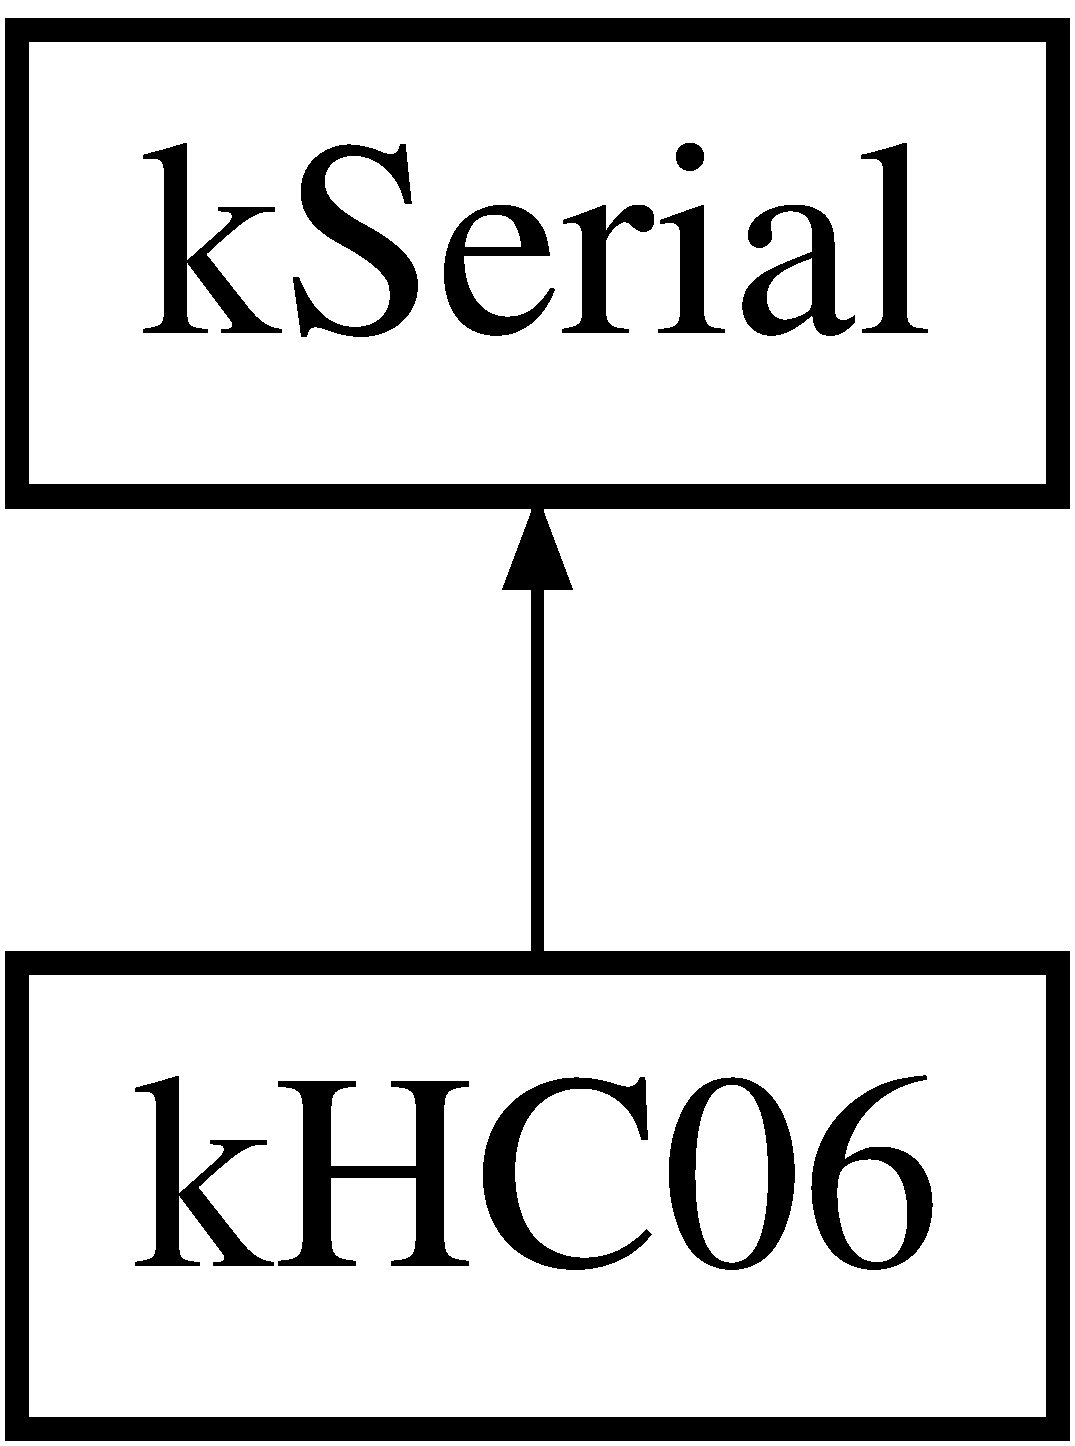
\includegraphics[height=2.000000cm]{classkHC06}
\end{center}
\end{figure}
\subsection*{Public Member Functions}
\begin{DoxyCompactItemize}
\item 
void {\bfseries set\+Name} (char $\ast$new\+\_\+name)\hypertarget{classkHC06_a20f05bfb561fd344bc9230cecba6d697}{}\label{classkHC06_a20f05bfb561fd344bc9230cecba6d697}

\item 
void {\bfseries set\+Pin} (char $\ast$new\+\_\+pin)\hypertarget{classkHC06_ae9d47c685c1130ef68c79573880183b2}{}\label{classkHC06_ae9d47c685c1130ef68c79573880183b2}

\end{DoxyCompactItemize}
\subsection*{Additional Inherited Members}


The documentation for this class was generated from the following files\+:\begin{DoxyCompactItemize}
\item 
k\+H\+C06.\+h\item 
k\+H\+C06.\+cpp\end{DoxyCompactItemize}

\hypertarget{structkI2C1}{}\section{k\+I2\+C1 Struct Reference}
\label{structkI2C1}\index{k\+I2\+C1@{k\+I2\+C1}}
\subsection*{Public Attributes}
\begin{DoxyCompactItemize}
\item 
\hyperlink{structkI2C1__SCL__Pin}{k\+I2\+C1\+\_\+\+S\+C\+L\+\_\+\+Pin} {\bfseries S\+CL}\hypertarget{structkI2C1_a894fe85cdf7fe9e0e19e5cd3290d14d8}{}\label{structkI2C1_a894fe85cdf7fe9e0e19e5cd3290d14d8}

\item 
\hyperlink{structkI2C1__SDA__Pin}{k\+I2\+C1\+\_\+\+S\+D\+A\+\_\+\+Pin} {\bfseries S\+DA}\hypertarget{structkI2C1_a8bd66305d8f3348af513e8d50140e4d9}{}\label{structkI2C1_a8bd66305d8f3348af513e8d50140e4d9}

\end{DoxyCompactItemize}


The documentation for this struct was generated from the following file\+:\begin{DoxyCompactItemize}
\item 
k\+I2\+C\+Device.\+h\end{DoxyCompactItemize}

\hypertarget{structkI2C1__SCL__Pin}{}\section{k\+I2\+C1\+\_\+\+S\+C\+L\+\_\+\+Pin Struct Reference}
\label{structkI2C1__SCL__Pin}\index{k\+I2\+C1\+\_\+\+S\+C\+L\+\_\+\+Pin@{k\+I2\+C1\+\_\+\+S\+C\+L\+\_\+\+Pin}}
\subsection*{Public Attributes}
\begin{DoxyCompactItemize}
\item 
\hyperlink{structkI2C1Pin}{k\+I2\+C1\+Pin} {\bfseries P\+O\+R\+T\+B6}\hypertarget{structkI2C1__SCL__Pin_a96c689a70a9927126b5f618ee54c35c0}{}\label{structkI2C1__SCL__Pin_a96c689a70a9927126b5f618ee54c35c0}

\item 
\hyperlink{structkI2C1Pin}{k\+I2\+C1\+Pin} {\bfseries P\+O\+R\+T\+B8}\hypertarget{structkI2C1__SCL__Pin_a35776252a186ae83a64ef260eca65a4a}{}\label{structkI2C1__SCL__Pin_a35776252a186ae83a64ef260eca65a4a}

\end{DoxyCompactItemize}


The documentation for this struct was generated from the following file\+:\begin{DoxyCompactItemize}
\item 
k\+I2\+C\+Device.\+h\end{DoxyCompactItemize}

\hypertarget{structkI2C1__SDA__Pin}{}\section{k\+I2\+C1\+\_\+\+S\+D\+A\+\_\+\+Pin Struct Reference}
\label{structkI2C1__SDA__Pin}\index{k\+I2\+C1\+\_\+\+S\+D\+A\+\_\+\+Pin@{k\+I2\+C1\+\_\+\+S\+D\+A\+\_\+\+Pin}}
\subsection*{Public Attributes}
\begin{DoxyCompactItemize}
\item 
\hyperlink{structkI2C1Pin}{k\+I2\+C1\+Pin} {\bfseries P\+O\+R\+T\+B7}\hypertarget{structkI2C1__SDA__Pin_aaea93ccfcb4fb47d21ccba0c77f8735b}{}\label{structkI2C1__SDA__Pin_aaea93ccfcb4fb47d21ccba0c77f8735b}

\item 
\hyperlink{structkI2C1Pin}{k\+I2\+C1\+Pin} {\bfseries P\+O\+R\+T\+B9}\hypertarget{structkI2C1__SDA__Pin_aecd86ce8a820396a6c0ab38be46eb1f3}{}\label{structkI2C1__SDA__Pin_aecd86ce8a820396a6c0ab38be46eb1f3}

\end{DoxyCompactItemize}


The documentation for this struct was generated from the following file\+:\begin{DoxyCompactItemize}
\item 
k\+I2\+C\+Device.\+h\end{DoxyCompactItemize}

\hypertarget{structkI2C1Pin}{}\section{k\+I2\+C1\+Pin Struct Reference}
\label{structkI2C1Pin}\index{k\+I2\+C1\+Pin@{k\+I2\+C1\+Pin}}
\subsection*{Public Attributes}
\begin{DoxyCompactItemize}
\item 
unsigned char {\bfseries k\+I2\+C1pin}\hypertarget{structkI2C1Pin_abae5bc275d80ea00f33ec2af9c79d255}{}\label{structkI2C1Pin_abae5bc275d80ea00f33ec2af9c79d255}

\end{DoxyCompactItemize}


The documentation for this struct was generated from the following file\+:\begin{DoxyCompactItemize}
\item 
k\+I2\+C\+Device.\+h\end{DoxyCompactItemize}

\hypertarget{structkI2C2}{}\section{k\+I2\+C2 Struct Reference}
\label{structkI2C2}\index{k\+I2\+C2@{k\+I2\+C2}}
\subsection*{Public Attributes}
\begin{DoxyCompactItemize}
\item 
\hyperlink{structkI2C2__SCL__Pin}{k\+I2\+C2\+\_\+\+S\+C\+L\+\_\+\+Pin} {\bfseries S\+CL}\hypertarget{structkI2C2_af8670468793d611e1598e4b3978fc8ce}{}\label{structkI2C2_af8670468793d611e1598e4b3978fc8ce}

\item 
\hyperlink{structkI2C2__SDA__Pin}{k\+I2\+C2\+\_\+\+S\+D\+A\+\_\+\+Pin} {\bfseries S\+DA}\hypertarget{structkI2C2_a6fe2ef204657e0d784c8b4b4fe472ce6}{}\label{structkI2C2_a6fe2ef204657e0d784c8b4b4fe472ce6}

\end{DoxyCompactItemize}


The documentation for this struct was generated from the following file\+:\begin{DoxyCompactItemize}
\item 
k\+I2\+C\+Device.\+h\end{DoxyCompactItemize}

\hypertarget{structkI2C2__SCL__Pin}{}\section{k\+I2\+C2\+\_\+\+S\+C\+L\+\_\+\+Pin Struct Reference}
\label{structkI2C2__SCL__Pin}\index{k\+I2\+C2\+\_\+\+S\+C\+L\+\_\+\+Pin@{k\+I2\+C2\+\_\+\+S\+C\+L\+\_\+\+Pin}}
\subsection*{Public Attributes}
\begin{DoxyCompactItemize}
\item 
\hyperlink{structkI2C2Pin}{k\+I2\+C2\+Pin} {\bfseries P\+O\+R\+T\+B10}\hypertarget{structkI2C2__SCL__Pin_afa10933edaab723e127a2d115a920d0b}{}\label{structkI2C2__SCL__Pin_afa10933edaab723e127a2d115a920d0b}

\item 
\hyperlink{structkI2C2Pin}{k\+I2\+C2\+Pin} {\bfseries P\+O\+R\+T\+F1}\hypertarget{structkI2C2__SCL__Pin_ad6d5dae9cc4cbb930b73bd6175ae8e58}{}\label{structkI2C2__SCL__Pin_ad6d5dae9cc4cbb930b73bd6175ae8e58}

\item 
\hyperlink{structkI2C2Pin}{k\+I2\+C2\+Pin} {\bfseries P\+O\+R\+T\+H4}\hypertarget{structkI2C2__SCL__Pin_ab260b3448820d5eabb951a78f0fe10db}{}\label{structkI2C2__SCL__Pin_ab260b3448820d5eabb951a78f0fe10db}

\end{DoxyCompactItemize}


The documentation for this struct was generated from the following file\+:\begin{DoxyCompactItemize}
\item 
k\+I2\+C\+Device.\+h\end{DoxyCompactItemize}

\hypertarget{structkI2C2__SDA__Pin}{}\section{k\+I2\+C2\+\_\+\+S\+D\+A\+\_\+\+Pin Struct Reference}
\label{structkI2C2__SDA__Pin}\index{k\+I2\+C2\+\_\+\+S\+D\+A\+\_\+\+Pin@{k\+I2\+C2\+\_\+\+S\+D\+A\+\_\+\+Pin}}
\subsection*{Public Attributes}
\begin{DoxyCompactItemize}
\item 
\hyperlink{structkI2C2Pin}{k\+I2\+C2\+Pin} {\bfseries P\+O\+R\+T\+B11}\hypertarget{structkI2C2__SDA__Pin_a5fff55f4ae1d93b24a3a3cbde8cab051}{}\label{structkI2C2__SDA__Pin_a5fff55f4ae1d93b24a3a3cbde8cab051}

\item 
\hyperlink{structkI2C2Pin}{k\+I2\+C2\+Pin} {\bfseries P\+O\+R\+T\+F0}\hypertarget{structkI2C2__SDA__Pin_aa119d3b0d6c6fefd1e3fb5a3402408d0}{}\label{structkI2C2__SDA__Pin_aa119d3b0d6c6fefd1e3fb5a3402408d0}

\item 
\hyperlink{structkI2C2Pin}{k\+I2\+C2\+Pin} {\bfseries P\+O\+R\+T\+H5}\hypertarget{structkI2C2__SDA__Pin_a82f154f9dfe4bf0b9d5f089e51ae59de}{}\label{structkI2C2__SDA__Pin_a82f154f9dfe4bf0b9d5f089e51ae59de}

\end{DoxyCompactItemize}


The documentation for this struct was generated from the following file\+:\begin{DoxyCompactItemize}
\item 
k\+I2\+C\+Device.\+h\end{DoxyCompactItemize}

\hypertarget{structkI2C2Pin}{}\section{k\+I2\+C2\+Pin Struct Reference}
\label{structkI2C2Pin}\index{k\+I2\+C2\+Pin@{k\+I2\+C2\+Pin}}
\subsection*{Public Attributes}
\begin{DoxyCompactItemize}
\item 
unsigned char {\bfseries k\+I2\+C1pin}\hypertarget{structkI2C2Pin_a9a9957ef7a6a1f2de830f23f9cc9f2f5}{}\label{structkI2C2Pin_a9a9957ef7a6a1f2de830f23f9cc9f2f5}

\end{DoxyCompactItemize}


The documentation for this struct was generated from the following file\+:\begin{DoxyCompactItemize}
\item 
k\+I2\+C\+Device.\+h\end{DoxyCompactItemize}

\hypertarget{structkI2C3}{}\section{k\+I2\+C3 Struct Reference}
\label{structkI2C3}\index{k\+I2\+C3@{k\+I2\+C3}}
\subsection*{Public Attributes}
\begin{DoxyCompactItemize}
\item 
\hyperlink{structkI2C3__SCL__Pin}{k\+I2\+C3\+\_\+\+S\+C\+L\+\_\+\+Pin} {\bfseries S\+CL}\hypertarget{structkI2C3_a4d3320e6a2554446714e9c24dc769663}{}\label{structkI2C3_a4d3320e6a2554446714e9c24dc769663}

\item 
\hyperlink{structkI2C3__SDA__Pin}{k\+I2\+C3\+\_\+\+S\+D\+A\+\_\+\+Pin} {\bfseries S\+DA}\hypertarget{structkI2C3_ac687d9e2fa7c15455bf2a489a440eafb}{}\label{structkI2C3_ac687d9e2fa7c15455bf2a489a440eafb}

\end{DoxyCompactItemize}


The documentation for this struct was generated from the following file\+:\begin{DoxyCompactItemize}
\item 
k\+I2\+C\+Device.\+h\end{DoxyCompactItemize}

\hypertarget{structkI2C3__SCL__Pin}{}\section{k\+I2\+C3\+\_\+\+S\+C\+L\+\_\+\+Pin Struct Reference}
\label{structkI2C3__SCL__Pin}\index{k\+I2\+C3\+\_\+\+S\+C\+L\+\_\+\+Pin@{k\+I2\+C3\+\_\+\+S\+C\+L\+\_\+\+Pin}}
\subsection*{Public Attributes}
\begin{DoxyCompactItemize}
\item 
\hyperlink{structkI2C3Pin}{k\+I2\+C3\+Pin} {\bfseries P\+O\+R\+T\+A8}\hypertarget{structkI2C3__SCL__Pin_a14949c3931d045ef7307658ca6be2fb8}{}\label{structkI2C3__SCL__Pin_a14949c3931d045ef7307658ca6be2fb8}

\item 
\hyperlink{structkI2C3Pin}{k\+I2\+C3\+Pin} {\bfseries P\+O\+R\+T\+H7}\hypertarget{structkI2C3__SCL__Pin_a8d579234046c306a14b93a4f1878c0e9}{}\label{structkI2C3__SCL__Pin_a8d579234046c306a14b93a4f1878c0e9}

\end{DoxyCompactItemize}


The documentation for this struct was generated from the following file\+:\begin{DoxyCompactItemize}
\item 
k\+I2\+C\+Device.\+h\end{DoxyCompactItemize}

\hypertarget{structkI2C3__SDA__Pin}{}\section{k\+I2\+C3\+\_\+\+S\+D\+A\+\_\+\+Pin Struct Reference}
\label{structkI2C3__SDA__Pin}\index{k\+I2\+C3\+\_\+\+S\+D\+A\+\_\+\+Pin@{k\+I2\+C3\+\_\+\+S\+D\+A\+\_\+\+Pin}}
\subsection*{Public Attributes}
\begin{DoxyCompactItemize}
\item 
\hyperlink{structkI2C3Pin}{k\+I2\+C3\+Pin} {\bfseries P\+O\+R\+T\+C9}\hypertarget{structkI2C3__SDA__Pin_a2604936300310d9b0b7c5058bd375e11}{}\label{structkI2C3__SDA__Pin_a2604936300310d9b0b7c5058bd375e11}

\item 
\hyperlink{structkI2C3Pin}{k\+I2\+C3\+Pin} {\bfseries P\+O\+R\+T\+H8}\hypertarget{structkI2C3__SDA__Pin_ab7d36d0237fbc10b02631067f9f8d382}{}\label{structkI2C3__SDA__Pin_ab7d36d0237fbc10b02631067f9f8d382}

\end{DoxyCompactItemize}


The documentation for this struct was generated from the following file\+:\begin{DoxyCompactItemize}
\item 
k\+I2\+C\+Device.\+h\end{DoxyCompactItemize}

\hypertarget{structkI2C3Pin}{}\section{k\+I2\+C3\+Pin Struct Reference}
\label{structkI2C3Pin}\index{k\+I2\+C3\+Pin@{k\+I2\+C3\+Pin}}
\subsection*{Public Attributes}
\begin{DoxyCompactItemize}
\item 
unsigned char {\bfseries k\+I2\+C3pin}\hypertarget{structkI2C3Pin_a3c51fb13a36f122f537386a1795357ab}{}\label{structkI2C3Pin_a3c51fb13a36f122f537386a1795357ab}

\end{DoxyCompactItemize}


The documentation for this struct was generated from the following file\+:\begin{DoxyCompactItemize}
\item 
k\+I2\+C\+Device.\+h\end{DoxyCompactItemize}

\hypertarget{classkI2CDevice}{}\section{k\+I2\+C\+Device Class Reference}
\label{classkI2CDevice}\index{k\+I2\+C\+Device@{k\+I2\+C\+Device}}
\subsection*{Public Member Functions}
\begin{DoxyCompactItemize}
\item 
{\bfseries k\+I2\+C\+Device} (const \hyperlink{structkI2C1Pin}{k\+I2\+C1\+Pin} \&S\+CL, const \hyperlink{structkI2C1Pin}{k\+I2\+C1\+Pin} \&S\+DA, unsigned int clock\+Speed)\hypertarget{classkI2CDevice_ad4ea485f71060c28713e55a23fd05b86}{}\label{classkI2CDevice_ad4ea485f71060c28713e55a23fd05b86}

\item 
{\bfseries k\+I2\+C\+Device} (const \hyperlink{structkI2C2Pin}{k\+I2\+C2\+Pin} \&S\+CL, const \hyperlink{structkI2C2Pin}{k\+I2\+C2\+Pin} \&S\+DA, unsigned int clock\+Speed)\hypertarget{classkI2CDevice_adbb52b2b61c0358a015af1fa71de83ea}{}\label{classkI2CDevice_adbb52b2b61c0358a015af1fa71de83ea}

\item 
{\bfseries k\+I2\+C\+Device} (const \hyperlink{structkI2C3Pin}{k\+I2\+C3\+Pin} \&S\+CL, const \hyperlink{structkI2C3Pin}{k\+I2\+C3\+Pin} \&S\+DA, unsigned int clock\+Speed)\hypertarget{classkI2CDevice_a1ff149208c797fe3619b233930340ac7}{}\label{classkI2CDevice_a1ff149208c797fe3619b233930340ac7}

\item 
void {\bfseries write} (uint8\+\_\+t Starting\+Register\+Address, uint8\+\_\+t $\ast$transmit\+\_\+buffer, uint8\+\_\+t Bytes\+To\+Write)\hypertarget{classkI2CDevice_a777e881385da3b286d99fd74c20a90dc}{}\label{classkI2CDevice_a777e881385da3b286d99fd74c20a90dc}

\item 
void {\bfseries write} (uint8\+\_\+t Register\+Address, uint8\+\_\+t value)\hypertarget{classkI2CDevice_a5bbe4810f14dc08693240b2a82e83c51}{}\label{classkI2CDevice_a5bbe4810f14dc08693240b2a82e83c51}

\item 
void {\bfseries read} (uint8\+\_\+t Starting\+Register\+Address, uint8\+\_\+t $\ast$recieve\+\_\+buffer, uint8\+\_\+t Bytes\+To\+Read)\hypertarget{classkI2CDevice_aee7738a6e13e451f59ff5ec5e98ced21}{}\label{classkI2CDevice_aee7738a6e13e451f59ff5ec5e98ced21}

\item 
unsigned char {\bfseries read} (uint8\+\_\+t Register\+Address)\hypertarget{classkI2CDevice_af9185267e48384e0d717d5792a80232b}{}\label{classkI2CDevice_af9185267e48384e0d717d5792a80232b}

\end{DoxyCompactItemize}
\subsection*{Public Attributes}
\begin{DoxyCompactItemize}
\item 
\hyperlink{classkI2CDeviceHardware}{k\+I2\+C\+Device\+Hardware} {\bfseries hardware}\hypertarget{classkI2CDevice_a2572571c46a1ddb9dbee0882f98cf5f4}{}\label{classkI2CDevice_a2572571c46a1ddb9dbee0882f98cf5f4}

\item 
unsigned char {\bfseries I2\+C\+\_\+\+Address}\hypertarget{classkI2CDevice_a226a4250afdfc9c9607dc2efc72d97e5}{}\label{classkI2CDevice_a226a4250afdfc9c9607dc2efc72d97e5}

\end{DoxyCompactItemize}
\subsection*{Static Public Attributes}
\begin{DoxyCompactItemize}
\item 
static const \hyperlink{structkI2C1}{k\+I2\+C1} $\ast$ {\bfseries I2\+C\+\_\+1} = (\hyperlink{structkI2C1}{k\+I2\+C1} $\ast$)S\+R\+A\+M1\+\_\+\+B\+A\+SE\hypertarget{classkI2CDevice_abf6aae166d28e3c81f503b6c96fdc6d5}{}\label{classkI2CDevice_abf6aae166d28e3c81f503b6c96fdc6d5}

\item 
static const \hyperlink{structkI2C2}{k\+I2\+C2} $\ast$ {\bfseries I2\+C\+\_\+2} = (\hyperlink{structkI2C2}{k\+I2\+C2} $\ast$)S\+R\+A\+M1\+\_\+\+B\+A\+SE\hypertarget{classkI2CDevice_a8042ffc9d65f22469819ecfa78abe84d}{}\label{classkI2CDevice_a8042ffc9d65f22469819ecfa78abe84d}

\item 
static const \hyperlink{structkI2C3}{k\+I2\+C3} $\ast$ {\bfseries I2\+C\+\_\+3} = (\hyperlink{structkI2C3}{k\+I2\+C3} $\ast$)S\+R\+A\+M1\+\_\+\+B\+A\+SE\hypertarget{classkI2CDevice_a0f0c6ced2cc7f36b77171c2dd0130784}{}\label{classkI2CDevice_a0f0c6ced2cc7f36b77171c2dd0130784}

\end{DoxyCompactItemize}


The documentation for this class was generated from the following files\+:\begin{DoxyCompactItemize}
\item 
k\+I2\+C\+Device.\+h\item 
k\+I2\+C\+Device.\+cpp\end{DoxyCompactItemize}

\hypertarget{classkI2CDeviceHardware}{}\section{k\+I2\+C\+Device\+Hardware Class Reference}
\label{classkI2CDeviceHardware}\index{k\+I2\+C\+Device\+Hardware@{k\+I2\+C\+Device\+Hardware}}
\subsection*{Public Member Functions}
\begin{DoxyCompactItemize}
\item 
void {\bfseries operator=} (const \hyperlink{structkI2C1Pin}{k\+I2\+C1\+Pin} \&i2c\+Hard)\hypertarget{classkI2CDeviceHardware_a679af91213606c5b4578ff339de3ee6f}{}\label{classkI2CDeviceHardware_a679af91213606c5b4578ff339de3ee6f}

\item 
void {\bfseries operator=} (const \hyperlink{structkI2C2Pin}{k\+I2\+C2\+Pin} \&i2c\+Hard)\hypertarget{classkI2CDeviceHardware_a080dcae96ac9be37809fcd68d32cc78e}{}\label{classkI2CDeviceHardware_a080dcae96ac9be37809fcd68d32cc78e}

\item 
void {\bfseries operator=} (const \hyperlink{structkI2C3Pin}{k\+I2\+C3\+Pin} \&i2c\+Hard)\hypertarget{classkI2CDeviceHardware_a391bdcaf62518e322c207ae755255a01}{}\label{classkI2CDeviceHardware_a391bdcaf62518e322c207ae755255a01}

\item 
void {\bfseries setup\+S\+C\+L\+Pin} (void)\hypertarget{classkI2CDeviceHardware_acd2d326416a95b0f1bfacef5a060bce8}{}\label{classkI2CDeviceHardware_acd2d326416a95b0f1bfacef5a060bce8}

\item 
void {\bfseries setup\+S\+D\+A\+Pin} (void)\hypertarget{classkI2CDeviceHardware_a9659890e2121651836f69c3923ac7ea4}{}\label{classkI2CDeviceHardware_a9659890e2121651836f69c3923ac7ea4}

\item 
void {\bfseries clock\+Speed} (unsigned int value)\hypertarget{classkI2CDeviceHardware_ad34d314130ee0d6b9181963913f5f367}{}\label{classkI2CDeviceHardware_ad34d314130ee0d6b9181963913f5f367}

\end{DoxyCompactItemize}
\subsection*{Public Attributes}
\begin{DoxyCompactItemize}
\item 
I2\+C\+\_\+\+Type\+Def $\ast$ {\bfseries i2c}\hypertarget{classkI2CDeviceHardware_ace7b414f13cbd3e93e904c661cc02e35}{}\label{classkI2CDeviceHardware_ace7b414f13cbd3e93e904c661cc02e35}

\item 
G\+P\+I\+O\+\_\+\+Type\+Def $\ast$ {\bfseries sda\+G\+P\+IO}\hypertarget{classkI2CDeviceHardware_af0228a16a473dfdd0f33ae6f60eb6cfc}{}\label{classkI2CDeviceHardware_af0228a16a473dfdd0f33ae6f60eb6cfc}

\item 
G\+P\+I\+O\+\_\+\+Type\+Def $\ast$ {\bfseries scl\+G\+P\+IO}\hypertarget{classkI2CDeviceHardware_ab4433caa4d8c1b7c460fd0c356ce87c0}{}\label{classkI2CDeviceHardware_ab4433caa4d8c1b7c460fd0c356ce87c0}

\item 
unsigned char {\bfseries sda\+Pin}\hypertarget{classkI2CDeviceHardware_ac244794bc64bf54acf12bc43242b7a13}{}\label{classkI2CDeviceHardware_ac244794bc64bf54acf12bc43242b7a13}

\item 
unsigned char {\bfseries scl\+Pin}\hypertarget{classkI2CDeviceHardware_a33ccd2758d40a159e023e6f338726fa8}{}\label{classkI2CDeviceHardware_a33ccd2758d40a159e023e6f338726fa8}

\end{DoxyCompactItemize}


The documentation for this class was generated from the following files\+:\begin{DoxyCompactItemize}
\item 
k\+I2\+C\+Device.\+h\item 
k\+I2\+C\+Device.\+cpp\end{DoxyCompactItemize}

\hypertarget{classkMatrix}{}\section{k\+Matrix Class Reference}
\label{classkMatrix}\index{k\+Matrix@{k\+Matrix}}
\subsection*{Public Member Functions}
\begin{DoxyCompactItemize}
\item 
{\bfseries k\+Matrix} (unsigned char square\+\_\+dimension)\hypertarget{classkMatrix_a5868ea1a392cab2599fe6800b5581d28}{}\label{classkMatrix_a5868ea1a392cab2599fe6800b5581d28}

\item 
{\bfseries k\+Matrix} (unsigned char rows, unsigned char cols)\hypertarget{classkMatrix_a28984eea87a03bff5b518713990f0eb9}{}\label{classkMatrix_a28984eea87a03bff5b518713990f0eb9}

\item 
unsigned char {\bfseries rows} (void)\hypertarget{classkMatrix_a364788171666de4935792ca12cad3b49}{}\label{classkMatrix_a364788171666de4935792ca12cad3b49}

\item 
unsigned char {\bfseries cols} (void)\hypertarget{classkMatrix_ae4e1b7b151a356b932e1c2b663e3107a}{}\label{classkMatrix_ae4e1b7b151a356b932e1c2b663e3107a}

\item 
unsigned char {\bfseries size} (void)\hypertarget{classkMatrix_a572b1a6fcb9d99b2ba449af7d76ab1ae}{}\label{classkMatrix_a572b1a6fcb9d99b2ba449af7d76ab1ae}

\item 
float \& {\bfseries operator()} (unsigned char row, unsigned char column)\hypertarget{classkMatrix_a8cda547bb01fb1730c5bac921c777c4e}{}\label{classkMatrix_a8cda547bb01fb1730c5bac921c777c4e}

\item 
void {\bfseries operator=} (const \hyperlink{classkMatrix}{k\+Matrix} \&other)\hypertarget{classkMatrix_a6111aac12009c07addb52950cd6f282a}{}\label{classkMatrix_a6111aac12009c07addb52950cd6f282a}

\item 
\hyperlink{classkMatrix}{k\+Matrix} \& {\bfseries operator=} (float num)\hypertarget{classkMatrix_ad2a5d42acda3da64177be9f897979baa}{}\label{classkMatrix_ad2a5d42acda3da64177be9f897979baa}

\item 
void {\bfseries operator+=} (const \hyperlink{classkMatrix}{k\+Matrix} \&other)\hypertarget{classkMatrix_a131671a495a5412ceaff23e092bfec9b}{}\label{classkMatrix_a131671a495a5412ceaff23e092bfec9b}

\item 
void {\bfseries operator-\/=} (const \hyperlink{classkMatrix}{k\+Matrix} \&other)\hypertarget{classkMatrix_ab40d193c22733471d33bceda42bf1213}{}\label{classkMatrix_ab40d193c22733471d33bceda42bf1213}

\item 
void {\bfseries operator$\ast$=} (\hyperlink{classkMatrix}{k\+Matrix} \&other)\hypertarget{classkMatrix_ac0dccc61cfbabe1da72726559b33cbdf}{}\label{classkMatrix_ac0dccc61cfbabe1da72726559b33cbdf}

\item 
\hyperlink{classkMatrix}{k\+Matrix} \& {\bfseries operator,} (float num)\hypertarget{classkMatrix_a89251b25202e1ae2b7e2fd2b9b4840c4}{}\label{classkMatrix_a89251b25202e1ae2b7e2fd2b9b4840c4}

\item 
float {\bfseries det} (void)\hypertarget{classkMatrix_af2e75801e4461b4d7807741559c73bad}{}\label{classkMatrix_af2e75801e4461b4d7807741559c73bad}

\end{DoxyCompactItemize}
\subsection*{Friends}
\begin{DoxyCompactItemize}
\item 
\hyperlink{classkMatrix}{k\+Matrix} {\bfseries operator+} (const \hyperlink{classkMatrix}{k\+Matrix} \&m1, const \hyperlink{classkMatrix}{k\+Matrix} \&m2)\hypertarget{classkMatrix_a9b9d61523004337a496065dd5cea0d54}{}\label{classkMatrix_a9b9d61523004337a496065dd5cea0d54}

\item 
\hyperlink{classkMatrix}{k\+Matrix} {\bfseries operator-\/} (const \hyperlink{classkMatrix}{k\+Matrix} \&m1, const \hyperlink{classkMatrix}{k\+Matrix} \&m2)\hypertarget{classkMatrix_a267db7ca0cd79f373da986853d070d88}{}\label{classkMatrix_a267db7ca0cd79f373da986853d070d88}

\item 
\hyperlink{classkMatrix}{k\+Matrix} {\bfseries operator$\ast$} (\hyperlink{classkMatrix}{k\+Matrix} \&m1, \hyperlink{classkMatrix}{k\+Matrix} \&m2)\hypertarget{classkMatrix_a65c60053d2f8f7331833722980162ba4}{}\label{classkMatrix_a65c60053d2f8f7331833722980162ba4}

\end{DoxyCompactItemize}


The documentation for this class was generated from the following files\+:\begin{DoxyCompactItemize}
\item 
k\+Matrix.\+h\item 
k\+Matrix.\+cpp\end{DoxyCompactItemize}

\hypertarget{classkPin}{}\section{k\+Pin Class Reference}
\label{classkPin}\index{k\+Pin@{k\+Pin}}


\hyperlink{classkPin}{k\+Pin} class is used as abstract layer to handle input/output pin functionality  




{\ttfamily \#include $<$k\+Port.\+h$>$}

\subsection*{Public Types}
\begin{DoxyCompactItemize}
\item 
enum \hyperlink{classkPin_a311ea70432d9c48754eacc8d8ce8a949}{k\+Pin\+Mode} \{ \hyperlink{classkPin_a311ea70432d9c48754eacc8d8ce8a949a554230cb796f1567722de2f735e49aeb}{in}, 
\hyperlink{classkPin_a311ea70432d9c48754eacc8d8ce8a949acafa1712464c40b469cd18209d298967}{out}, 
\hyperlink{classkPin_a311ea70432d9c48754eacc8d8ce8a949a90e36f24bfc26ff0c10878e9339c0eef}{alternate}, 
\hyperlink{classkPin_a311ea70432d9c48754eacc8d8ce8a949a38b78e28a019a75bc66237f45d5752a0}{analog}
 \}\begin{DoxyCompactList}\small\item\em Contains available pin modes. \end{DoxyCompactList}
\item 
enum \hyperlink{classkPin_a5aa9350fb0a7617a568344d8a074837f}{k\+Pin\+Out\+Type} \{ \hyperlink{classkPin_a5aa9350fb0a7617a568344d8a074837fa91ae703d8d54aa82385684e9fcd89190}{Push\+Pull}, 
\hyperlink{classkPin_a5aa9350fb0a7617a568344d8a074837fa0f1c262ab8465ee84ca83377044c6c07}{Open\+Drain}
 \}\begin{DoxyCompactList}\small\item\em Definition of type containing output mode types. \end{DoxyCompactList}
\item 
enum \hyperlink{classkPin_a4d00e25b986e7851957a68deb1c91b18}{k\+Pull\+Resistor} \{ \hyperlink{classkPin_a4d00e25b986e7851957a68deb1c91b18afed0e5fed525988ffab024b212f778de}{No\+Pull}, 
\hyperlink{classkPin_a4d00e25b986e7851957a68deb1c91b18a149a20dc06140c63aa9939f0f974823d}{Pull\+Up}, 
\hyperlink{classkPin_a4d00e25b986e7851957a68deb1c91b18a494be2d7584a71eb80aad5008bb52e9a}{Pull\+Down}
 \}\begin{DoxyCompactList}\small\item\em Definition of type containing pull resistors settings. \end{DoxyCompactList}
\item 
enum \hyperlink{classkPin_a93c5cec6b9b90fda782cfa847eacdb8b}{k\+Pin\+Speed} \{ \hyperlink{classkPin_a93c5cec6b9b90fda782cfa847eacdb8babf1cc1c1725ace9389d0ec589abfbc95}{Low\+Speed}, 
\hyperlink{classkPin_a93c5cec6b9b90fda782cfa847eacdb8bab65b9156fa586ff9e9cdca7d8cdcf3d0}{Medium\+Speed}, 
\hyperlink{classkPin_a93c5cec6b9b90fda782cfa847eacdb8ba42a2d420a8ca9da17870c1a0ebc89d89}{High\+Speed}, 
\hyperlink{classkPin_a93c5cec6b9b90fda782cfa847eacdb8ba637da5063c11dbfb83b98ea6a2d84588}{Very\+High\+Speed}
 \}\begin{DoxyCompactList}\small\item\em Definition of type containing maximum state toggling frequencies of pin. \end{DoxyCompactList}
\end{DoxyCompactItemize}
\subsection*{Public Member Functions}
\begin{DoxyCompactItemize}
\item 
\hyperlink{classkPin_a6298d5af7b3abb27ba12e91a926b124b}{k\+Pin} (void)\hypertarget{classkPin_a6298d5af7b3abb27ba12e91a926b124b}{}\label{classkPin_a6298d5af7b3abb27ba12e91a926b124b}

\begin{DoxyCompactList}\small\item\em Default constructor. \end{DoxyCompactList}\item 
\hyperlink{classkPin_ab566517aa9b1985a0c1093e193730c9d}{k\+Pin} (G\+P\+I\+O\+\_\+\+Type\+Def $\ast$G\+P\+IO, unsigned char P\+IN)
\begin{DoxyCompactList}\small\item\em Constructor with hardware attachment. \end{DoxyCompactList}\item 
\hyperlink{classkPin_a6c7f13462a99ba72e558cfcb389476f6}{k\+Pin} (const \hyperlink{classkPin}{k\+Pin} \&\hyperlink{classkPin_a0da283781fc832c77419bc71ff356cc1}{pin})
\begin{DoxyCompactList}\small\item\em Copy constructor. \end{DoxyCompactList}\item 
unsigned char \hyperlink{classkPin_a2ef21ca53fb82456997485b14bac45b0}{get} (void)
\begin{DoxyCompactList}\small\item\em Get actual state on pin. \end{DoxyCompactList}\item 
void \hyperlink{classkPin_a5f02fd984651e5a9e92bd3218d8e4bd0}{set} (void)\hypertarget{classkPin_a5f02fd984651e5a9e92bd3218d8e4bd0}{}\label{classkPin_a5f02fd984651e5a9e92bd3218d8e4bd0}

\begin{DoxyCompactList}\small\item\em set pin (writes 1), this function has an effect only in output mode \end{DoxyCompactList}\item 
void \hyperlink{classkPin_af6c53f90a2f1984bbfb045e75c14f933}{reset} (void)\hypertarget{classkPin_af6c53f90a2f1984bbfb045e75c14f933}{}\label{classkPin_af6c53f90a2f1984bbfb045e75c14f933}

\begin{DoxyCompactList}\small\item\em reset pin (writes 0), this function has an effect only in output mode \end{DoxyCompactList}\item 
void \hyperlink{classkPin_af4c6220ae2ed038236d729f867940938}{toggle} (void)\hypertarget{classkPin_af4c6220ae2ed038236d729f867940938}{}\label{classkPin_af4c6220ae2ed038236d729f867940938}

\begin{DoxyCompactList}\small\item\em toggle state on pin (when 1 set to 0; when 0 set to 1), this function has an effect only in output mode \end{DoxyCompactList}\item 
void {\bfseries operator=} (unsigned char state)\hypertarget{classkPin_a3c4330824805701cbcb52431b187f643}{}\label{classkPin_a3c4330824805701cbcb52431b187f643}

\item 
const \hyperlink{classkPin}{k\+Pin} \& {\bfseries operator=} (\hyperlink{classkPin_a311ea70432d9c48754eacc8d8ce8a949}{k\+Pin\+Mode} mode)\hypertarget{classkPin_aaaad528a43da36662f4361d13419b0c0}{}\label{classkPin_aaaad528a43da36662f4361d13419b0c0}

\item 
const \hyperlink{classkPin}{k\+Pin} \& {\bfseries operator=} (\hyperlink{classkPin_a5aa9350fb0a7617a568344d8a074837f}{k\+Pin\+Out\+Type} out\+Type)\hypertarget{classkPin_a32d7ae0a031264b9f47a8c691ae16a1e}{}\label{classkPin_a32d7ae0a031264b9f47a8c691ae16a1e}

\item 
const \hyperlink{classkPin}{k\+Pin} \& {\bfseries operator=} (\hyperlink{classkPin_a4d00e25b986e7851957a68deb1c91b18}{k\+Pull\+Resistor} pull\+Resistor)\hypertarget{classkPin_af5fd9228e54385316b644f190c6f5dfc}{}\label{classkPin_af5fd9228e54385316b644f190c6f5dfc}

\item 
const \hyperlink{classkPin}{k\+Pin} \& {\bfseries operator=} (\hyperlink{classkPin_a93c5cec6b9b90fda782cfa847eacdb8b}{k\+Pin\+Speed} speed)\hypertarget{classkPin_a91238da7b4019164f8205f8a3219628d}{}\label{classkPin_a91238da7b4019164f8205f8a3219628d}

\item 
void {\bfseries operator=} (\hyperlink{classkPin}{k\+Pin} \&\hyperlink{classkPin_a0da283781fc832c77419bc71ff356cc1}{pin})\hypertarget{classkPin_aef0f51fbe34f5a0c05cb98669e80dc4f}{}\label{classkPin_aef0f51fbe34f5a0c05cb98669e80dc4f}

\item 
\hyperlink{classkPin_ad68a3e0f49384a776ddd955a7258e95f}{operator unsigned char} ()\hypertarget{classkPin_ad68a3e0f49384a776ddd955a7258e95f}{}\label{classkPin_ad68a3e0f49384a776ddd955a7258e95f}

\begin{DoxyCompactList}\small\item\em specifies conversion from \hyperlink{classkPin}{k\+Pin} to unsigned char. This function is equal to \hyperlink{classkPin_a2ef21ca53fb82456997485b14bac45b0}{get()} function \end{DoxyCompactList}\end{DoxyCompactItemize}
\subsection*{Public Attributes}
\begin{DoxyCompactItemize}
\item 
G\+P\+I\+O\+\_\+\+Type\+Def $\ast$ \hyperlink{classkPin_a3aee22ce5c4e5bc8703f881efa5f3375}{gpio}
\item 
unsigned char \hyperlink{classkPin_a0da283781fc832c77419bc71ff356cc1}{pin}
\end{DoxyCompactItemize}
\subsection*{Friends}
\begin{DoxyCompactItemize}
\item 
const \hyperlink{classkPin}{k\+Pin} \& {\bfseries operator,} (const \hyperlink{classkPin}{k\+Pin} \&\hyperlink{classkPin_a0da283781fc832c77419bc71ff356cc1}{pin}, \hyperlink{classkPin_a311ea70432d9c48754eacc8d8ce8a949}{k\+Pin\+Mode} mode)\hypertarget{classkPin_ab0ba0ce3d6f1a0f08480748e102cd0ba}{}\label{classkPin_ab0ba0ce3d6f1a0f08480748e102cd0ba}

\item 
const \hyperlink{classkPin}{k\+Pin} \& {\bfseries operator,} (const \hyperlink{classkPin}{k\+Pin} \&\hyperlink{classkPin_a0da283781fc832c77419bc71ff356cc1}{pin}, \hyperlink{classkPin_a5aa9350fb0a7617a568344d8a074837f}{k\+Pin\+Out\+Type} out\+Type)\hypertarget{classkPin_a19d953ec4a8e71818ba72d18d769cda2}{}\label{classkPin_a19d953ec4a8e71818ba72d18d769cda2}

\item 
const \hyperlink{classkPin}{k\+Pin} \& {\bfseries operator,} (const \hyperlink{classkPin}{k\+Pin} \&\hyperlink{classkPin_a0da283781fc832c77419bc71ff356cc1}{pin}, \hyperlink{classkPin_a4d00e25b986e7851957a68deb1c91b18}{k\+Pull\+Resistor} pull\+Resistor)\hypertarget{classkPin_a53b5fbd0822536e24e4d01af9871b216}{}\label{classkPin_a53b5fbd0822536e24e4d01af9871b216}

\item 
const \hyperlink{classkPin}{k\+Pin} \& {\bfseries operator,} (const \hyperlink{classkPin}{k\+Pin} \&\hyperlink{classkPin_a0da283781fc832c77419bc71ff356cc1}{pin}, \hyperlink{classkPin_a93c5cec6b9b90fda782cfa847eacdb8b}{k\+Pin\+Speed} speed)\hypertarget{classkPin_a68646ef55ab985565d1119ebf4a4cf2f}{}\label{classkPin_a68646ef55ab985565d1119ebf4a4cf2f}

\end{DoxyCompactItemize}


\subsection{Detailed Description}
\hyperlink{classkPin}{k\+Pin} class is used as abstract layer to handle input/output pin functionality \begin{Desc}
\item[Examples\+: ]\par
\hyperlink{kPort_example_LED_8cpp-example}{k\+Port\+\_\+example\+\_\+\+L\+E\+D.\+cpp}.\end{Desc}


\subsection{Member Enumeration Documentation}
\index{k\+Pin@{k\+Pin}!k\+Pin\+Mode@{k\+Pin\+Mode}}
\index{k\+Pin\+Mode@{k\+Pin\+Mode}!k\+Pin@{k\+Pin}}
\subsubsection[{\texorpdfstring{k\+Pin\+Mode}{kPinMode}}]{\setlength{\rightskip}{0pt plus 5cm}enum {\bf k\+Pin\+::k\+Pin\+Mode}}\hypertarget{classkPin_a311ea70432d9c48754eacc8d8ce8a949}{}\label{classkPin_a311ea70432d9c48754eacc8d8ce8a949}


Contains available pin modes. 

\begin{Desc}
\item[Enumerator]\par
\begin{description}
\index{in@{in}!k\+Pin@{k\+Pin}}\index{k\+Pin@{k\+Pin}!in@{in}}\item[{\em 
in\hypertarget{classkPin_a311ea70432d9c48754eacc8d8ce8a949a554230cb796f1567722de2f735e49aeb}{}\label{classkPin_a311ea70432d9c48754eacc8d8ce8a949a554230cb796f1567722de2f735e49aeb}
}]Input mode \index{out@{out}!k\+Pin@{k\+Pin}}\index{k\+Pin@{k\+Pin}!out@{out}}\item[{\em 
out\hypertarget{classkPin_a311ea70432d9c48754eacc8d8ce8a949acafa1712464c40b469cd18209d298967}{}\label{classkPin_a311ea70432d9c48754eacc8d8ce8a949acafa1712464c40b469cd18209d298967}
}]Output mode \index{alternate@{alternate}!k\+Pin@{k\+Pin}}\index{k\+Pin@{k\+Pin}!alternate@{alternate}}\item[{\em 
alternate\hypertarget{classkPin_a311ea70432d9c48754eacc8d8ce8a949a90e36f24bfc26ff0c10878e9339c0eef}{}\label{classkPin_a311ea70432d9c48754eacc8d8ce8a949a90e36f24bfc26ff0c10878e9339c0eef}
}]Alternate function mode -\/ pin is controlled by other hardware, i.\+e. U\+S\+A\+RT \index{analog@{analog}!k\+Pin@{k\+Pin}}\index{k\+Pin@{k\+Pin}!analog@{analog}}\item[{\em 
analog\hypertarget{classkPin_a311ea70432d9c48754eacc8d8ce8a949a38b78e28a019a75bc66237f45d5752a0}{}\label{classkPin_a311ea70432d9c48754eacc8d8ce8a949a38b78e28a019a75bc66237f45d5752a0}
}]Analog mode -\/ mode used with A\+DC \end{description}
\end{Desc}
\index{k\+Pin@{k\+Pin}!k\+Pin\+Out\+Type@{k\+Pin\+Out\+Type}}
\index{k\+Pin\+Out\+Type@{k\+Pin\+Out\+Type}!k\+Pin@{k\+Pin}}
\subsubsection[{\texorpdfstring{k\+Pin\+Out\+Type}{kPinOutType}}]{\setlength{\rightskip}{0pt plus 5cm}enum {\bf k\+Pin\+::k\+Pin\+Out\+Type}}\hypertarget{classkPin_a5aa9350fb0a7617a568344d8a074837f}{}\label{classkPin_a5aa9350fb0a7617a568344d8a074837f}


Definition of type containing output mode types. 

\begin{Desc}
\item[Enumerator]\par
\begin{description}
\index{Push\+Pull@{Push\+Pull}!k\+Pin@{k\+Pin}}\index{k\+Pin@{k\+Pin}!Push\+Pull@{Push\+Pull}}\item[{\em 
Push\+Pull\hypertarget{classkPin_a5aa9350fb0a7617a568344d8a074837fa91ae703d8d54aa82385684e9fcd89190}{}\label{classkPin_a5aa9350fb0a7617a568344d8a074837fa91ae703d8d54aa82385684e9fcd89190}
}]Push-\/\+Pull output \index{Open\+Drain@{Open\+Drain}!k\+Pin@{k\+Pin}}\index{k\+Pin@{k\+Pin}!Open\+Drain@{Open\+Drain}}\item[{\em 
Open\+Drain\hypertarget{classkPin_a5aa9350fb0a7617a568344d8a074837fa0f1c262ab8465ee84ca83377044c6c07}{}\label{classkPin_a5aa9350fb0a7617a568344d8a074837fa0f1c262ab8465ee84ca83377044c6c07}
}]Open-\/\+Drain output \end{description}
\end{Desc}
\index{k\+Pin@{k\+Pin}!k\+Pin\+Speed@{k\+Pin\+Speed}}
\index{k\+Pin\+Speed@{k\+Pin\+Speed}!k\+Pin@{k\+Pin}}
\subsubsection[{\texorpdfstring{k\+Pin\+Speed}{kPinSpeed}}]{\setlength{\rightskip}{0pt plus 5cm}enum {\bf k\+Pin\+::k\+Pin\+Speed}}\hypertarget{classkPin_a93c5cec6b9b90fda782cfa847eacdb8b}{}\label{classkPin_a93c5cec6b9b90fda782cfa847eacdb8b}


Definition of type containing maximum state toggling frequencies of pin. 

\begin{Desc}
\item[Enumerator]\par
\begin{description}
\index{Low\+Speed@{Low\+Speed}!k\+Pin@{k\+Pin}}\index{k\+Pin@{k\+Pin}!Low\+Speed@{Low\+Speed}}\item[{\em 
Low\+Speed\hypertarget{classkPin_a93c5cec6b9b90fda782cfa847eacdb8babf1cc1c1725ace9389d0ec589abfbc95}{}\label{classkPin_a93c5cec6b9b90fda782cfa847eacdb8babf1cc1c1725ace9389d0ec589abfbc95}
}]low speed -\/ up to 2\+Mhz \index{Medium\+Speed@{Medium\+Speed}!k\+Pin@{k\+Pin}}\index{k\+Pin@{k\+Pin}!Medium\+Speed@{Medium\+Speed}}\item[{\em 
Medium\+Speed\hypertarget{classkPin_a93c5cec6b9b90fda782cfa847eacdb8bab65b9156fa586ff9e9cdca7d8cdcf3d0}{}\label{classkPin_a93c5cec6b9b90fda782cfa847eacdb8bab65b9156fa586ff9e9cdca7d8cdcf3d0}
}]medium speed -\/ up to 25\+Mhz \index{High\+Speed@{High\+Speed}!k\+Pin@{k\+Pin}}\index{k\+Pin@{k\+Pin}!High\+Speed@{High\+Speed}}\item[{\em 
High\+Speed\hypertarget{classkPin_a93c5cec6b9b90fda782cfa847eacdb8ba42a2d420a8ca9da17870c1a0ebc89d89}{}\label{classkPin_a93c5cec6b9b90fda782cfa847eacdb8ba42a2d420a8ca9da17870c1a0ebc89d89}
}]high speed -\/ up to 50\+Mhz \index{Very\+High\+Speed@{Very\+High\+Speed}!k\+Pin@{k\+Pin}}\index{k\+Pin@{k\+Pin}!Very\+High\+Speed@{Very\+High\+Speed}}\item[{\em 
Very\+High\+Speed\hypertarget{classkPin_a93c5cec6b9b90fda782cfa847eacdb8ba637da5063c11dbfb83b98ea6a2d84588}{}\label{classkPin_a93c5cec6b9b90fda782cfa847eacdb8ba637da5063c11dbfb83b98ea6a2d84588}
}]very high speed -\/ up to 100\+Mhz \end{description}
\end{Desc}
\index{k\+Pin@{k\+Pin}!k\+Pull\+Resistor@{k\+Pull\+Resistor}}
\index{k\+Pull\+Resistor@{k\+Pull\+Resistor}!k\+Pin@{k\+Pin}}
\subsubsection[{\texorpdfstring{k\+Pull\+Resistor}{kPullResistor}}]{\setlength{\rightskip}{0pt plus 5cm}enum {\bf k\+Pin\+::k\+Pull\+Resistor}}\hypertarget{classkPin_a4d00e25b986e7851957a68deb1c91b18}{}\label{classkPin_a4d00e25b986e7851957a68deb1c91b18}


Definition of type containing pull resistors settings. 

\begin{Desc}
\item[Enumerator]\par
\begin{description}
\index{No\+Pull@{No\+Pull}!k\+Pin@{k\+Pin}}\index{k\+Pin@{k\+Pin}!No\+Pull@{No\+Pull}}\item[{\em 
No\+Pull\hypertarget{classkPin_a4d00e25b986e7851957a68deb1c91b18afed0e5fed525988ffab024b212f778de}{}\label{classkPin_a4d00e25b986e7851957a68deb1c91b18afed0e5fed525988ffab024b212f778de}
}]No pull resistors \index{Pull\+Up@{Pull\+Up}!k\+Pin@{k\+Pin}}\index{k\+Pin@{k\+Pin}!Pull\+Up@{Pull\+Up}}\item[{\em 
Pull\+Up\hypertarget{classkPin_a4d00e25b986e7851957a68deb1c91b18a149a20dc06140c63aa9939f0f974823d}{}\label{classkPin_a4d00e25b986e7851957a68deb1c91b18a149a20dc06140c63aa9939f0f974823d}
}]Use pull-\/up resistor \index{Pull\+Down@{Pull\+Down}!k\+Pin@{k\+Pin}}\index{k\+Pin@{k\+Pin}!Pull\+Down@{Pull\+Down}}\item[{\em 
Pull\+Down\hypertarget{classkPin_a4d00e25b986e7851957a68deb1c91b18a494be2d7584a71eb80aad5008bb52e9a}{}\label{classkPin_a4d00e25b986e7851957a68deb1c91b18a494be2d7584a71eb80aad5008bb52e9a}
}]Use pull-\/down resistor \end{description}
\end{Desc}


\subsection{Constructor \& Destructor Documentation}
\index{k\+Pin@{k\+Pin}!k\+Pin@{k\+Pin}}
\index{k\+Pin@{k\+Pin}!k\+Pin@{k\+Pin}}
\subsubsection[{\texorpdfstring{k\+Pin(\+G\+P\+I\+O\+\_\+\+Type\+Def $\ast$\+G\+P\+I\+O, unsigned char P\+I\+N)}{kPin(GPIO_TypeDef *GPIO, unsigned char PIN)}}]{\setlength{\rightskip}{0pt plus 5cm}k\+Pin\+::k\+Pin (
\begin{DoxyParamCaption}
\item[{G\+P\+I\+O\+\_\+\+Type\+Def $\ast$}]{G\+P\+IO, }
\item[{unsigned char}]{P\+IN}
\end{DoxyParamCaption}
)}\hypertarget{classkPin_ab566517aa9b1985a0c1093e193730c9d}{}\label{classkPin_ab566517aa9b1985a0c1093e193730c9d}


Constructor with hardware attachment. 


\begin{DoxyParams}{Parameters}
{\em G\+P\+IO} & pointer to G\+P\+IO hardware which will be controlled \\
\hline
{\em P\+IN} & specifies pin number (0 to 15) \\
\hline
\end{DoxyParams}
\index{k\+Pin@{k\+Pin}!k\+Pin@{k\+Pin}}
\index{k\+Pin@{k\+Pin}!k\+Pin@{k\+Pin}}
\subsubsection[{\texorpdfstring{k\+Pin(const k\+Pin \&pin)}{kPin(const kPin &pin)}}]{\setlength{\rightskip}{0pt plus 5cm}k\+Pin\+::k\+Pin (
\begin{DoxyParamCaption}
\item[{const {\bf k\+Pin} \&}]{pin}
\end{DoxyParamCaption}
)}\hypertarget{classkPin_a6c7f13462a99ba72e558cfcb389476f6}{}\label{classkPin_a6c7f13462a99ba72e558cfcb389476f6}


Copy constructor. 


\begin{DoxyParams}{Parameters}
{\em pin} & reference to copied \hyperlink{classkPin}{k\+Pin} object \\
\hline
\end{DoxyParams}


\subsection{Member Function Documentation}
\index{k\+Pin@{k\+Pin}!get@{get}}
\index{get@{get}!k\+Pin@{k\+Pin}}
\subsubsection[{\texorpdfstring{get(void)}{get(void)}}]{\setlength{\rightskip}{0pt plus 5cm}unsigned char k\+Pin\+::get (
\begin{DoxyParamCaption}
\item[{void}]{}
\end{DoxyParamCaption}
)}\hypertarget{classkPin_a2ef21ca53fb82456997485b14bac45b0}{}\label{classkPin_a2ef21ca53fb82456997485b14bac45b0}


Get actual state on pin. 


\begin{DoxyRetVals}{Return values}
{\em 1} & if high level occurred \\
\hline
{\em 0} & when low level \\
\hline
\end{DoxyRetVals}


\subsection{Member Data Documentation}
\index{k\+Pin@{k\+Pin}!gpio@{gpio}}
\index{gpio@{gpio}!k\+Pin@{k\+Pin}}
\subsubsection[{\texorpdfstring{gpio}{gpio}}]{\setlength{\rightskip}{0pt plus 5cm}G\+P\+I\+O\+\_\+\+Type\+Def$\ast$ k\+Pin\+::gpio}\hypertarget{classkPin_a3aee22ce5c4e5bc8703f881efa5f3375}{}\label{classkPin_a3aee22ce5c4e5bc8703f881efa5f3375}
specify hardware gpio to control \index{k\+Pin@{k\+Pin}!pin@{pin}}
\index{pin@{pin}!k\+Pin@{k\+Pin}}
\subsubsection[{\texorpdfstring{pin}{pin}}]{\setlength{\rightskip}{0pt plus 5cm}unsigned char k\+Pin\+::pin}\hypertarget{classkPin_a0da283781fc832c77419bc71ff356cc1}{}\label{classkPin_a0da283781fc832c77419bc71ff356cc1}
specify hardware pin number to control 

The documentation for this class was generated from the following files\+:\begin{DoxyCompactItemize}
\item 
\hyperlink{kPort_8h}{k\+Port.\+h}\item 
k\+Port.\+cpp\end{DoxyCompactItemize}

\hypertarget{classkPort}{}\section{k\+Port Class Reference}
\label{classkPort}\index{k\+Port@{k\+Port}}


G\+P\+IO abstract layer.  




{\ttfamily \#include $<$k\+Port.\+h$>$}

\subsection*{Public Types}
\begin{DoxyCompactItemize}
\item 
enum {\bfseries k\+Port\+Power} \{ {\bfseries off}, 
{\bfseries on}
 \}\hypertarget{classkPort_a57c1bed95e8e3e7887c1f0db558fed7c}{}\label{classkPort_a57c1bed95e8e3e7887c1f0db558fed7c}

\end{DoxyCompactItemize}
\subsection*{Public Member Functions}
\begin{DoxyCompactItemize}
\item 
\hyperlink{classkPort_a6db4d381fe6fc493c8fc50f5d380f573}{k\+Port} (G\+P\+I\+O\+\_\+\+Type\+Def $\ast$G\+P\+IO)
\begin{DoxyCompactList}\small\item\em Constructor with hardware attachment. \end{DoxyCompactList}\item 
\hyperlink{classkPin}{k\+Pin} \hyperlink{classkPort_a9f3131f77223e20c20522735772feb9a}{operator\mbox{[}$\,$\mbox{]}} (const unsigned char pin)
\begin{DoxyCompactList}\small\item\em Returns specified pin from port as \hyperlink{classkPin}{k\+Pin} object. \end{DoxyCompactList}\item 
void \hyperlink{classkPort_a91af78d57b086ffa8d983613439c560d}{operator=} (const unsigned int state)
\begin{DoxyCompactList}\small\item\em Writes binary value to output register. \end{DoxyCompactList}\item 
void \hyperlink{classkPort_afd6cd584e0e2ca0b33081f8ad51d54b9}{operator=} (k\+Port\+Power power)
\begin{DoxyCompactList}\small\item\em Power up/down port. \end{DoxyCompactList}\item 
\hyperlink{classkPort_a1ef90399e4f9698f129bae524f3d0880}{operator unsigned short int} ()\hypertarget{classkPort_a1ef90399e4f9698f129bae524f3d0880}{}\label{classkPort_a1ef90399e4f9698f129bae524f3d0880}

\begin{DoxyCompactList}\small\item\em Get current state of port input register. \end{DoxyCompactList}\end{DoxyCompactItemize}


\subsection{Detailed Description}
G\+P\+IO abstract layer. 

\subsection{Constructor \& Destructor Documentation}
\index{k\+Port@{k\+Port}!k\+Port@{k\+Port}}
\index{k\+Port@{k\+Port}!k\+Port@{k\+Port}}
\subsubsection[{\texorpdfstring{k\+Port(\+G\+P\+I\+O\+\_\+\+Type\+Def $\ast$\+G\+P\+I\+O)}{kPort(GPIO_TypeDef *GPIO)}}]{\setlength{\rightskip}{0pt plus 5cm}k\+Port\+::k\+Port (
\begin{DoxyParamCaption}
\item[{G\+P\+I\+O\+\_\+\+Type\+Def $\ast$}]{G\+P\+IO}
\end{DoxyParamCaption}
)}\hypertarget{classkPort_a6db4d381fe6fc493c8fc50f5d380f573}{}\label{classkPort_a6db4d381fe6fc493c8fc50f5d380f573}


Constructor with hardware attachment. 


\begin{DoxyParams}{Parameters}
{\em G\+P\+IO} & specifies controlled G\+P\+I\+Ox where x can be A to I \\
\hline
\end{DoxyParams}


\subsection{Member Function Documentation}
\index{k\+Port@{k\+Port}!operator=@{operator=}}
\index{operator=@{operator=}!k\+Port@{k\+Port}}
\subsubsection[{\texorpdfstring{operator=(const unsigned int state)}{operator=(const unsigned int state)}}]{\setlength{\rightskip}{0pt plus 5cm}void k\+Port\+::operator= (
\begin{DoxyParamCaption}
\item[{const unsigned int}]{state}
\end{DoxyParamCaption}
)}\hypertarget{classkPort_a91af78d57b086ffa8d983613439c560d}{}\label{classkPort_a91af78d57b086ffa8d983613439c560d}


Writes binary value to output register. 


\begin{DoxyParams}{Parameters}
{\em state} & new output state on port \\
\hline
\end{DoxyParams}
\index{k\+Port@{k\+Port}!operator=@{operator=}}
\index{operator=@{operator=}!k\+Port@{k\+Port}}
\subsubsection[{\texorpdfstring{operator=(k\+Port\+Power power)}{operator=(kPortPower power)}}]{\setlength{\rightskip}{0pt plus 5cm}void k\+Port\+::operator= (
\begin{DoxyParamCaption}
\item[{k\+Port\+Power}]{power}
\end{DoxyParamCaption}
)}\hypertarget{classkPort_afd6cd584e0e2ca0b33081f8ad51d54b9}{}\label{classkPort_afd6cd584e0e2ca0b33081f8ad51d54b9}


Power up/down port. 


\begin{DoxyParams}{Parameters}
{\em power} & new power state of port \\
\hline
\end{DoxyParams}
\index{k\+Port@{k\+Port}!operator\mbox{[}$\,$\mbox{]}@{operator[]}}
\index{operator\mbox{[}$\,$\mbox{]}@{operator[]}!k\+Port@{k\+Port}}
\subsubsection[{\texorpdfstring{operator[](const unsigned char pin)}{operator[](const unsigned char pin)}}]{\setlength{\rightskip}{0pt plus 5cm}{\bf k\+Pin} k\+Port\+::operator\mbox{[}$\,$\mbox{]} (
\begin{DoxyParamCaption}
\item[{const unsigned char}]{pin}
\end{DoxyParamCaption}
)}\hypertarget{classkPort_a9f3131f77223e20c20522735772feb9a}{}\label{classkPort_a9f3131f77223e20c20522735772feb9a}


Returns specified pin from port as \hyperlink{classkPin}{k\+Pin} object. 


\begin{DoxyParams}{Parameters}
{\em pin} & pin number \\
\hline
\end{DoxyParams}


The documentation for this class was generated from the following files\+:\begin{DoxyCompactItemize}
\item 
\hyperlink{kPort_8h}{k\+Port.\+h}\item 
k\+Port.\+cpp\end{DoxyCompactItemize}

\hypertarget{classkPWM}{}\section{k\+P\+WM Class Reference}
\label{classkPWM}\index{k\+P\+WM@{k\+P\+WM}}
Inheritance diagram for k\+P\+WM\+:\begin{figure}[H]
\begin{center}
\leavevmode
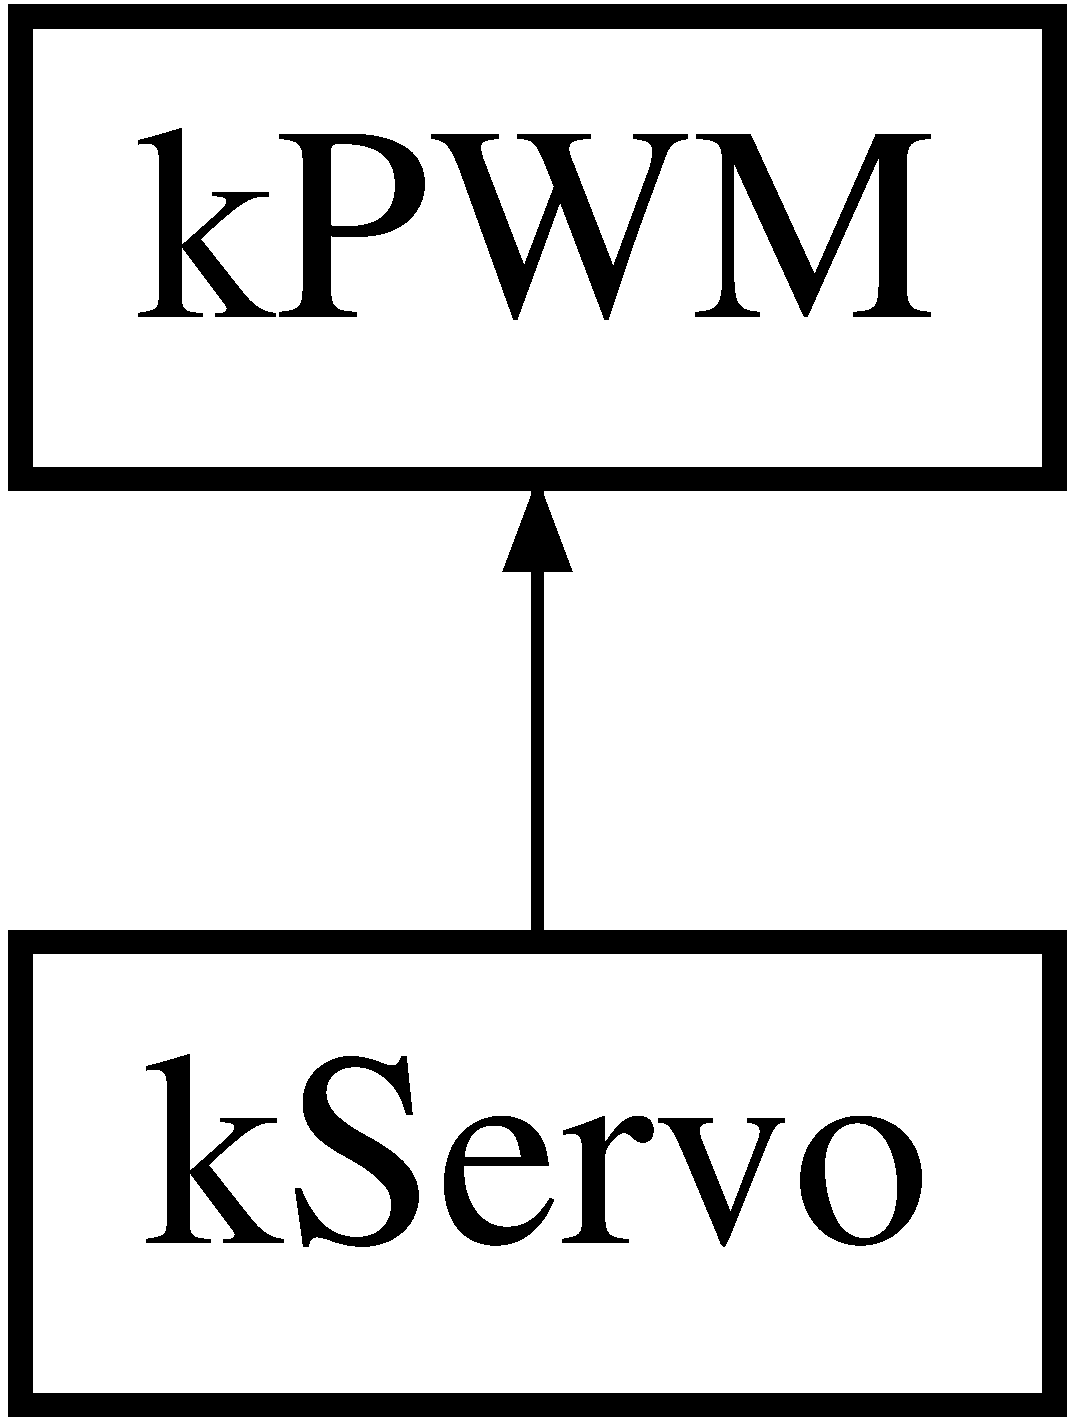
\includegraphics[height=2.000000cm]{classkPWM}
\end{center}
\end{figure}
\subsection*{Classes}
\begin{DoxyCompactItemize}
\item 
class \hyperlink{classkPWM_1_1kPWMHardware}{k\+P\+W\+M\+Hardware}
\end{DoxyCompactItemize}
\subsection*{Public Types}
\begin{DoxyCompactItemize}
\item 
enum {\bfseries k\+P\+W\+M\+\_\+\+Active\+State} \{ {\bfseries active\+High}, 
{\bfseries active\+Low}
 \}\hypertarget{classkPWM_a49e0da38cf214e3a0d52d6d511e71c39}{}\label{classkPWM_a49e0da38cf214e3a0d52d6d511e71c39}

\end{DoxyCompactItemize}
\subsection*{Public Member Functions}
\begin{DoxyCompactItemize}
\item 
void {\bfseries run} (unsigned short int resolution, unsigned int tick\+\_\+freq)\hypertarget{classkPWM_a0517e57ef741ed50402fa0bab8ae075e}{}\label{classkPWM_a0517e57ef741ed50402fa0bab8ae075e}

\item 
void {\bfseries operator=} (unsigned short int value)\hypertarget{classkPWM_a8ee0de783dbf27a60e3bed07740b516e}{}\label{classkPWM_a8ee0de783dbf27a60e3bed07740b516e}

\item 
{\bfseries operator unsigned int} ()\hypertarget{classkPWM_ac3114c91e72981e9e29e93d7899f87e5}{}\label{classkPWM_ac3114c91e72981e9e29e93d7899f87e5}

\end{DoxyCompactItemize}
\subsection*{Public Attributes}
\begin{DoxyCompactItemize}
\item 
\hyperlink{classkPWM_1_1kPWMHardware}{k\+P\+W\+M\+Hardware} {\bfseries hardware}\hypertarget{classkPWM_a66cc0314db7a2e743503aaf1f4dbc4b2}{}\label{classkPWM_a66cc0314db7a2e743503aaf1f4dbc4b2}

\end{DoxyCompactItemize}
\subsection*{Static Public Attributes}
\begin{DoxyCompactItemize}
\item 
static const \hyperlink{structkPWM__Timer1}{k\+P\+W\+M\+\_\+\+Timer1} $\ast$ {\bfseries Timer1} = (\hyperlink{structkPWM__Timer1}{k\+P\+W\+M\+\_\+\+Timer1} $\ast$)S\+R\+A\+M1\+\_\+\+B\+A\+SE\hypertarget{classkPWM_a04e0db3d7f1cbc7d06e89eed939b85cf}{}\label{classkPWM_a04e0db3d7f1cbc7d06e89eed939b85cf}

\item 
static const \hyperlink{structkPWM__Timer2}{k\+P\+W\+M\+\_\+\+Timer2} $\ast$ {\bfseries Timer2} = (\hyperlink{structkPWM__Timer2}{k\+P\+W\+M\+\_\+\+Timer2} $\ast$)S\+R\+A\+M1\+\_\+\+B\+A\+SE\hypertarget{classkPWM_ab30cc9d54138665c5b2d5f2790e9bdc7}{}\label{classkPWM_ab30cc9d54138665c5b2d5f2790e9bdc7}

\item 
static const \hyperlink{structkPWM__Timer3}{k\+P\+W\+M\+\_\+\+Timer3} $\ast$ {\bfseries Timer3} = (\hyperlink{structkPWM__Timer3}{k\+P\+W\+M\+\_\+\+Timer3} $\ast$)S\+R\+A\+M1\+\_\+\+B\+A\+SE\hypertarget{classkPWM_ab2ce1e6f24f870ec01adc7e1f3e963fc}{}\label{classkPWM_ab2ce1e6f24f870ec01adc7e1f3e963fc}

\item 
static const \hyperlink{structkPWM__Timer4}{k\+P\+W\+M\+\_\+\+Timer4} $\ast$ {\bfseries Timer4} = (\hyperlink{structkPWM__Timer4}{k\+P\+W\+M\+\_\+\+Timer4} $\ast$)S\+R\+A\+M1\+\_\+\+B\+A\+SE\hypertarget{classkPWM_a537d4a31158eb6320ed77615b539a088}{}\label{classkPWM_a537d4a31158eb6320ed77615b539a088}

\item 
static const \hyperlink{structkPWM__Timer5}{k\+P\+W\+M\+\_\+\+Timer5} $\ast$ {\bfseries Timer5} = (\hyperlink{structkPWM__Timer5}{k\+P\+W\+M\+\_\+\+Timer5} $\ast$)S\+R\+A\+M1\+\_\+\+B\+A\+SE\hypertarget{classkPWM_a8f94351d2b498ce8460d998b4845feb9}{}\label{classkPWM_a8f94351d2b498ce8460d998b4845feb9}

\item 
static const \hyperlink{structkPWM__Timer9}{k\+P\+W\+M\+\_\+\+Timer9} $\ast$ {\bfseries Timer9} = (\hyperlink{structkPWM__Timer9}{k\+P\+W\+M\+\_\+\+Timer9} $\ast$)S\+R\+A\+M1\+\_\+\+B\+A\+SE\hypertarget{classkPWM_a34727b8954262d0c9e74c51be8e02061}{}\label{classkPWM_a34727b8954262d0c9e74c51be8e02061}

\item 
static const \hyperlink{structkPWM__Timer10}{k\+P\+W\+M\+\_\+\+Timer10} $\ast$ {\bfseries Timer10} = (\hyperlink{structkPWM__Timer10}{k\+P\+W\+M\+\_\+\+Timer10} $\ast$)S\+R\+A\+M1\+\_\+\+B\+A\+SE\hypertarget{classkPWM_ac64472325767a9af8c24f18e0130dd33}{}\label{classkPWM_ac64472325767a9af8c24f18e0130dd33}

\item 
static const \hyperlink{structkPWM__Timer11}{k\+P\+W\+M\+\_\+\+Timer11} $\ast$ {\bfseries Timer11} = (\hyperlink{structkPWM__Timer11}{k\+P\+W\+M\+\_\+\+Timer11} $\ast$)S\+R\+A\+M1\+\_\+\+B\+A\+SE\hypertarget{classkPWM_af71367db3415ff7aa3581897e4fbb679}{}\label{classkPWM_af71367db3415ff7aa3581897e4fbb679}

\item 
static const \hyperlink{structkPWM__EXTI0}{k\+P\+W\+M\+\_\+\+E\+X\+T\+I0} $\ast$ {\bfseries E\+X\+T\+I0} = (\hyperlink{structkPWM__EXTI0}{k\+P\+W\+M\+\_\+\+E\+X\+T\+I0} $\ast$)S\+R\+A\+M1\+\_\+\+B\+A\+SE\hypertarget{classkPWM_a345f41328958a48fde4b02c0f1325fb7}{}\label{classkPWM_a345f41328958a48fde4b02c0f1325fb7}

\end{DoxyCompactItemize}


The documentation for this class was generated from the following files\+:\begin{DoxyCompactItemize}
\item 
k\+P\+W\+M.\+h\item 
k\+P\+W\+M.\+cpp\end{DoxyCompactItemize}

\hypertarget{structkPWM__EXTI0}{}\section{k\+P\+W\+M\+\_\+\+E\+X\+T\+I0 Struct Reference}
\label{structkPWM__EXTI0}\index{k\+P\+W\+M\+\_\+\+E\+X\+T\+I0@{k\+P\+W\+M\+\_\+\+E\+X\+T\+I0}}
\subsection*{Public Attributes}
\begin{DoxyCompactItemize}
\item 
\hyperlink{structkPWM__EXTI0__Pin}{k\+P\+W\+M\+\_\+\+E\+X\+T\+I0\+\_\+\+Pin} {\bfseries P\+O\+R\+T\+A0}\hypertarget{structkPWM__EXTI0_aa3a71d7f86dcf8a31fc502f18dc69fba}{}\label{structkPWM__EXTI0_aa3a71d7f86dcf8a31fc502f18dc69fba}

\item 
\hyperlink{structkPWM__EXTI0__Pin}{k\+P\+W\+M\+\_\+\+E\+X\+T\+I0\+\_\+\+Pin} {\bfseries P\+O\+R\+T\+B0}\hypertarget{structkPWM__EXTI0_aae513308957ac9d22ad880bad1dcdbe9}{}\label{structkPWM__EXTI0_aae513308957ac9d22ad880bad1dcdbe9}

\item 
\hyperlink{structkPWM__EXTI0__Pin}{k\+P\+W\+M\+\_\+\+E\+X\+T\+I0\+\_\+\+Pin} {\bfseries P\+O\+R\+T\+C0}\hypertarget{structkPWM__EXTI0_abf17bd93d09e5714d48e5762ef9b8d29}{}\label{structkPWM__EXTI0_abf17bd93d09e5714d48e5762ef9b8d29}

\item 
\hyperlink{structkPWM__EXTI0__Pin}{k\+P\+W\+M\+\_\+\+E\+X\+T\+I0\+\_\+\+Pin} {\bfseries P\+O\+R\+T\+D0}\hypertarget{structkPWM__EXTI0_a04eb86653c56e96aed7f69eda82ee72f}{}\label{structkPWM__EXTI0_a04eb86653c56e96aed7f69eda82ee72f}

\item 
\hyperlink{structkPWM__EXTI0__Pin}{k\+P\+W\+M\+\_\+\+E\+X\+T\+I0\+\_\+\+Pin} {\bfseries P\+O\+R\+T\+E0}\hypertarget{structkPWM__EXTI0_a5be32c8556f6de08ea9a1632d532e351}{}\label{structkPWM__EXTI0_a5be32c8556f6de08ea9a1632d532e351}

\item 
\hyperlink{structkPWM__EXTI0__Pin}{k\+P\+W\+M\+\_\+\+E\+X\+T\+I0\+\_\+\+Pin} {\bfseries P\+O\+R\+T\+F0}\hypertarget{structkPWM__EXTI0_a96672e3dad411bd52096e3f422b5405b}{}\label{structkPWM__EXTI0_a96672e3dad411bd52096e3f422b5405b}

\item 
\hyperlink{structkPWM__EXTI0__Pin}{k\+P\+W\+M\+\_\+\+E\+X\+T\+I0\+\_\+\+Pin} {\bfseries P\+O\+R\+T\+G0}\hypertarget{structkPWM__EXTI0_afaefd63c2035af4e6e7db55fc9daf331}{}\label{structkPWM__EXTI0_afaefd63c2035af4e6e7db55fc9daf331}

\end{DoxyCompactItemize}


The documentation for this struct was generated from the following file\+:\begin{DoxyCompactItemize}
\item 
k\+P\+W\+M.\+h\end{DoxyCompactItemize}

\hypertarget{structkPWM__EXTI0__Pin}{}\section{k\+P\+W\+M\+\_\+\+E\+X\+T\+I0\+\_\+\+Pin Struct Reference}
\label{structkPWM__EXTI0__Pin}\index{k\+P\+W\+M\+\_\+\+E\+X\+T\+I0\+\_\+\+Pin@{k\+P\+W\+M\+\_\+\+E\+X\+T\+I0\+\_\+\+Pin}}
\subsection*{Public Attributes}
\begin{DoxyCompactItemize}
\item 
unsigned char {\bfseries k\+P\+W\+M\+\_\+\+Pin}\hypertarget{structkPWM__EXTI0__Pin_a3ed1084a8325763f6a13bec108e4931f}{}\label{structkPWM__EXTI0__Pin_a3ed1084a8325763f6a13bec108e4931f}

\end{DoxyCompactItemize}


The documentation for this struct was generated from the following file\+:\begin{DoxyCompactItemize}
\item 
k\+P\+W\+M.\+h\end{DoxyCompactItemize}

\hypertarget{structkPWM__OC1__Timer1}{}\section{k\+P\+W\+M\+\_\+\+O\+C1\+\_\+\+Timer1 Struct Reference}
\label{structkPWM__OC1__Timer1}\index{k\+P\+W\+M\+\_\+\+O\+C1\+\_\+\+Timer1@{k\+P\+W\+M\+\_\+\+O\+C1\+\_\+\+Timer1}}
\subsection*{Public Attributes}
\begin{DoxyCompactItemize}
\item 
\hyperlink{structkPWM__Timer1Pin}{k\+P\+W\+M\+\_\+\+Timer1\+Pin} {\bfseries P\+O\+R\+T\+A8}\hypertarget{structkPWM__OC1__Timer1_a43ddb1c63fb26dc810f42ba5eca2faa7}{}\label{structkPWM__OC1__Timer1_a43ddb1c63fb26dc810f42ba5eca2faa7}

\item 
\hyperlink{structkPWM__Timer1Pin}{k\+P\+W\+M\+\_\+\+Timer1\+Pin} {\bfseries P\+O\+R\+T\+E9}\hypertarget{structkPWM__OC1__Timer1_aff413886fff4fae9a92684f5bb0723a2}{}\label{structkPWM__OC1__Timer1_aff413886fff4fae9a92684f5bb0723a2}

\end{DoxyCompactItemize}


The documentation for this struct was generated from the following file\+:\begin{DoxyCompactItemize}
\item 
k\+P\+W\+M.\+h\end{DoxyCompactItemize}

\hypertarget{structkPWM__OC1__Timer10}{}\section{k\+P\+W\+M\+\_\+\+O\+C1\+\_\+\+Timer10 Struct Reference}
\label{structkPWM__OC1__Timer10}\index{k\+P\+W\+M\+\_\+\+O\+C1\+\_\+\+Timer10@{k\+P\+W\+M\+\_\+\+O\+C1\+\_\+\+Timer10}}
\subsection*{Public Attributes}
\begin{DoxyCompactItemize}
\item 
\hyperlink{structkPWM__Timer10Pin}{k\+P\+W\+M\+\_\+\+Timer10\+Pin} {\bfseries P\+O\+R\+T\+B8}\hypertarget{structkPWM__OC1__Timer10_a60f35bb5d9228eac17ee7c2b7f4cd118}{}\label{structkPWM__OC1__Timer10_a60f35bb5d9228eac17ee7c2b7f4cd118}

\end{DoxyCompactItemize}


The documentation for this struct was generated from the following file\+:\begin{DoxyCompactItemize}
\item 
k\+P\+W\+M.\+h\end{DoxyCompactItemize}

\hypertarget{structkPWM__OC1__Timer11}{}\section{k\+P\+W\+M\+\_\+\+O\+C1\+\_\+\+Timer11 Struct Reference}
\label{structkPWM__OC1__Timer11}\index{k\+P\+W\+M\+\_\+\+O\+C1\+\_\+\+Timer11@{k\+P\+W\+M\+\_\+\+O\+C1\+\_\+\+Timer11}}
\subsection*{Public Attributes}
\begin{DoxyCompactItemize}
\item 
\hyperlink{structkPWM__Timer11Pin}{k\+P\+W\+M\+\_\+\+Timer11\+Pin} {\bfseries P\+O\+R\+T\+B9}\hypertarget{structkPWM__OC1__Timer11_a2018f287c3e8e52bcec85f434d521ba7}{}\label{structkPWM__OC1__Timer11_a2018f287c3e8e52bcec85f434d521ba7}

\end{DoxyCompactItemize}


The documentation for this struct was generated from the following file\+:\begin{DoxyCompactItemize}
\item 
k\+P\+W\+M.\+h\end{DoxyCompactItemize}

\hypertarget{structkPWM__OC1__Timer2}{}\section{k\+P\+W\+M\+\_\+\+O\+C1\+\_\+\+Timer2 Struct Reference}
\label{structkPWM__OC1__Timer2}\index{k\+P\+W\+M\+\_\+\+O\+C1\+\_\+\+Timer2@{k\+P\+W\+M\+\_\+\+O\+C1\+\_\+\+Timer2}}
\subsection*{Public Attributes}
\begin{DoxyCompactItemize}
\item 
\hyperlink{structkPWM__Timer2Pin}{k\+P\+W\+M\+\_\+\+Timer2\+Pin} {\bfseries P\+O\+R\+T\+A0}\hypertarget{structkPWM__OC1__Timer2_ab9ca88874e740b3e7ad5927b4bdc1544}{}\label{structkPWM__OC1__Timer2_ab9ca88874e740b3e7ad5927b4bdc1544}

\item 
\hyperlink{structkPWM__Timer2Pin}{k\+P\+W\+M\+\_\+\+Timer2\+Pin} {\bfseries P\+O\+R\+T\+A5}\hypertarget{structkPWM__OC1__Timer2_af5acd97823949654a98a90c4f1cd4928}{}\label{structkPWM__OC1__Timer2_af5acd97823949654a98a90c4f1cd4928}

\item 
\hyperlink{structkPWM__Timer2Pin}{k\+P\+W\+M\+\_\+\+Timer2\+Pin} {\bfseries P\+O\+R\+T\+A15}\hypertarget{structkPWM__OC1__Timer2_af025e443bca95684b3f01538470b44e4}{}\label{structkPWM__OC1__Timer2_af025e443bca95684b3f01538470b44e4}

\end{DoxyCompactItemize}


The documentation for this struct was generated from the following file\+:\begin{DoxyCompactItemize}
\item 
k\+P\+W\+M.\+h\end{DoxyCompactItemize}

\hypertarget{structkPWM__OC1__Timer3}{}\section{k\+P\+W\+M\+\_\+\+O\+C1\+\_\+\+Timer3 Struct Reference}
\label{structkPWM__OC1__Timer3}\index{k\+P\+W\+M\+\_\+\+O\+C1\+\_\+\+Timer3@{k\+P\+W\+M\+\_\+\+O\+C1\+\_\+\+Timer3}}
\subsection*{Public Attributes}
\begin{DoxyCompactItemize}
\item 
\hyperlink{structkPWM__Timer3Pin}{k\+P\+W\+M\+\_\+\+Timer3\+Pin} {\bfseries P\+O\+R\+T\+A6}\hypertarget{structkPWM__OC1__Timer3_a0422a77a6ea7b0bdf27ffc0c32ace4e5}{}\label{structkPWM__OC1__Timer3_a0422a77a6ea7b0bdf27ffc0c32ace4e5}

\item 
\hyperlink{structkPWM__Timer3Pin}{k\+P\+W\+M\+\_\+\+Timer3\+Pin} {\bfseries P\+O\+R\+T\+B4}\hypertarget{structkPWM__OC1__Timer3_a6f7c43a3cf0fe26b3ae8dbb68a8ca3da}{}\label{structkPWM__OC1__Timer3_a6f7c43a3cf0fe26b3ae8dbb68a8ca3da}

\item 
\hyperlink{structkPWM__Timer3Pin}{k\+P\+W\+M\+\_\+\+Timer3\+Pin} {\bfseries P\+O\+R\+T\+C6}\hypertarget{structkPWM__OC1__Timer3_a87fe6732418111fb1b5c8097d71f60e2}{}\label{structkPWM__OC1__Timer3_a87fe6732418111fb1b5c8097d71f60e2}

\end{DoxyCompactItemize}


The documentation for this struct was generated from the following file\+:\begin{DoxyCompactItemize}
\item 
k\+P\+W\+M.\+h\end{DoxyCompactItemize}

\hypertarget{structkPWM__OC1__Timer4}{}\section{k\+P\+W\+M\+\_\+\+O\+C1\+\_\+\+Timer4 Struct Reference}
\label{structkPWM__OC1__Timer4}\index{k\+P\+W\+M\+\_\+\+O\+C1\+\_\+\+Timer4@{k\+P\+W\+M\+\_\+\+O\+C1\+\_\+\+Timer4}}
\subsection*{Public Attributes}
\begin{DoxyCompactItemize}
\item 
\hyperlink{structkPWM__Timer4Pin}{k\+P\+W\+M\+\_\+\+Timer4\+Pin} {\bfseries P\+O\+R\+T\+B6}\hypertarget{structkPWM__OC1__Timer4_ab6964a95238638532b7fbe4775950ed8}{}\label{structkPWM__OC1__Timer4_ab6964a95238638532b7fbe4775950ed8}

\item 
\hyperlink{structkPWM__Timer4Pin}{k\+P\+W\+M\+\_\+\+Timer4\+Pin} {\bfseries P\+O\+R\+T\+D12}\hypertarget{structkPWM__OC1__Timer4_a57ccbd0b9ecedc0b838f80c4d45474d6}{}\label{structkPWM__OC1__Timer4_a57ccbd0b9ecedc0b838f80c4d45474d6}

\end{DoxyCompactItemize}


The documentation for this struct was generated from the following file\+:\begin{DoxyCompactItemize}
\item 
k\+P\+W\+M.\+h\end{DoxyCompactItemize}

\hypertarget{structkPWM__OC1__Timer5}{}\section{k\+P\+W\+M\+\_\+\+O\+C1\+\_\+\+Timer5 Struct Reference}
\label{structkPWM__OC1__Timer5}\index{k\+P\+W\+M\+\_\+\+O\+C1\+\_\+\+Timer5@{k\+P\+W\+M\+\_\+\+O\+C1\+\_\+\+Timer5}}
\subsection*{Public Attributes}
\begin{DoxyCompactItemize}
\item 
\hyperlink{structkPWM__Timer5Pin}{k\+P\+W\+M\+\_\+\+Timer5\+Pin} {\bfseries P\+O\+R\+T\+A0}\hypertarget{structkPWM__OC1__Timer5_aa13530c61dcc9b88cc0c3eb198fb8366}{}\label{structkPWM__OC1__Timer5_aa13530c61dcc9b88cc0c3eb198fb8366}

\end{DoxyCompactItemize}


The documentation for this struct was generated from the following file\+:\begin{DoxyCompactItemize}
\item 
k\+P\+W\+M.\+h\end{DoxyCompactItemize}

\hypertarget{structkPWM__OC1__Timer9}{}\section{k\+P\+W\+M\+\_\+\+O\+C1\+\_\+\+Timer9 Struct Reference}
\label{structkPWM__OC1__Timer9}\index{k\+P\+W\+M\+\_\+\+O\+C1\+\_\+\+Timer9@{k\+P\+W\+M\+\_\+\+O\+C1\+\_\+\+Timer9}}
\subsection*{Public Attributes}
\begin{DoxyCompactItemize}
\item 
\hyperlink{structkPWM__Timer9Pin}{k\+P\+W\+M\+\_\+\+Timer9\+Pin} {\bfseries P\+O\+R\+T\+A2}\hypertarget{structkPWM__OC1__Timer9_ad886508647968f6b905d89da39a17007}{}\label{structkPWM__OC1__Timer9_ad886508647968f6b905d89da39a17007}

\item 
\hyperlink{structkPWM__Timer9Pin}{k\+P\+W\+M\+\_\+\+Timer9\+Pin} {\bfseries P\+O\+R\+T\+E5}\hypertarget{structkPWM__OC1__Timer9_a7910ac894a5c9d1568c0347442fb6236}{}\label{structkPWM__OC1__Timer9_a7910ac894a5c9d1568c0347442fb6236}

\end{DoxyCompactItemize}


The documentation for this struct was generated from the following file\+:\begin{DoxyCompactItemize}
\item 
k\+P\+W\+M.\+h\end{DoxyCompactItemize}

\hypertarget{structkPWM__OC2__Timer1}{}\section{k\+P\+W\+M\+\_\+\+O\+C2\+\_\+\+Timer1 Struct Reference}
\label{structkPWM__OC2__Timer1}\index{k\+P\+W\+M\+\_\+\+O\+C2\+\_\+\+Timer1@{k\+P\+W\+M\+\_\+\+O\+C2\+\_\+\+Timer1}}
\subsection*{Public Attributes}
\begin{DoxyCompactItemize}
\item 
\hyperlink{structkPWM__Timer1Pin}{k\+P\+W\+M\+\_\+\+Timer1\+Pin} {\bfseries P\+O\+R\+T\+A9}\hypertarget{structkPWM__OC2__Timer1_acaaf02851260e197bc1601e7c6f1e176}{}\label{structkPWM__OC2__Timer1_acaaf02851260e197bc1601e7c6f1e176}

\item 
\hyperlink{structkPWM__Timer1Pin}{k\+P\+W\+M\+\_\+\+Timer1\+Pin} {\bfseries P\+O\+R\+T\+E11}\hypertarget{structkPWM__OC2__Timer1_aab064b59538ccb13d231f1bb9d3c9b65}{}\label{structkPWM__OC2__Timer1_aab064b59538ccb13d231f1bb9d3c9b65}

\end{DoxyCompactItemize}


The documentation for this struct was generated from the following file\+:\begin{DoxyCompactItemize}
\item 
k\+P\+W\+M.\+h\end{DoxyCompactItemize}

\hypertarget{structkPWM__OC2__Timer2}{}\section{k\+P\+W\+M\+\_\+\+O\+C2\+\_\+\+Timer2 Struct Reference}
\label{structkPWM__OC2__Timer2}\index{k\+P\+W\+M\+\_\+\+O\+C2\+\_\+\+Timer2@{k\+P\+W\+M\+\_\+\+O\+C2\+\_\+\+Timer2}}
\subsection*{Public Attributes}
\begin{DoxyCompactItemize}
\item 
\hyperlink{structkPWM__Timer2Pin}{k\+P\+W\+M\+\_\+\+Timer2\+Pin} {\bfseries P\+O\+R\+T\+A1}\hypertarget{structkPWM__OC2__Timer2_a284fd7ae8115124417293dc4713b4605}{}\label{structkPWM__OC2__Timer2_a284fd7ae8115124417293dc4713b4605}

\item 
\hyperlink{structkPWM__Timer2Pin}{k\+P\+W\+M\+\_\+\+Timer2\+Pin} {\bfseries P\+O\+R\+T\+B3}\hypertarget{structkPWM__OC2__Timer2_a1a9b06502c906ee5c5a78312452937e5}{}\label{structkPWM__OC2__Timer2_a1a9b06502c906ee5c5a78312452937e5}

\end{DoxyCompactItemize}


The documentation for this struct was generated from the following file\+:\begin{DoxyCompactItemize}
\item 
k\+P\+W\+M.\+h\end{DoxyCompactItemize}

\hypertarget{structkPWM__OC2__Timer3}{}\section{k\+P\+W\+M\+\_\+\+O\+C2\+\_\+\+Timer3 Struct Reference}
\label{structkPWM__OC2__Timer3}\index{k\+P\+W\+M\+\_\+\+O\+C2\+\_\+\+Timer3@{k\+P\+W\+M\+\_\+\+O\+C2\+\_\+\+Timer3}}
\subsection*{Public Attributes}
\begin{DoxyCompactItemize}
\item 
\hyperlink{structkPWM__Timer3Pin}{k\+P\+W\+M\+\_\+\+Timer3\+Pin} {\bfseries P\+O\+R\+T\+A7}\hypertarget{structkPWM__OC2__Timer3_a5275acf86aff80ba301c7ef653b28cbd}{}\label{structkPWM__OC2__Timer3_a5275acf86aff80ba301c7ef653b28cbd}

\item 
\hyperlink{structkPWM__Timer3Pin}{k\+P\+W\+M\+\_\+\+Timer3\+Pin} {\bfseries P\+O\+R\+T\+B5}\hypertarget{structkPWM__OC2__Timer3_af87ab6c0e540fe63488030e5a6d87614}{}\label{structkPWM__OC2__Timer3_af87ab6c0e540fe63488030e5a6d87614}

\item 
\hyperlink{structkPWM__Timer3Pin}{k\+P\+W\+M\+\_\+\+Timer3\+Pin} {\bfseries P\+O\+R\+T\+C7}\hypertarget{structkPWM__OC2__Timer3_aa17589b411aeb913ac3367c5f4ee119d}{}\label{structkPWM__OC2__Timer3_aa17589b411aeb913ac3367c5f4ee119d}

\end{DoxyCompactItemize}


The documentation for this struct was generated from the following file\+:\begin{DoxyCompactItemize}
\item 
k\+P\+W\+M.\+h\end{DoxyCompactItemize}

\hypertarget{structkPWM__OC2__Timer4}{}\section{k\+P\+W\+M\+\_\+\+O\+C2\+\_\+\+Timer4 Struct Reference}
\label{structkPWM__OC2__Timer4}\index{k\+P\+W\+M\+\_\+\+O\+C2\+\_\+\+Timer4@{k\+P\+W\+M\+\_\+\+O\+C2\+\_\+\+Timer4}}
\subsection*{Public Attributes}
\begin{DoxyCompactItemize}
\item 
\hyperlink{structkPWM__Timer4Pin}{k\+P\+W\+M\+\_\+\+Timer4\+Pin} {\bfseries P\+O\+R\+T\+B7}\hypertarget{structkPWM__OC2__Timer4_a776f178091d16ec27788c4dbe95b7762}{}\label{structkPWM__OC2__Timer4_a776f178091d16ec27788c4dbe95b7762}

\item 
\hyperlink{structkPWM__Timer4Pin}{k\+P\+W\+M\+\_\+\+Timer4\+Pin} {\bfseries P\+O\+R\+T\+D13}\hypertarget{structkPWM__OC2__Timer4_a31a68cfd9a8d73ed800f45a24f17e3ec}{}\label{structkPWM__OC2__Timer4_a31a68cfd9a8d73ed800f45a24f17e3ec}

\end{DoxyCompactItemize}


The documentation for this struct was generated from the following file\+:\begin{DoxyCompactItemize}
\item 
k\+P\+W\+M.\+h\end{DoxyCompactItemize}

\hypertarget{structkPWM__OC2__Timer5}{}\section{k\+P\+W\+M\+\_\+\+O\+C2\+\_\+\+Timer5 Struct Reference}
\label{structkPWM__OC2__Timer5}\index{k\+P\+W\+M\+\_\+\+O\+C2\+\_\+\+Timer5@{k\+P\+W\+M\+\_\+\+O\+C2\+\_\+\+Timer5}}
\subsection*{Public Attributes}
\begin{DoxyCompactItemize}
\item 
\hyperlink{structkPWM__Timer5Pin}{k\+P\+W\+M\+\_\+\+Timer5\+Pin} {\bfseries P\+O\+R\+T\+A1}\hypertarget{structkPWM__OC2__Timer5_a6971dd914847b55c5715957d97bb5e58}{}\label{structkPWM__OC2__Timer5_a6971dd914847b55c5715957d97bb5e58}

\end{DoxyCompactItemize}


The documentation for this struct was generated from the following file\+:\begin{DoxyCompactItemize}
\item 
k\+P\+W\+M.\+h\end{DoxyCompactItemize}

\hypertarget{structkPWM__OC2__Timer9}{}\section{k\+P\+W\+M\+\_\+\+O\+C2\+\_\+\+Timer9 Struct Reference}
\label{structkPWM__OC2__Timer9}\index{k\+P\+W\+M\+\_\+\+O\+C2\+\_\+\+Timer9@{k\+P\+W\+M\+\_\+\+O\+C2\+\_\+\+Timer9}}
\subsection*{Public Attributes}
\begin{DoxyCompactItemize}
\item 
\hyperlink{structkPWM__Timer9Pin}{k\+P\+W\+M\+\_\+\+Timer9\+Pin} {\bfseries P\+O\+R\+T\+A3}\hypertarget{structkPWM__OC2__Timer9_aedeb31c0da8e1aff0f39529c777186c1}{}\label{structkPWM__OC2__Timer9_aedeb31c0da8e1aff0f39529c777186c1}

\item 
\hyperlink{structkPWM__Timer9Pin}{k\+P\+W\+M\+\_\+\+Timer9\+Pin} {\bfseries P\+O\+R\+T\+E6}\hypertarget{structkPWM__OC2__Timer9_a5aba392fd17656a84c58429b1cd19c00}{}\label{structkPWM__OC2__Timer9_a5aba392fd17656a84c58429b1cd19c00}

\end{DoxyCompactItemize}


The documentation for this struct was generated from the following file\+:\begin{DoxyCompactItemize}
\item 
k\+P\+W\+M.\+h\end{DoxyCompactItemize}

\hypertarget{structkPWM__OC3__Timer1}{}\section{k\+P\+W\+M\+\_\+\+O\+C3\+\_\+\+Timer1 Struct Reference}
\label{structkPWM__OC3__Timer1}\index{k\+P\+W\+M\+\_\+\+O\+C3\+\_\+\+Timer1@{k\+P\+W\+M\+\_\+\+O\+C3\+\_\+\+Timer1}}
\subsection*{Public Attributes}
\begin{DoxyCompactItemize}
\item 
\hyperlink{structkPWM__Timer1Pin}{k\+P\+W\+M\+\_\+\+Timer1\+Pin} {\bfseries P\+O\+R\+T\+A10}\hypertarget{structkPWM__OC3__Timer1_a71e9afc19cfdf2eb66570d72c86d0fa3}{}\label{structkPWM__OC3__Timer1_a71e9afc19cfdf2eb66570d72c86d0fa3}

\item 
\hyperlink{structkPWM__Timer1Pin}{k\+P\+W\+M\+\_\+\+Timer1\+Pin} {\bfseries P\+O\+R\+T\+E13}\hypertarget{structkPWM__OC3__Timer1_a4f96044322a8b1251b4465024a5cc6bc}{}\label{structkPWM__OC3__Timer1_a4f96044322a8b1251b4465024a5cc6bc}

\end{DoxyCompactItemize}


The documentation for this struct was generated from the following file\+:\begin{DoxyCompactItemize}
\item 
k\+P\+W\+M.\+h\end{DoxyCompactItemize}

\hypertarget{structkPWM__OC3__Timer2}{}\section{k\+P\+W\+M\+\_\+\+O\+C3\+\_\+\+Timer2 Struct Reference}
\label{structkPWM__OC3__Timer2}\index{k\+P\+W\+M\+\_\+\+O\+C3\+\_\+\+Timer2@{k\+P\+W\+M\+\_\+\+O\+C3\+\_\+\+Timer2}}
\subsection*{Public Attributes}
\begin{DoxyCompactItemize}
\item 
\hyperlink{structkPWM__Timer2Pin}{k\+P\+W\+M\+\_\+\+Timer2\+Pin} {\bfseries P\+O\+R\+T\+A2}\hypertarget{structkPWM__OC3__Timer2_aebe91e1c8347e02c0a7d821ba0aca283}{}\label{structkPWM__OC3__Timer2_aebe91e1c8347e02c0a7d821ba0aca283}

\item 
\hyperlink{structkPWM__Timer2Pin}{k\+P\+W\+M\+\_\+\+Timer2\+Pin} {\bfseries P\+O\+R\+T\+B10}\hypertarget{structkPWM__OC3__Timer2_a22ec5c07d2dc71f62e8be05d9c728497}{}\label{structkPWM__OC3__Timer2_a22ec5c07d2dc71f62e8be05d9c728497}

\end{DoxyCompactItemize}


The documentation for this struct was generated from the following file\+:\begin{DoxyCompactItemize}
\item 
k\+P\+W\+M.\+h\end{DoxyCompactItemize}

\hypertarget{structkPWM__OC3__Timer3}{}\section{k\+P\+W\+M\+\_\+\+O\+C3\+\_\+\+Timer3 Struct Reference}
\label{structkPWM__OC3__Timer3}\index{k\+P\+W\+M\+\_\+\+O\+C3\+\_\+\+Timer3@{k\+P\+W\+M\+\_\+\+O\+C3\+\_\+\+Timer3}}
\subsection*{Public Attributes}
\begin{DoxyCompactItemize}
\item 
\hyperlink{structkPWM__Timer3Pin}{k\+P\+W\+M\+\_\+\+Timer3\+Pin} {\bfseries P\+O\+R\+T\+B0}\hypertarget{structkPWM__OC3__Timer3_a62c845e69156ef673b10f91dc332a8e6}{}\label{structkPWM__OC3__Timer3_a62c845e69156ef673b10f91dc332a8e6}

\item 
\hyperlink{structkPWM__Timer3Pin}{k\+P\+W\+M\+\_\+\+Timer3\+Pin} {\bfseries P\+O\+R\+T\+C8}\hypertarget{structkPWM__OC3__Timer3_a35a6ba1c3f34a730fe477e380148a256}{}\label{structkPWM__OC3__Timer3_a35a6ba1c3f34a730fe477e380148a256}

\end{DoxyCompactItemize}


The documentation for this struct was generated from the following file\+:\begin{DoxyCompactItemize}
\item 
k\+P\+W\+M.\+h\end{DoxyCompactItemize}

\hypertarget{structkPWM__OC3__Timer4}{}\section{k\+P\+W\+M\+\_\+\+O\+C3\+\_\+\+Timer4 Struct Reference}
\label{structkPWM__OC3__Timer4}\index{k\+P\+W\+M\+\_\+\+O\+C3\+\_\+\+Timer4@{k\+P\+W\+M\+\_\+\+O\+C3\+\_\+\+Timer4}}
\subsection*{Public Attributes}
\begin{DoxyCompactItemize}
\item 
\hyperlink{structkPWM__Timer4Pin}{k\+P\+W\+M\+\_\+\+Timer4\+Pin} {\bfseries P\+O\+R\+T\+B8}\hypertarget{structkPWM__OC3__Timer4_a4337819792f8ebdabce4a8560f59f52a}{}\label{structkPWM__OC3__Timer4_a4337819792f8ebdabce4a8560f59f52a}

\item 
\hyperlink{structkPWM__Timer4Pin}{k\+P\+W\+M\+\_\+\+Timer4\+Pin} {\bfseries P\+O\+R\+T\+D14}\hypertarget{structkPWM__OC3__Timer4_a23ceffe26f27b0f39ac81b00e3e4ae54}{}\label{structkPWM__OC3__Timer4_a23ceffe26f27b0f39ac81b00e3e4ae54}

\end{DoxyCompactItemize}


The documentation for this struct was generated from the following file\+:\begin{DoxyCompactItemize}
\item 
k\+P\+W\+M.\+h\end{DoxyCompactItemize}

\hypertarget{structkPWM__OC3__Timer5}{}\section{k\+P\+W\+M\+\_\+\+O\+C3\+\_\+\+Timer5 Struct Reference}
\label{structkPWM__OC3__Timer5}\index{k\+P\+W\+M\+\_\+\+O\+C3\+\_\+\+Timer5@{k\+P\+W\+M\+\_\+\+O\+C3\+\_\+\+Timer5}}
\subsection*{Public Attributes}
\begin{DoxyCompactItemize}
\item 
\hyperlink{structkPWM__Timer5Pin}{k\+P\+W\+M\+\_\+\+Timer5\+Pin} {\bfseries P\+O\+R\+T\+A2}\hypertarget{structkPWM__OC3__Timer5_a242e1a913b636907a55f56513106d855}{}\label{structkPWM__OC3__Timer5_a242e1a913b636907a55f56513106d855}

\end{DoxyCompactItemize}


The documentation for this struct was generated from the following file\+:\begin{DoxyCompactItemize}
\item 
k\+P\+W\+M.\+h\end{DoxyCompactItemize}

\hypertarget{structkPWM__OC4__Timer1}{}\section{k\+P\+W\+M\+\_\+\+O\+C4\+\_\+\+Timer1 Struct Reference}
\label{structkPWM__OC4__Timer1}\index{k\+P\+W\+M\+\_\+\+O\+C4\+\_\+\+Timer1@{k\+P\+W\+M\+\_\+\+O\+C4\+\_\+\+Timer1}}
\subsection*{Public Attributes}
\begin{DoxyCompactItemize}
\item 
\hyperlink{structkPWM__Timer1Pin}{k\+P\+W\+M\+\_\+\+Timer1\+Pin} {\bfseries P\+O\+R\+T\+A11}\hypertarget{structkPWM__OC4__Timer1_aca42e35f51af32f4669a931e84a3920d}{}\label{structkPWM__OC4__Timer1_aca42e35f51af32f4669a931e84a3920d}

\item 
\hyperlink{structkPWM__Timer1Pin}{k\+P\+W\+M\+\_\+\+Timer1\+Pin} {\bfseries P\+O\+R\+T\+E14}\hypertarget{structkPWM__OC4__Timer1_a9c1f74525b9a36fba14244fa03af8eba}{}\label{structkPWM__OC4__Timer1_a9c1f74525b9a36fba14244fa03af8eba}

\end{DoxyCompactItemize}


The documentation for this struct was generated from the following file\+:\begin{DoxyCompactItemize}
\item 
k\+P\+W\+M.\+h\end{DoxyCompactItemize}

\hypertarget{structkPWM__OC4__Timer2}{}\section{k\+P\+W\+M\+\_\+\+O\+C4\+\_\+\+Timer2 Struct Reference}
\label{structkPWM__OC4__Timer2}\index{k\+P\+W\+M\+\_\+\+O\+C4\+\_\+\+Timer2@{k\+P\+W\+M\+\_\+\+O\+C4\+\_\+\+Timer2}}
\subsection*{Public Attributes}
\begin{DoxyCompactItemize}
\item 
\hyperlink{structkPWM__Timer2Pin}{k\+P\+W\+M\+\_\+\+Timer2\+Pin} {\bfseries P\+O\+R\+T\+A3}\hypertarget{structkPWM__OC4__Timer2_aee3d8ffd5503012144683cd59bc68f1e}{}\label{structkPWM__OC4__Timer2_aee3d8ffd5503012144683cd59bc68f1e}

\item 
\hyperlink{structkPWM__Timer2Pin}{k\+P\+W\+M\+\_\+\+Timer2\+Pin} {\bfseries P\+O\+R\+T\+B11}\hypertarget{structkPWM__OC4__Timer2_a2f914c4ee986ef7ec358afcc117602d3}{}\label{structkPWM__OC4__Timer2_a2f914c4ee986ef7ec358afcc117602d3}

\end{DoxyCompactItemize}


The documentation for this struct was generated from the following file\+:\begin{DoxyCompactItemize}
\item 
k\+P\+W\+M.\+h\end{DoxyCompactItemize}

\hypertarget{structkPWM__OC4__Timer3}{}\section{k\+P\+W\+M\+\_\+\+O\+C4\+\_\+\+Timer3 Struct Reference}
\label{structkPWM__OC4__Timer3}\index{k\+P\+W\+M\+\_\+\+O\+C4\+\_\+\+Timer3@{k\+P\+W\+M\+\_\+\+O\+C4\+\_\+\+Timer3}}
\subsection*{Public Attributes}
\begin{DoxyCompactItemize}
\item 
\hyperlink{structkPWM__Timer3Pin}{k\+P\+W\+M\+\_\+\+Timer3\+Pin} {\bfseries P\+O\+R\+T\+B1}\hypertarget{structkPWM__OC4__Timer3_a53604d92f808755187ad498dd9c5b79e}{}\label{structkPWM__OC4__Timer3_a53604d92f808755187ad498dd9c5b79e}

\item 
\hyperlink{structkPWM__Timer3Pin}{k\+P\+W\+M\+\_\+\+Timer3\+Pin} {\bfseries P\+O\+R\+T\+C9}\hypertarget{structkPWM__OC4__Timer3_ace367036f62946381818851053b7d4c1}{}\label{structkPWM__OC4__Timer3_ace367036f62946381818851053b7d4c1}

\end{DoxyCompactItemize}


The documentation for this struct was generated from the following file\+:\begin{DoxyCompactItemize}
\item 
k\+P\+W\+M.\+h\end{DoxyCompactItemize}

\hypertarget{structkPWM__OC4__Timer4}{}\section{k\+P\+W\+M\+\_\+\+O\+C4\+\_\+\+Timer4 Struct Reference}
\label{structkPWM__OC4__Timer4}\index{k\+P\+W\+M\+\_\+\+O\+C4\+\_\+\+Timer4@{k\+P\+W\+M\+\_\+\+O\+C4\+\_\+\+Timer4}}
\subsection*{Public Attributes}
\begin{DoxyCompactItemize}
\item 
\hyperlink{structkPWM__Timer4Pin}{k\+P\+W\+M\+\_\+\+Timer4\+Pin} {\bfseries P\+O\+R\+T\+B9}\hypertarget{structkPWM__OC4__Timer4_a411f4d52c412a39507b0543bbc6187e1}{}\label{structkPWM__OC4__Timer4_a411f4d52c412a39507b0543bbc6187e1}

\item 
\hyperlink{structkPWM__Timer4Pin}{k\+P\+W\+M\+\_\+\+Timer4\+Pin} {\bfseries P\+O\+R\+T\+D15}\hypertarget{structkPWM__OC4__Timer4_a59d2dc1ef60f58f7236bcd3e3748aa7d}{}\label{structkPWM__OC4__Timer4_a59d2dc1ef60f58f7236bcd3e3748aa7d}

\end{DoxyCompactItemize}


The documentation for this struct was generated from the following file\+:\begin{DoxyCompactItemize}
\item 
k\+P\+W\+M.\+h\end{DoxyCompactItemize}

\hypertarget{structkPWM__OC4__Timer5}{}\section{k\+P\+W\+M\+\_\+\+O\+C4\+\_\+\+Timer5 Struct Reference}
\label{structkPWM__OC4__Timer5}\index{k\+P\+W\+M\+\_\+\+O\+C4\+\_\+\+Timer5@{k\+P\+W\+M\+\_\+\+O\+C4\+\_\+\+Timer5}}
\subsection*{Public Attributes}
\begin{DoxyCompactItemize}
\item 
\hyperlink{structkPWM__Timer5Pin}{k\+P\+W\+M\+\_\+\+Timer5\+Pin} {\bfseries P\+O\+R\+T\+A3}\hypertarget{structkPWM__OC4__Timer5_a14f0298a5755d50faa25dd39eceef8c2}{}\label{structkPWM__OC4__Timer5_a14f0298a5755d50faa25dd39eceef8c2}

\end{DoxyCompactItemize}


The documentation for this struct was generated from the following file\+:\begin{DoxyCompactItemize}
\item 
k\+P\+W\+M.\+h\end{DoxyCompactItemize}

\hypertarget{structkPWM__Timer1}{}\section{k\+P\+W\+M\+\_\+\+Timer1 Struct Reference}
\label{structkPWM__Timer1}\index{k\+P\+W\+M\+\_\+\+Timer1@{k\+P\+W\+M\+\_\+\+Timer1}}
\subsection*{Public Attributes}
\begin{DoxyCompactItemize}
\item 
\hyperlink{structkPWM__OC1__Timer1}{k\+P\+W\+M\+\_\+\+O\+C1\+\_\+\+Timer1} {\bfseries O\+C1}\hypertarget{structkPWM__Timer1_a4bc27acd77e6e6c59227e8b37298dec0}{}\label{structkPWM__Timer1_a4bc27acd77e6e6c59227e8b37298dec0}

\item 
\hyperlink{structkPWM__OC2__Timer1}{k\+P\+W\+M\+\_\+\+O\+C2\+\_\+\+Timer1} {\bfseries O\+C2}\hypertarget{structkPWM__Timer1_a4a59140c4452f5b409dd0cca362165a1}{}\label{structkPWM__Timer1_a4a59140c4452f5b409dd0cca362165a1}

\item 
\hyperlink{structkPWM__OC3__Timer1}{k\+P\+W\+M\+\_\+\+O\+C3\+\_\+\+Timer1} {\bfseries O\+C3}\hypertarget{structkPWM__Timer1_a5406942d01308b7832779673819d3caa}{}\label{structkPWM__Timer1_a5406942d01308b7832779673819d3caa}

\item 
\hyperlink{structkPWM__OC4__Timer1}{k\+P\+W\+M\+\_\+\+O\+C4\+\_\+\+Timer1} {\bfseries O\+C4}\hypertarget{structkPWM__Timer1_a39276ff1f4da23e14a86d9208d97802b}{}\label{structkPWM__Timer1_a39276ff1f4da23e14a86d9208d97802b}

\end{DoxyCompactItemize}


The documentation for this struct was generated from the following file\+:\begin{DoxyCompactItemize}
\item 
k\+P\+W\+M.\+h\end{DoxyCompactItemize}

\hypertarget{structkPWM__Timer10}{}\section{k\+P\+W\+M\+\_\+\+Timer10 Struct Reference}
\label{structkPWM__Timer10}\index{k\+P\+W\+M\+\_\+\+Timer10@{k\+P\+W\+M\+\_\+\+Timer10}}
\subsection*{Public Attributes}
\begin{DoxyCompactItemize}
\item 
\hyperlink{structkPWM__OC1__Timer10}{k\+P\+W\+M\+\_\+\+O\+C1\+\_\+\+Timer10} {\bfseries O\+C1}\hypertarget{structkPWM__Timer10_a017a65f4467820ad89be218cec9b8ad4}{}\label{structkPWM__Timer10_a017a65f4467820ad89be218cec9b8ad4}

\end{DoxyCompactItemize}


The documentation for this struct was generated from the following file\+:\begin{DoxyCompactItemize}
\item 
k\+P\+W\+M.\+h\end{DoxyCompactItemize}

\hypertarget{structkPWM__Timer10Pin}{}\section{k\+P\+W\+M\+\_\+\+Timer10\+Pin Struct Reference}
\label{structkPWM__Timer10Pin}\index{k\+P\+W\+M\+\_\+\+Timer10\+Pin@{k\+P\+W\+M\+\_\+\+Timer10\+Pin}}
\subsection*{Public Attributes}
\begin{DoxyCompactItemize}
\item 
unsigned char {\bfseries k\+P\+W\+M\+\_\+\+Pin}\hypertarget{structkPWM__Timer10Pin_a92dfb75ce6732f6b3bce71d46d5009eb}{}\label{structkPWM__Timer10Pin_a92dfb75ce6732f6b3bce71d46d5009eb}

\end{DoxyCompactItemize}


The documentation for this struct was generated from the following file\+:\begin{DoxyCompactItemize}
\item 
k\+P\+W\+M.\+h\end{DoxyCompactItemize}

\hypertarget{structkPWM__Timer11}{}\section{k\+P\+W\+M\+\_\+\+Timer11 Struct Reference}
\label{structkPWM__Timer11}\index{k\+P\+W\+M\+\_\+\+Timer11@{k\+P\+W\+M\+\_\+\+Timer11}}
\subsection*{Public Attributes}
\begin{DoxyCompactItemize}
\item 
\hyperlink{structkPWM__OC1__Timer11}{k\+P\+W\+M\+\_\+\+O\+C1\+\_\+\+Timer11} {\bfseries O\+C1}\hypertarget{structkPWM__Timer11_a949a837d3dee15e430a8e03ee5898c8d}{}\label{structkPWM__Timer11_a949a837d3dee15e430a8e03ee5898c8d}

\end{DoxyCompactItemize}


The documentation for this struct was generated from the following file\+:\begin{DoxyCompactItemize}
\item 
k\+P\+W\+M.\+h\end{DoxyCompactItemize}

\hypertarget{structkPWM__Timer11Pin}{}\section{k\+P\+W\+M\+\_\+\+Timer11\+Pin Struct Reference}
\label{structkPWM__Timer11Pin}\index{k\+P\+W\+M\+\_\+\+Timer11\+Pin@{k\+P\+W\+M\+\_\+\+Timer11\+Pin}}
\subsection*{Public Attributes}
\begin{DoxyCompactItemize}
\item 
unsigned char {\bfseries k\+P\+W\+M\+\_\+\+Pin}\hypertarget{structkPWM__Timer11Pin_aeeaf25f1b736edaa7784976ec1ec3b29}{}\label{structkPWM__Timer11Pin_aeeaf25f1b736edaa7784976ec1ec3b29}

\end{DoxyCompactItemize}


The documentation for this struct was generated from the following file\+:\begin{DoxyCompactItemize}
\item 
k\+P\+W\+M.\+h\end{DoxyCompactItemize}

\hypertarget{structkPWM__Timer1Pin}{}\section{k\+P\+W\+M\+\_\+\+Timer1\+Pin Struct Reference}
\label{structkPWM__Timer1Pin}\index{k\+P\+W\+M\+\_\+\+Timer1\+Pin@{k\+P\+W\+M\+\_\+\+Timer1\+Pin}}
\subsection*{Public Attributes}
\begin{DoxyCompactItemize}
\item 
unsigned char {\bfseries k\+P\+W\+M\+\_\+\+Pin}\hypertarget{structkPWM__Timer1Pin_a70bf1caebd445175377ea8e2d7f26f8b}{}\label{structkPWM__Timer1Pin_a70bf1caebd445175377ea8e2d7f26f8b}

\end{DoxyCompactItemize}


The documentation for this struct was generated from the following file\+:\begin{DoxyCompactItemize}
\item 
k\+P\+W\+M.\+h\end{DoxyCompactItemize}

\hypertarget{structkPWM__Timer2}{}\section{k\+P\+W\+M\+\_\+\+Timer2 Struct Reference}
\label{structkPWM__Timer2}\index{k\+P\+W\+M\+\_\+\+Timer2@{k\+P\+W\+M\+\_\+\+Timer2}}
\subsection*{Public Attributes}
\begin{DoxyCompactItemize}
\item 
\hyperlink{structkPWM__OC1__Timer2}{k\+P\+W\+M\+\_\+\+O\+C1\+\_\+\+Timer2} {\bfseries O\+C1}\hypertarget{structkPWM__Timer2_a020578e294b26b0704a0e2d452158db1}{}\label{structkPWM__Timer2_a020578e294b26b0704a0e2d452158db1}

\item 
\hyperlink{structkPWM__OC2__Timer2}{k\+P\+W\+M\+\_\+\+O\+C2\+\_\+\+Timer2} {\bfseries O\+C2}\hypertarget{structkPWM__Timer2_adba182e31dc7dd507a6402c03bdfc75a}{}\label{structkPWM__Timer2_adba182e31dc7dd507a6402c03bdfc75a}

\item 
\hyperlink{structkPWM__OC3__Timer2}{k\+P\+W\+M\+\_\+\+O\+C3\+\_\+\+Timer2} {\bfseries O\+C3}\hypertarget{structkPWM__Timer2_a7ac126db036b8752e89da4d8731f24cf}{}\label{structkPWM__Timer2_a7ac126db036b8752e89da4d8731f24cf}

\item 
\hyperlink{structkPWM__OC4__Timer2}{k\+P\+W\+M\+\_\+\+O\+C4\+\_\+\+Timer2} {\bfseries O\+C4}\hypertarget{structkPWM__Timer2_a71d50320eb03eeddcdb459cc8a4c28f0}{}\label{structkPWM__Timer2_a71d50320eb03eeddcdb459cc8a4c28f0}

\end{DoxyCompactItemize}


The documentation for this struct was generated from the following file\+:\begin{DoxyCompactItemize}
\item 
k\+P\+W\+M.\+h\end{DoxyCompactItemize}

\hypertarget{structkPWM__Timer2Pin}{}\section{k\+P\+W\+M\+\_\+\+Timer2\+Pin Struct Reference}
\label{structkPWM__Timer2Pin}\index{k\+P\+W\+M\+\_\+\+Timer2\+Pin@{k\+P\+W\+M\+\_\+\+Timer2\+Pin}}
\subsection*{Public Attributes}
\begin{DoxyCompactItemize}
\item 
unsigned char {\bfseries k\+P\+W\+M\+\_\+\+Pin}\hypertarget{structkPWM__Timer2Pin_abea76bb1d104ee3f7718c92d508ae89f}{}\label{structkPWM__Timer2Pin_abea76bb1d104ee3f7718c92d508ae89f}

\end{DoxyCompactItemize}


The documentation for this struct was generated from the following file\+:\begin{DoxyCompactItemize}
\item 
k\+P\+W\+M.\+h\end{DoxyCompactItemize}

\hypertarget{structkPWM__Timer3}{}\section{k\+P\+W\+M\+\_\+\+Timer3 Struct Reference}
\label{structkPWM__Timer3}\index{k\+P\+W\+M\+\_\+\+Timer3@{k\+P\+W\+M\+\_\+\+Timer3}}
\subsection*{Public Attributes}
\begin{DoxyCompactItemize}
\item 
\hyperlink{structkPWM__OC1__Timer3}{k\+P\+W\+M\+\_\+\+O\+C1\+\_\+\+Timer3} {\bfseries O\+C1}\hypertarget{structkPWM__Timer3_adc44e191488cea463df43ca7b5ef975c}{}\label{structkPWM__Timer3_adc44e191488cea463df43ca7b5ef975c}

\item 
\hyperlink{structkPWM__OC2__Timer3}{k\+P\+W\+M\+\_\+\+O\+C2\+\_\+\+Timer3} {\bfseries O\+C2}\hypertarget{structkPWM__Timer3_ac9cb2f2d977ee39e6f60395ea67d9c2b}{}\label{structkPWM__Timer3_ac9cb2f2d977ee39e6f60395ea67d9c2b}

\item 
\hyperlink{structkPWM__OC3__Timer3}{k\+P\+W\+M\+\_\+\+O\+C3\+\_\+\+Timer3} {\bfseries O\+C3}\hypertarget{structkPWM__Timer3_a7abed94bd83d89e92c16cea9ab67abed}{}\label{structkPWM__Timer3_a7abed94bd83d89e92c16cea9ab67abed}

\item 
\hyperlink{structkPWM__OC4__Timer3}{k\+P\+W\+M\+\_\+\+O\+C4\+\_\+\+Timer3} {\bfseries O\+C4}\hypertarget{structkPWM__Timer3_ad5b1744001490bada6f315da9903fb6e}{}\label{structkPWM__Timer3_ad5b1744001490bada6f315da9903fb6e}

\end{DoxyCompactItemize}


The documentation for this struct was generated from the following file\+:\begin{DoxyCompactItemize}
\item 
k\+P\+W\+M.\+h\end{DoxyCompactItemize}

\hypertarget{structkPWM__Timer3Pin}{}\section{k\+P\+W\+M\+\_\+\+Timer3\+Pin Struct Reference}
\label{structkPWM__Timer3Pin}\index{k\+P\+W\+M\+\_\+\+Timer3\+Pin@{k\+P\+W\+M\+\_\+\+Timer3\+Pin}}
\subsection*{Public Attributes}
\begin{DoxyCompactItemize}
\item 
unsigned char {\bfseries k\+P\+W\+M\+\_\+\+Pin}\hypertarget{structkPWM__Timer3Pin_aef573defa6b76fd6b1004ff39dd9691f}{}\label{structkPWM__Timer3Pin_aef573defa6b76fd6b1004ff39dd9691f}

\end{DoxyCompactItemize}


The documentation for this struct was generated from the following file\+:\begin{DoxyCompactItemize}
\item 
k\+P\+W\+M.\+h\end{DoxyCompactItemize}

\hypertarget{structkPWM__Timer4}{}\section{k\+P\+W\+M\+\_\+\+Timer4 Struct Reference}
\label{structkPWM__Timer4}\index{k\+P\+W\+M\+\_\+\+Timer4@{k\+P\+W\+M\+\_\+\+Timer4}}
\subsection*{Public Attributes}
\begin{DoxyCompactItemize}
\item 
\hyperlink{structkPWM__OC1__Timer4}{k\+P\+W\+M\+\_\+\+O\+C1\+\_\+\+Timer4} {\bfseries O\+C1}\hypertarget{structkPWM__Timer4_aa69aa9355e27a7b90a1450e8c7496a35}{}\label{structkPWM__Timer4_aa69aa9355e27a7b90a1450e8c7496a35}

\item 
\hyperlink{structkPWM__OC2__Timer4}{k\+P\+W\+M\+\_\+\+O\+C2\+\_\+\+Timer4} {\bfseries O\+C2}\hypertarget{structkPWM__Timer4_afcbadbab80c51faf963e1180f493d39a}{}\label{structkPWM__Timer4_afcbadbab80c51faf963e1180f493d39a}

\item 
\hyperlink{structkPWM__OC3__Timer4}{k\+P\+W\+M\+\_\+\+O\+C3\+\_\+\+Timer4} {\bfseries O\+C3}\hypertarget{structkPWM__Timer4_aea460129f5323c3989c069eebc673984}{}\label{structkPWM__Timer4_aea460129f5323c3989c069eebc673984}

\item 
\hyperlink{structkPWM__OC4__Timer4}{k\+P\+W\+M\+\_\+\+O\+C4\+\_\+\+Timer4} {\bfseries O\+C4}\hypertarget{structkPWM__Timer4_aa379ee76ef3ab2ace44790b985ee52a5}{}\label{structkPWM__Timer4_aa379ee76ef3ab2ace44790b985ee52a5}

\end{DoxyCompactItemize}


The documentation for this struct was generated from the following file\+:\begin{DoxyCompactItemize}
\item 
k\+P\+W\+M.\+h\end{DoxyCompactItemize}

\hypertarget{structkPWM__Timer4Pin}{}\section{k\+P\+W\+M\+\_\+\+Timer4\+Pin Struct Reference}
\label{structkPWM__Timer4Pin}\index{k\+P\+W\+M\+\_\+\+Timer4\+Pin@{k\+P\+W\+M\+\_\+\+Timer4\+Pin}}
\subsection*{Public Attributes}
\begin{DoxyCompactItemize}
\item 
unsigned char {\bfseries k\+P\+W\+M\+\_\+\+Pin}\hypertarget{structkPWM__Timer4Pin_a4f0a534af344928bc78842468b03d488}{}\label{structkPWM__Timer4Pin_a4f0a534af344928bc78842468b03d488}

\end{DoxyCompactItemize}


The documentation for this struct was generated from the following file\+:\begin{DoxyCompactItemize}
\item 
k\+P\+W\+M.\+h\end{DoxyCompactItemize}

\hypertarget{structkPWM__Timer5}{}\section{k\+P\+W\+M\+\_\+\+Timer5 Struct Reference}
\label{structkPWM__Timer5}\index{k\+P\+W\+M\+\_\+\+Timer5@{k\+P\+W\+M\+\_\+\+Timer5}}
\subsection*{Public Attributes}
\begin{DoxyCompactItemize}
\item 
\hyperlink{structkPWM__OC1__Timer5}{k\+P\+W\+M\+\_\+\+O\+C1\+\_\+\+Timer5} {\bfseries O\+C1}\hypertarget{structkPWM__Timer5_a24b1b3cc22a65991e00eb067f307dddd}{}\label{structkPWM__Timer5_a24b1b3cc22a65991e00eb067f307dddd}

\item 
\hyperlink{structkPWM__OC2__Timer5}{k\+P\+W\+M\+\_\+\+O\+C2\+\_\+\+Timer5} {\bfseries O\+C2}\hypertarget{structkPWM__Timer5_a68786f901586a82fbe8d5316b834f397}{}\label{structkPWM__Timer5_a68786f901586a82fbe8d5316b834f397}

\item 
\hyperlink{structkPWM__OC3__Timer5}{k\+P\+W\+M\+\_\+\+O\+C3\+\_\+\+Timer5} {\bfseries O\+C3}\hypertarget{structkPWM__Timer5_a90c677409a408f98bba85592bbfb38fe}{}\label{structkPWM__Timer5_a90c677409a408f98bba85592bbfb38fe}

\item 
\hyperlink{structkPWM__OC4__Timer5}{k\+P\+W\+M\+\_\+\+O\+C4\+\_\+\+Timer5} {\bfseries O\+C4}\hypertarget{structkPWM__Timer5_a40ad871d2dad8083110273e14384f2be}{}\label{structkPWM__Timer5_a40ad871d2dad8083110273e14384f2be}

\end{DoxyCompactItemize}


The documentation for this struct was generated from the following file\+:\begin{DoxyCompactItemize}
\item 
k\+P\+W\+M.\+h\end{DoxyCompactItemize}

\hypertarget{structkPWM__Timer5Pin}{}\section{k\+P\+W\+M\+\_\+\+Timer5\+Pin Struct Reference}
\label{structkPWM__Timer5Pin}\index{k\+P\+W\+M\+\_\+\+Timer5\+Pin@{k\+P\+W\+M\+\_\+\+Timer5\+Pin}}
\subsection*{Public Attributes}
\begin{DoxyCompactItemize}
\item 
unsigned char {\bfseries k\+P\+W\+M\+\_\+\+Pin}\hypertarget{structkPWM__Timer5Pin_a1620a72e3e6ee5d140aa0d3267ca9807}{}\label{structkPWM__Timer5Pin_a1620a72e3e6ee5d140aa0d3267ca9807}

\end{DoxyCompactItemize}


The documentation for this struct was generated from the following file\+:\begin{DoxyCompactItemize}
\item 
k\+P\+W\+M.\+h\end{DoxyCompactItemize}

\hypertarget{structkPWM__Timer9}{}\section{k\+P\+W\+M\+\_\+\+Timer9 Struct Reference}
\label{structkPWM__Timer9}\index{k\+P\+W\+M\+\_\+\+Timer9@{k\+P\+W\+M\+\_\+\+Timer9}}
\subsection*{Public Attributes}
\begin{DoxyCompactItemize}
\item 
\hyperlink{structkPWM__OC1__Timer9}{k\+P\+W\+M\+\_\+\+O\+C1\+\_\+\+Timer9} {\bfseries O\+C1}\hypertarget{structkPWM__Timer9_ac48aad158b7e4f6b8791bcf8b239185d}{}\label{structkPWM__Timer9_ac48aad158b7e4f6b8791bcf8b239185d}

\item 
\hyperlink{structkPWM__OC2__Timer9}{k\+P\+W\+M\+\_\+\+O\+C2\+\_\+\+Timer9} {\bfseries O\+C2}\hypertarget{structkPWM__Timer9_a8d7aeb4c69bd79c3b266126886f572f3}{}\label{structkPWM__Timer9_a8d7aeb4c69bd79c3b266126886f572f3}

\end{DoxyCompactItemize}


The documentation for this struct was generated from the following file\+:\begin{DoxyCompactItemize}
\item 
k\+P\+W\+M.\+h\end{DoxyCompactItemize}

\hypertarget{structkPWM__Timer9Pin}{}\section{k\+P\+W\+M\+\_\+\+Timer9\+Pin Struct Reference}
\label{structkPWM__Timer9Pin}\index{k\+P\+W\+M\+\_\+\+Timer9\+Pin@{k\+P\+W\+M\+\_\+\+Timer9\+Pin}}
\subsection*{Public Attributes}
\begin{DoxyCompactItemize}
\item 
unsigned char {\bfseries k\+P\+W\+M\+\_\+\+Pin}\hypertarget{structkPWM__Timer9Pin_ad701a39ac4991cd1d4ed7c7bb3d8c724}{}\label{structkPWM__Timer9Pin_ad701a39ac4991cd1d4ed7c7bb3d8c724}

\end{DoxyCompactItemize}


The documentation for this struct was generated from the following file\+:\begin{DoxyCompactItemize}
\item 
k\+P\+W\+M.\+h\end{DoxyCompactItemize}

\hypertarget{classkPWM_1_1kPWMHardware}{}\section{k\+P\+WM\+:\+:k\+P\+W\+M\+Hardware Class Reference}
\label{classkPWM_1_1kPWMHardware}\index{k\+P\+W\+M\+::k\+P\+W\+M\+Hardware@{k\+P\+W\+M\+::k\+P\+W\+M\+Hardware}}
\subsection*{Public Member Functions}
\begin{DoxyCompactItemize}
\item 
\hyperlink{classkPWM_1_1kPWMHardware}{k\+P\+W\+M\+Hardware} \& {\bfseries operator=} (const \hyperlink{structkPWM__Timer2Pin}{k\+P\+W\+M\+\_\+\+Timer2\+Pin} \&pwm\+Hard)\hypertarget{classkPWM_1_1kPWMHardware_acb4fbda01dac038bf5dfca605dfab0ef}{}\label{classkPWM_1_1kPWMHardware_acb4fbda01dac038bf5dfca605dfab0ef}

\item 
\hyperlink{classkPWM_1_1kPWMHardware}{k\+P\+W\+M\+Hardware} \& {\bfseries operator=} (const \hyperlink{structkPWM__Timer1Pin}{k\+P\+W\+M\+\_\+\+Timer1\+Pin} \&pwm\+Hard)\hypertarget{classkPWM_1_1kPWMHardware_abca1d455a282789e17966d90934f73ef}{}\label{classkPWM_1_1kPWMHardware_abca1d455a282789e17966d90934f73ef}

\item 
\hyperlink{classkPWM_1_1kPWMHardware}{k\+P\+W\+M\+Hardware} \& {\bfseries operator=} (const \hyperlink{structkPWM__Timer3Pin}{k\+P\+W\+M\+\_\+\+Timer3\+Pin} \&pwm\+Hard)\hypertarget{classkPWM_1_1kPWMHardware_af058989fe3c27a15315764f353ce195b}{}\label{classkPWM_1_1kPWMHardware_af058989fe3c27a15315764f353ce195b}

\item 
\hyperlink{classkPWM_1_1kPWMHardware}{k\+P\+W\+M\+Hardware} \& {\bfseries operator=} (const \hyperlink{structkPWM__Timer4Pin}{k\+P\+W\+M\+\_\+\+Timer4\+Pin} \&pwm\+Hard)\hypertarget{classkPWM_1_1kPWMHardware_aea1806117cf165398e6664a3413d2107}{}\label{classkPWM_1_1kPWMHardware_aea1806117cf165398e6664a3413d2107}

\item 
\hyperlink{classkPWM_1_1kPWMHardware}{k\+P\+W\+M\+Hardware} \& {\bfseries operator=} (const \hyperlink{structkPWM__Timer5Pin}{k\+P\+W\+M\+\_\+\+Timer5\+Pin} \&pwm\+Hard)\hypertarget{classkPWM_1_1kPWMHardware_a496e6d4d882369ddf5069842f4e0364e}{}\label{classkPWM_1_1kPWMHardware_a496e6d4d882369ddf5069842f4e0364e}

\item 
\hyperlink{classkPWM_1_1kPWMHardware}{k\+P\+W\+M\+Hardware} \& {\bfseries operator=} (const \hyperlink{structkPWM__Timer9Pin}{k\+P\+W\+M\+\_\+\+Timer9\+Pin} \&pwm\+Hard)\hypertarget{classkPWM_1_1kPWMHardware_a919592a44da54464e729537839bbd95b}{}\label{classkPWM_1_1kPWMHardware_a919592a44da54464e729537839bbd95b}

\item 
\hyperlink{classkPWM_1_1kPWMHardware}{k\+P\+W\+M\+Hardware} \& {\bfseries operator=} (const \hyperlink{structkPWM__Timer10Pin}{k\+P\+W\+M\+\_\+\+Timer10\+Pin} \&pwm\+Hard)\hypertarget{classkPWM_1_1kPWMHardware_a9ccf3def0e1eb585dfed27d2e4f5a2f7}{}\label{classkPWM_1_1kPWMHardware_a9ccf3def0e1eb585dfed27d2e4f5a2f7}

\item 
\hyperlink{classkPWM_1_1kPWMHardware}{k\+P\+W\+M\+Hardware} \& {\bfseries operator=} (const \hyperlink{structkPWM__Timer11Pin}{k\+P\+W\+M\+\_\+\+Timer11\+Pin} \&pwm\+Hard)\hypertarget{classkPWM_1_1kPWMHardware_a3116709156c3905e8cc6f19a87fec76f}{}\label{classkPWM_1_1kPWMHardware_a3116709156c3905e8cc6f19a87fec76f}

\item 
\hyperlink{classkPWM_1_1kPWMHardware}{k\+P\+W\+M\+Hardware} \& {\bfseries operator=} (const k\+P\+W\+M\+::k\+P\+W\+M\+\_\+\+Active\+State state)\hypertarget{classkPWM_1_1kPWMHardware_a8b52bc1d5f06fcb6152629ac88741372}{}\label{classkPWM_1_1kPWMHardware_a8b52bc1d5f06fcb6152629ac88741372}

\item 
\hyperlink{classkPWM_1_1kPWMHardware}{k\+P\+W\+M\+Hardware} \& {\bfseries operator=} (const \hyperlink{structkPWM__EXTI0__Pin}{k\+P\+W\+M\+\_\+\+E\+X\+T\+I0\+\_\+\+Pin} \&pwm\+Hard)\hypertarget{classkPWM_1_1kPWMHardware_adc259bf9925d9c809b50d761751a7d38}{}\label{classkPWM_1_1kPWMHardware_adc259bf9925d9c809b50d761751a7d38}

\end{DoxyCompactItemize}
\subsection*{Public Attributes}
\begin{DoxyCompactItemize}
\item 
T\+I\+M\+\_\+\+Type\+Def $\ast$ {\bfseries tim}\hypertarget{classkPWM_1_1kPWMHardware_a5452e7cf3462cfd59e1fff29575b503c}{}\label{classkPWM_1_1kPWMHardware_a5452e7cf3462cfd59e1fff29575b503c}

\item 
uint32\+\_\+t $\ast$ {\bfseries output}\hypertarget{classkPWM_1_1kPWMHardware_ac688787abc9ee29b8d4c6b2e9f798159}{}\label{classkPWM_1_1kPWMHardware_ac688787abc9ee29b8d4c6b2e9f798159}

\item 
uint32\+\_\+t {\bfseries input}\hypertarget{classkPWM_1_1kPWMHardware_a3107a8671ec1e9f8fe6ed1e2aa262203}{}\label{classkPWM_1_1kPWMHardware_a3107a8671ec1e9f8fe6ed1e2aa262203}

\end{DoxyCompactItemize}


The documentation for this class was generated from the following files\+:\begin{DoxyCompactItemize}
\item 
k\+P\+W\+M.\+h\item 
k\+P\+W\+M.\+cpp\end{DoxyCompactItemize}

\hypertarget{classkQuaternion}{}\section{k\+Quaternion Class Reference}
\label{classkQuaternion}\index{k\+Quaternion@{k\+Quaternion}}
\subsection*{Public Member Functions}
\begin{DoxyCompactItemize}
\item 
void {\bfseries operator+=} (\hyperlink{classkQuaternion}{k\+Quaternion} \&q)\hypertarget{classkQuaternion_ad7cdf002b65f3b8834bc63d45085daaf}{}\label{classkQuaternion_ad7cdf002b65f3b8834bc63d45085daaf}

\item 
void {\bfseries operator-\/=} (\hyperlink{classkQuaternion}{k\+Quaternion} \&q)\hypertarget{classkQuaternion_ad119145d9e5026251501bd6e41aaa456}{}\label{classkQuaternion_ad119145d9e5026251501bd6e41aaa456}

\item 
void {\bfseries operator$\ast$=} (\hyperlink{classkQuaternion}{k\+Quaternion} \&q)\hypertarget{classkQuaternion_a094cdffdf4501a2e00020ffcc6e83765}{}\label{classkQuaternion_a094cdffdf4501a2e00020ffcc6e83765}

\item 
void {\bfseries operator$\ast$=} (float \&scalar)\hypertarget{classkQuaternion_abc194ebc9421ccd3f901a5121ce6fae0}{}\label{classkQuaternion_abc194ebc9421ccd3f901a5121ce6fae0}

\item 
\hyperlink{classkQuaternion}{k\+Quaternion} {\bfseries operator$\ast$} (\hyperlink{classkQuaternion}{k\+Quaternion} \&q)\hypertarget{classkQuaternion_ae3b067edd24a80b63e4bc9d2e2732f5a}{}\label{classkQuaternion_ae3b067edd24a80b63e4bc9d2e2732f5a}

\item 
\hyperlink{classkQuaternion}{k\+Quaternion} {\bfseries operator+} (\hyperlink{classkQuaternion}{k\+Quaternion} \&q)\hypertarget{classkQuaternion_ac2c240c40856d85c97643698814a4a4c}{}\label{classkQuaternion_ac2c240c40856d85c97643698814a4a4c}

\item 
\hyperlink{classkQuaternion}{k\+Quaternion} {\bfseries operator-\/} (\hyperlink{classkQuaternion}{k\+Quaternion} \&q)\hypertarget{classkQuaternion_ad3df490cbd3c7e4a435f7b7abfa80bf0}{}\label{classkQuaternion_ad3df490cbd3c7e4a435f7b7abfa80bf0}

\item 
void {\bfseries operator=} (\hyperlink{classkQuaternion}{k\+Quaternion} \&q)\hypertarget{classkQuaternion_a02340df8aec8392a17fa6644be34a360}{}\label{classkQuaternion_a02340df8aec8392a17fa6644be34a360}

\item 
bool {\bfseries operator==} (\hyperlink{classkQuaternion}{k\+Quaternion} \&q)\hypertarget{classkQuaternion_a0d2571c18862c02bd36cbdabc3d15af7}{}\label{classkQuaternion_a0d2571c18862c02bd36cbdabc3d15af7}

\item 
float {\bfseries norm} (void)\hypertarget{classkQuaternion_ab82936e9305a3f4ccc4b2c595881c5da}{}\label{classkQuaternion_ab82936e9305a3f4ccc4b2c595881c5da}

\item 
\hyperlink{classkQuaternion}{k\+Quaternion} {\bfseries inv} (void)\hypertarget{classkQuaternion_aa1fda1494a4c8a0321c072c1510eb0c5}{}\label{classkQuaternion_aa1fda1494a4c8a0321c072c1510eb0c5}

\item 
\hyperlink{classkQuaternion}{k\+Quaternion} {\bfseries versor} (void)\hypertarget{classkQuaternion_a4a04dbc061679cc2cf4241de361cfd6f}{}\label{classkQuaternion_a4a04dbc061679cc2cf4241de361cfd6f}

\item 
\hyperlink{classkQuaternion}{k\+Quaternion} {\bfseries conjugate} (void)\hypertarget{classkQuaternion_ac6499af96761a4fc5afac3cf62a387fb}{}\label{classkQuaternion_ac6499af96761a4fc5afac3cf62a387fb}

\item 
\hyperlink{classkQuaternion}{k\+Quaternion} {\bfseries reciprocal} (void)\hypertarget{classkQuaternion_a2d17d3d7eee3809f3aec59bd6e3fefc4}{}\label{classkQuaternion_a2d17d3d7eee3809f3aec59bd6e3fefc4}

\end{DoxyCompactItemize}
\subsection*{Public Attributes}
\begin{DoxyCompactItemize}
\item 
float {\bfseries r}\hypertarget{classkQuaternion_a856e152179f6116a478b2650064fa0de}{}\label{classkQuaternion_a856e152179f6116a478b2650064fa0de}

\item 
float {\bfseries i}\hypertarget{classkQuaternion_a26ff17e9921a568a83658bedf62d0d40}{}\label{classkQuaternion_a26ff17e9921a568a83658bedf62d0d40}

\item 
float {\bfseries j}\hypertarget{classkQuaternion_a7a9a190b543fc248017d43c50f3cff6e}{}\label{classkQuaternion_a7a9a190b543fc248017d43c50f3cff6e}

\item 
float {\bfseries k}\hypertarget{classkQuaternion_a42ca54ef4737cae765625a68e5ee0983}{}\label{classkQuaternion_a42ca54ef4737cae765625a68e5ee0983}

\end{DoxyCompactItemize}


The documentation for this class was generated from the following files\+:\begin{DoxyCompactItemize}
\item 
k\+Quaternion.\+h\item 
k\+Quaternion.\+cpp\end{DoxyCompactItemize}

\hypertarget{classkSDCard}{}\section{k\+S\+D\+Card Class Reference}
\label{classkSDCard}\index{k\+S\+D\+Card@{k\+S\+D\+Card}}
Inheritance diagram for k\+S\+D\+Card\+:\begin{figure}[H]
\begin{center}
\leavevmode
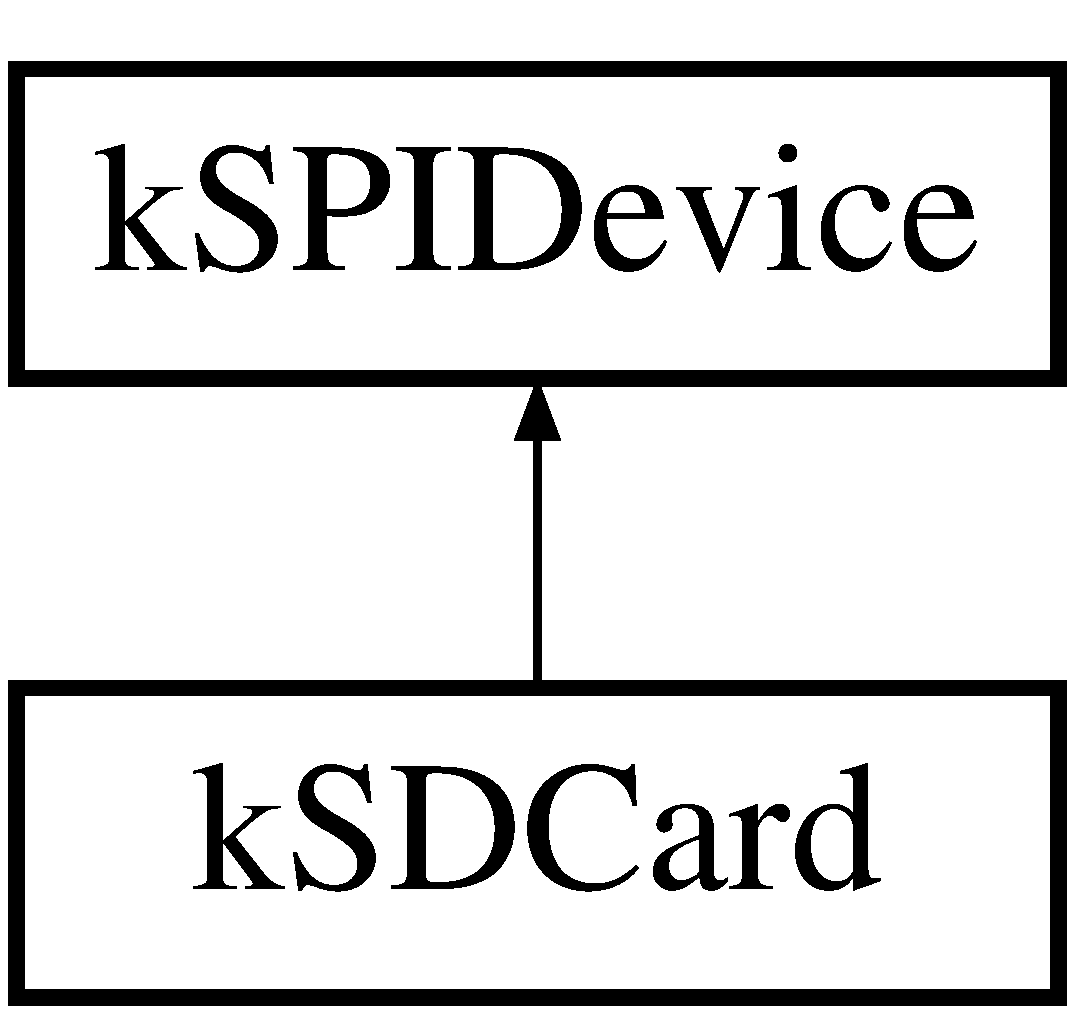
\includegraphics[height=2.000000cm]{classkSDCard}
\end{center}
\end{figure}
\subsection*{Public Member Functions}
\begin{DoxyCompactItemize}
\item 
unsigned char {\bfseries init} (void)\hypertarget{classkSDCard_a09af8bfa22e0e4f4c62ae38b14a5842e}{}\label{classkSDCard_a09af8bfa22e0e4f4c62ae38b14a5842e}

\item 
unsigned char {\bfseries mounted} (void)\hypertarget{classkSDCard_a6e9f64bf6068b7e58b539e7bbcaa03d2}{}\label{classkSDCard_a6e9f64bf6068b7e58b539e7bbcaa03d2}

\item 
unsigned char {\bfseries send\+C\+MD} (unsigned char cmd, unsigned int arg)\hypertarget{classkSDCard_a91c717f5da5833e685325bdd41cbba1f}{}\label{classkSDCard_a91c717f5da5833e685325bdd41cbba1f}

\end{DoxyCompactItemize}
\subsection*{Additional Inherited Members}


The documentation for this class was generated from the following files\+:\begin{DoxyCompactItemize}
\item 
k\+S\+D\+Card.\+h\item 
k\+S\+D\+Card.\+cpp\end{DoxyCompactItemize}

\hypertarget{classkSerial}{}\section{k\+Serial Class Reference}
\label{classkSerial}\index{k\+Serial@{k\+Serial}}
Inheritance diagram for k\+Serial\+:\begin{figure}[H]
\begin{center}
\leavevmode
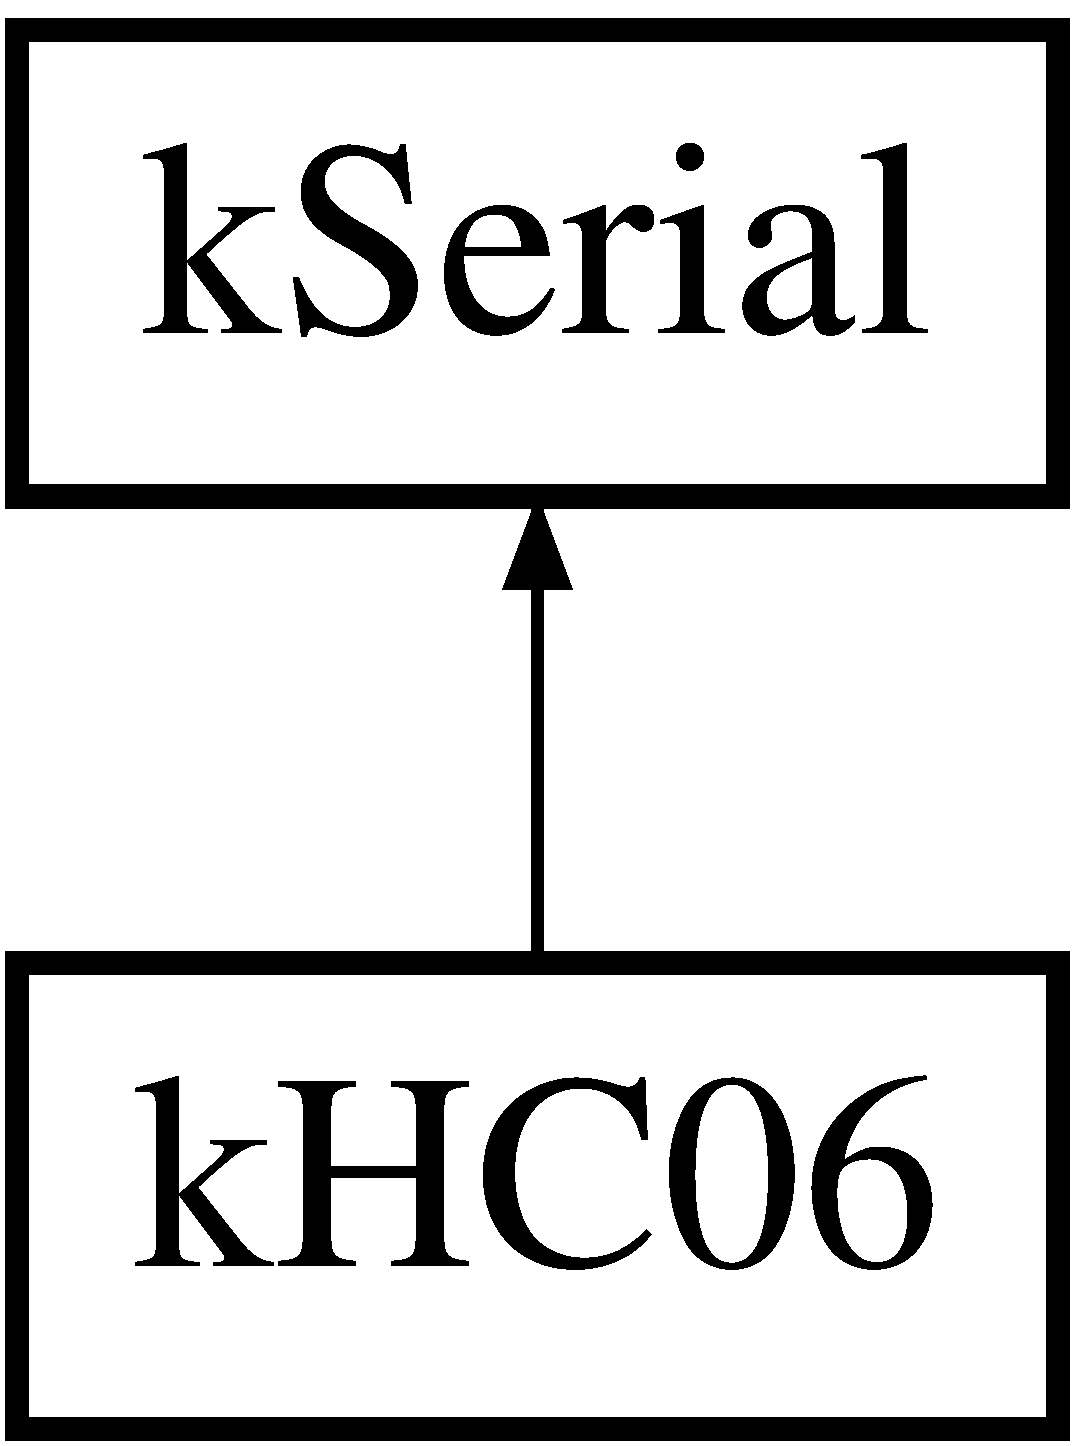
\includegraphics[height=2.000000cm]{classkSerial}
\end{center}
\end{figure}
\subsection*{Public Member Functions}
\begin{DoxyCompactItemize}
\item 
{\bfseries k\+Serial} (const \hyperlink{classkSerial}{k\+Serial} \&other)\hypertarget{classkSerial_a502c455e261a0121bf5e2671bec75589}{}\label{classkSerial_a502c455e261a0121bf5e2671bec75589}

\item 
{\bfseries k\+Serial} (const \hyperlink{structkSerialUSART1Pin}{k\+Serial\+U\+S\+A\+R\+T1\+Pin} \&Rx, const \hyperlink{structkSerialUSART1Pin}{k\+Serial\+U\+S\+A\+R\+T1\+Pin} \&Tx, unsigned int Baud\+Rate)\hypertarget{classkSerial_a0d01a0ca232842283d6e74dc1aade899}{}\label{classkSerial_a0d01a0ca232842283d6e74dc1aade899}

\item 
{\bfseries k\+Serial} (const \hyperlink{structkSerialUSART1Pin}{k\+Serial\+U\+S\+A\+R\+T1\+Pin} \&Pin, unsigned int Baud\+Rate)\hypertarget{classkSerial_a5147a9eaac433e07017e382cd2244972}{}\label{classkSerial_a5147a9eaac433e07017e382cd2244972}

\item 
{\bfseries k\+Serial} (const \hyperlink{structkSerialUSART2Pin}{k\+Serial\+U\+S\+A\+R\+T2\+Pin} \&Rx, const \hyperlink{structkSerialUSART2Pin}{k\+Serial\+U\+S\+A\+R\+T2\+Pin} \&Tx, unsigned int Baud\+Rate)\hypertarget{classkSerial_a5ce28ad3c00c5eb60110e0037e3d6025}{}\label{classkSerial_a5ce28ad3c00c5eb60110e0037e3d6025}

\item 
{\bfseries k\+Serial} (const \hyperlink{structkSerialUSART2Pin}{k\+Serial\+U\+S\+A\+R\+T2\+Pin} \&Pin, unsigned int Baud\+Rate)\hypertarget{classkSerial_aff7fb8ae9ba68ef546065f73d7168bae}{}\label{classkSerial_aff7fb8ae9ba68ef546065f73d7168bae}

\item 
{\bfseries k\+Serial} (const \hyperlink{structkSerialUSART3Pin}{k\+Serial\+U\+S\+A\+R\+T3\+Pin} \&Rx, const \hyperlink{structkSerialUSART3Pin}{k\+Serial\+U\+S\+A\+R\+T3\+Pin} \&Tx, unsigned int Baud\+Rate)\hypertarget{classkSerial_a95e6c354954a3af6184fc6b529692a49}{}\label{classkSerial_a95e6c354954a3af6184fc6b529692a49}

\item 
{\bfseries k\+Serial} (const \hyperlink{structkSerialUSART3Pin}{k\+Serial\+U\+S\+A\+R\+T3\+Pin} \&Pin, unsigned int Baud\+Rate)\hypertarget{classkSerial_a9c1890327469e541139a621107576cd1}{}\label{classkSerial_a9c1890327469e541139a621107576cd1}

\item 
void {\bfseries baud} (unsigned int Baud\+Rate)\hypertarget{classkSerial_a18f6c2307a8a213ebb1ab2ff31657271}{}\label{classkSerial_a18f6c2307a8a213ebb1ab2ff31657271}

\item 
void {\bfseries timeout} (unsigned int ticks)\hypertarget{classkSerial_ac1d27ad865bd26d73b888adf8e989848}{}\label{classkSerial_ac1d27ad865bd26d73b888adf8e989848}

\item 
void {\bfseries precision} (unsigned char precision\+\_\+points)\hypertarget{classkSerial_aa2e89457fcc10f6cd7300e68f8d7db25}{}\label{classkSerial_aa2e89457fcc10f6cd7300e68f8d7db25}

\item 
void {\bfseries terminator} (unsigned char character)\hypertarget{classkSerial_aa39e149e6c575bddecc46a85f7105311}{}\label{classkSerial_aa39e149e6c575bddecc46a85f7105311}

\item 
char {\bfseries get\+Char} (void)\hypertarget{classkSerial_a361a89288db217d9aa5a9c1aed13e106}{}\label{classkSerial_a361a89288db217d9aa5a9c1aed13e106}

\end{DoxyCompactItemize}
\subsection*{Public Attributes}
\begin{DoxyCompactItemize}
\item 
unsigned int {\bfseries k\+\_\+timeout}\hypertarget{classkSerial_a627ced93f5f71161a4582d7cfed0d2f4}{}\label{classkSerial_a627ced93f5f71161a4582d7cfed0d2f4}

\item 
unsigned char {\bfseries k\+\_\+terminator}\hypertarget{classkSerial_a228629fa7a6c053c81b4c33f3b38ad16}{}\label{classkSerial_a228629fa7a6c053c81b4c33f3b38ad16}

\item 
unsigned long long {\bfseries k\+\_\+precision}\hypertarget{classkSerial_a20cdaa78b379aab6dab5395d76c3beb8}{}\label{classkSerial_a20cdaa78b379aab6dab5395d76c3beb8}

\item 
\hyperlink{classkSerialHardware}{k\+Serial\+Hardware} {\bfseries hardware}\hypertarget{classkSerial_a7578eac2196872387aa07482326e0f64}{}\label{classkSerial_a7578eac2196872387aa07482326e0f64}

\end{DoxyCompactItemize}
\subsection*{Static Public Attributes}
\begin{DoxyCompactItemize}
\item 
static const char $\ast$ {\bfseries endl} = \char`\"{}\textbackslash{}r\textbackslash{}n\char`\"{}\hypertarget{classkSerial_a1d11337d6e03ae21c20c8a5e9bde6892}{}\label{classkSerial_a1d11337d6e03ae21c20c8a5e9bde6892}

\item 
static const \hyperlink{structkSerialUSART1}{k\+Serial\+U\+S\+A\+R\+T1} $\ast$ {\bfseries usart1} = (\hyperlink{structkSerialUSART1}{k\+Serial\+U\+S\+A\+R\+T1} $\ast$)S\+R\+A\+M1\+\_\+\+B\+A\+SE\hypertarget{classkSerial_a497486a5bee4a4002166c3d97c89c9e9}{}\label{classkSerial_a497486a5bee4a4002166c3d97c89c9e9}

\item 
static const \hyperlink{structkSerialUSART2}{k\+Serial\+U\+S\+A\+R\+T2} $\ast$ {\bfseries usart2} = (\hyperlink{structkSerialUSART2}{k\+Serial\+U\+S\+A\+R\+T2} $\ast$)S\+R\+A\+M1\+\_\+\+B\+A\+SE\hypertarget{classkSerial_ab11f689af2a201037ac41ecfd910bedc}{}\label{classkSerial_ab11f689af2a201037ac41ecfd910bedc}

\item 
static const \hyperlink{structkSerialUSART3}{k\+Serial\+U\+S\+A\+R\+T3} $\ast$ {\bfseries usart3} = (\hyperlink{structkSerialUSART3}{k\+Serial\+U\+S\+A\+R\+T3} $\ast$)S\+R\+A\+M1\+\_\+\+B\+A\+SE\hypertarget{classkSerial_aa1ae9767d0d6a732af61bed9fa5e5a3d}{}\label{classkSerial_aa1ae9767d0d6a732af61bed9fa5e5a3d}

\end{DoxyCompactItemize}
\subsection*{Friends}
\begin{DoxyCompactItemize}
\item 
const \hyperlink{classkSerial}{k\+Serial} \& {\bfseries operator$<$$<$} (const \hyperlink{classkSerial}{k\+Serial} \&serial, const char $\ast$String)\hypertarget{classkSerial_a8b40c3dad3d1cd414d834b0fd8f4f91c}{}\label{classkSerial_a8b40c3dad3d1cd414d834b0fd8f4f91c}

\item 
const \hyperlink{classkSerial}{k\+Serial} \& {\bfseries operator$<$$<$} (const \hyperlink{classkSerial}{k\+Serial} \&serial, char chr)\hypertarget{classkSerial_a7f6a6e6486452425901a677eb779457e}{}\label{classkSerial_a7f6a6e6486452425901a677eb779457e}

\item 
const \hyperlink{classkSerial}{k\+Serial} \& {\bfseries operator$<$$<$} (const \hyperlink{classkSerial}{k\+Serial} \&serial, int number)\hypertarget{classkSerial_aaefbd5d6b74a911347bcddc293c41c86}{}\label{classkSerial_aaefbd5d6b74a911347bcddc293c41c86}

\item 
const \hyperlink{classkSerial}{k\+Serial} \& {\bfseries operator$<$$<$} (const \hyperlink{classkSerial}{k\+Serial} \&serial, unsigned int number)\hypertarget{classkSerial_ad55510d768242c9912ed41eccaf6a8e5}{}\label{classkSerial_ad55510d768242c9912ed41eccaf6a8e5}

\item 
const \hyperlink{classkSerial}{k\+Serial} \& {\bfseries operator$<$$<$} (const \hyperlink{classkSerial}{k\+Serial} \&serial, float number)\hypertarget{classkSerial_a2f0d18a34807ea34cad6f67d2697d07a}{}\label{classkSerial_a2f0d18a34807ea34cad6f67d2697d07a}

\item 
const \hyperlink{classkSerial}{k\+Serial} \& {\bfseries operator$<$$<$} (const \hyperlink{classkSerial}{k\+Serial} \&serial, const \hyperlink{classkString}{k\+String} \&str)\hypertarget{classkSerial_a91035244854fd17104dc4de46c38a202}{}\label{classkSerial_a91035244854fd17104dc4de46c38a202}

\item 
const \hyperlink{classkSerial}{k\+Serial} \& {\bfseries operator$>$$>$} (const \hyperlink{classkSerial}{k\+Serial} \&serial, unsigned char $\ast$Recieve\+Buffer)\hypertarget{classkSerial_a1b40cd4ab194604a1d07dc6dc73b975d}{}\label{classkSerial_a1b40cd4ab194604a1d07dc6dc73b975d}

\end{DoxyCompactItemize}


The documentation for this class was generated from the following files\+:\begin{DoxyCompactItemize}
\item 
k\+Serial.\+h\item 
k\+Serial.\+cpp\end{DoxyCompactItemize}

\hypertarget{classkSerialHardware}{}\section{k\+Serial\+Hardware Class Reference}
\label{classkSerialHardware}\index{k\+Serial\+Hardware@{k\+Serial\+Hardware}}
\subsection*{Public Member Functions}
\begin{DoxyCompactItemize}
\item 
\hyperlink{classkSerialHardware}{k\+Serial\+Hardware} \& {\bfseries operator=} (const \hyperlink{structkSerialUSART1Pin}{k\+Serial\+U\+S\+A\+R\+T1\+Pin} \&usart\+Hard)\hypertarget{classkSerialHardware_aee95694dece43bee1cf86777bfd8db56}{}\label{classkSerialHardware_aee95694dece43bee1cf86777bfd8db56}

\item 
\hyperlink{classkSerialHardware}{k\+Serial\+Hardware} \& {\bfseries operator=} (const \hyperlink{structkSerialUSART2Pin}{k\+Serial\+U\+S\+A\+R\+T2\+Pin} \&usart\+Hard)\hypertarget{classkSerialHardware_a5d03fcf9a0624b02c820833dd313c8c2}{}\label{classkSerialHardware_a5d03fcf9a0624b02c820833dd313c8c2}

\item 
\hyperlink{classkSerialHardware}{k\+Serial\+Hardware} \& {\bfseries operator=} (const \hyperlink{structkSerialUSART3Pin}{k\+Serial\+U\+S\+A\+R\+T3\+Pin} \&usart\+Hard)\hypertarget{classkSerialHardware_ac8fb37e3a0ee5f06c2c7b5011f9043e1}{}\label{classkSerialHardware_ac8fb37e3a0ee5f06c2c7b5011f9043e1}

\item 
\hyperlink{classkSerialHardware}{k\+Serial\+Hardware} \& {\bfseries operator,} (const \hyperlink{structkSerialUSART1Pin}{k\+Serial\+U\+S\+A\+R\+T1\+Pin} \&usart\+Hard)\hypertarget{classkSerialHardware_a0362350b65cd40feb8f108f2642bbf94}{}\label{classkSerialHardware_a0362350b65cd40feb8f108f2642bbf94}

\item 
\hyperlink{classkSerialHardware}{k\+Serial\+Hardware} \& {\bfseries operator,} (const \hyperlink{structkSerialUSART2Pin}{k\+Serial\+U\+S\+A\+R\+T2\+Pin} \&usart\+Hard)\hypertarget{classkSerialHardware_a86ecf424b053f64478ae27350880ed40}{}\label{classkSerialHardware_a86ecf424b053f64478ae27350880ed40}

\item 
\hyperlink{classkSerialHardware}{k\+Serial\+Hardware} \& {\bfseries operator,} (const \hyperlink{structkSerialUSART3Pin}{k\+Serial\+U\+S\+A\+R\+T3\+Pin} \&usart\+Hard)\hypertarget{classkSerialHardware_ac0449d5018faac5cf3848a8d4ef97e9f}{}\label{classkSerialHardware_ac0449d5018faac5cf3848a8d4ef97e9f}

\end{DoxyCompactItemize}
\subsection*{Public Attributes}
\begin{DoxyCompactItemize}
\item 
U\+S\+A\+R\+T\+\_\+\+Type\+Def $\ast$ {\bfseries usart}\hypertarget{classkSerialHardware_ac74d9a671e3f17991973e194f41325d6}{}\label{classkSerialHardware_ac74d9a671e3f17991973e194f41325d6}

\item 
G\+P\+I\+O\+\_\+\+Type\+Def $\ast$ {\bfseries rx\+G\+P\+IO}\hypertarget{classkSerialHardware_a4d69675eb57aef95f60c6995c1031769}{}\label{classkSerialHardware_a4d69675eb57aef95f60c6995c1031769}

\item 
G\+P\+I\+O\+\_\+\+Type\+Def $\ast$ {\bfseries tx\+G\+P\+IO}\hypertarget{classkSerialHardware_a264a40a7a1dab7ab197fd7f027d529b6}{}\label{classkSerialHardware_a264a40a7a1dab7ab197fd7f027d529b6}

\item 
unsigned char {\bfseries rx\+Pin}\hypertarget{classkSerialHardware_a8698d5e16bf65bdeff45e0e40aa3176a}{}\label{classkSerialHardware_a8698d5e16bf65bdeff45e0e40aa3176a}

\item 
unsigned char {\bfseries tx\+Pin}\hypertarget{classkSerialHardware_a4cdf800872615a21ea4186b2f2700016}{}\label{classkSerialHardware_a4cdf800872615a21ea4186b2f2700016}

\end{DoxyCompactItemize}


The documentation for this class was generated from the following files\+:\begin{DoxyCompactItemize}
\item 
k\+Serial.\+h\item 
k\+Serial.\+cpp\end{DoxyCompactItemize}

\hypertarget{structkSerialRxUSART1}{}\section{k\+Serial\+Rx\+U\+S\+A\+R\+T1 Struct Reference}
\label{structkSerialRxUSART1}\index{k\+Serial\+Rx\+U\+S\+A\+R\+T1@{k\+Serial\+Rx\+U\+S\+A\+R\+T1}}
\subsection*{Public Attributes}
\begin{DoxyCompactItemize}
\item 
\hyperlink{structkSerialUSART1Pin}{k\+Serial\+U\+S\+A\+R\+T1\+Pin} {\bfseries P\+O\+R\+T\+A10}\hypertarget{structkSerialRxUSART1_a8f0a7315abf68688cb68c647c75fda2d}{}\label{structkSerialRxUSART1_a8f0a7315abf68688cb68c647c75fda2d}

\item 
\hyperlink{structkSerialUSART1Pin}{k\+Serial\+U\+S\+A\+R\+T1\+Pin} {\bfseries P\+O\+R\+T\+B7}\hypertarget{structkSerialRxUSART1_ac04db3cc8160e013396b2bd53c4f2b5c}{}\label{structkSerialRxUSART1_ac04db3cc8160e013396b2bd53c4f2b5c}

\end{DoxyCompactItemize}


The documentation for this struct was generated from the following file\+:\begin{DoxyCompactItemize}
\item 
k\+Serial.\+h\end{DoxyCompactItemize}

\hypertarget{structkSerialRxUSART2}{}\section{k\+Serial\+Rx\+U\+S\+A\+R\+T2 Struct Reference}
\label{structkSerialRxUSART2}\index{k\+Serial\+Rx\+U\+S\+A\+R\+T2@{k\+Serial\+Rx\+U\+S\+A\+R\+T2}}
\subsection*{Public Attributes}
\begin{DoxyCompactItemize}
\item 
\hyperlink{structkSerialUSART2Pin}{k\+Serial\+U\+S\+A\+R\+T2\+Pin} {\bfseries P\+O\+R\+T\+A3}\hypertarget{structkSerialRxUSART2_a1abbb81a52912daa906602a1dbb7f760}{}\label{structkSerialRxUSART2_a1abbb81a52912daa906602a1dbb7f760}

\item 
\hyperlink{structkSerialUSART2Pin}{k\+Serial\+U\+S\+A\+R\+T2\+Pin} {\bfseries P\+O\+R\+T\+D6}\hypertarget{structkSerialRxUSART2_aae0b07c2ad44fd08111196356e9be97b}{}\label{structkSerialRxUSART2_aae0b07c2ad44fd08111196356e9be97b}

\end{DoxyCompactItemize}


The documentation for this struct was generated from the following file\+:\begin{DoxyCompactItemize}
\item 
k\+Serial.\+h\end{DoxyCompactItemize}

\hypertarget{structkSerialRxUSART3}{}\section{k\+Serial\+Rx\+U\+S\+A\+R\+T3 Struct Reference}
\label{structkSerialRxUSART3}\index{k\+Serial\+Rx\+U\+S\+A\+R\+T3@{k\+Serial\+Rx\+U\+S\+A\+R\+T3}}
\subsection*{Public Attributes}
\begin{DoxyCompactItemize}
\item 
\hyperlink{structkSerialUSART3Pin}{k\+Serial\+U\+S\+A\+R\+T3\+Pin} {\bfseries P\+O\+R\+T\+B11}\hypertarget{structkSerialRxUSART3_aa197bd3ba586bab5f2571b5ab19745fd}{}\label{structkSerialRxUSART3_aa197bd3ba586bab5f2571b5ab19745fd}

\item 
\hyperlink{structkSerialUSART3Pin}{k\+Serial\+U\+S\+A\+R\+T3\+Pin} {\bfseries P\+O\+R\+T\+C11}\hypertarget{structkSerialRxUSART3_a07de7445b4e5a053cf82220d70b25048}{}\label{structkSerialRxUSART3_a07de7445b4e5a053cf82220d70b25048}

\item 
\hyperlink{structkSerialUSART3Pin}{k\+Serial\+U\+S\+A\+R\+T3\+Pin} {\bfseries P\+O\+R\+T\+D9}\hypertarget{structkSerialRxUSART3_ae2fc759f095c2ab9b58c6134050f883a}{}\label{structkSerialRxUSART3_ae2fc759f095c2ab9b58c6134050f883a}

\end{DoxyCompactItemize}


The documentation for this struct was generated from the following file\+:\begin{DoxyCompactItemize}
\item 
k\+Serial.\+h\end{DoxyCompactItemize}

\hypertarget{structkSerialTxUSART1}{}\section{k\+Serial\+Tx\+U\+S\+A\+R\+T1 Struct Reference}
\label{structkSerialTxUSART1}\index{k\+Serial\+Tx\+U\+S\+A\+R\+T1@{k\+Serial\+Tx\+U\+S\+A\+R\+T1}}
\subsection*{Public Attributes}
\begin{DoxyCompactItemize}
\item 
\hyperlink{structkSerialUSART1Pin}{k\+Serial\+U\+S\+A\+R\+T1\+Pin} {\bfseries P\+O\+R\+T\+A9}\hypertarget{structkSerialTxUSART1_a5939be4c8d1028a52394c5075b884f68}{}\label{structkSerialTxUSART1_a5939be4c8d1028a52394c5075b884f68}

\item 
\hyperlink{structkSerialUSART1Pin}{k\+Serial\+U\+S\+A\+R\+T1\+Pin} {\bfseries P\+O\+R\+T\+B6}\hypertarget{structkSerialTxUSART1_a5474b0934411f1db5b6711063bb10c23}{}\label{structkSerialTxUSART1_a5474b0934411f1db5b6711063bb10c23}

\end{DoxyCompactItemize}


The documentation for this struct was generated from the following file\+:\begin{DoxyCompactItemize}
\item 
k\+Serial.\+h\end{DoxyCompactItemize}

\hypertarget{structkSerialTxUSART2}{}\section{k\+Serial\+Tx\+U\+S\+A\+R\+T2 Struct Reference}
\label{structkSerialTxUSART2}\index{k\+Serial\+Tx\+U\+S\+A\+R\+T2@{k\+Serial\+Tx\+U\+S\+A\+R\+T2}}
\subsection*{Public Attributes}
\begin{DoxyCompactItemize}
\item 
\hyperlink{structkSerialUSART2Pin}{k\+Serial\+U\+S\+A\+R\+T2\+Pin} {\bfseries P\+O\+R\+T\+A2}\hypertarget{structkSerialTxUSART2_ac5281670499b0994eea870832576a81e}{}\label{structkSerialTxUSART2_ac5281670499b0994eea870832576a81e}

\item 
\hyperlink{structkSerialUSART2Pin}{k\+Serial\+U\+S\+A\+R\+T2\+Pin} {\bfseries P\+O\+R\+T\+D5}\hypertarget{structkSerialTxUSART2_afb3bfa0235d418792cb0ba57779f8782}{}\label{structkSerialTxUSART2_afb3bfa0235d418792cb0ba57779f8782}

\end{DoxyCompactItemize}


The documentation for this struct was generated from the following file\+:\begin{DoxyCompactItemize}
\item 
k\+Serial.\+h\end{DoxyCompactItemize}

\hypertarget{structkSerialTxUSART3}{}\section{k\+Serial\+Tx\+U\+S\+A\+R\+T3 Struct Reference}
\label{structkSerialTxUSART3}\index{k\+Serial\+Tx\+U\+S\+A\+R\+T3@{k\+Serial\+Tx\+U\+S\+A\+R\+T3}}
\subsection*{Public Attributes}
\begin{DoxyCompactItemize}
\item 
\hyperlink{structkSerialUSART3Pin}{k\+Serial\+U\+S\+A\+R\+T3\+Pin} {\bfseries P\+O\+R\+T\+B10}\hypertarget{structkSerialTxUSART3_a43562e7be051ce9d5ae62065f479ed15}{}\label{structkSerialTxUSART3_a43562e7be051ce9d5ae62065f479ed15}

\item 
\hyperlink{structkSerialUSART3Pin}{k\+Serial\+U\+S\+A\+R\+T3\+Pin} {\bfseries P\+O\+R\+T\+C10}\hypertarget{structkSerialTxUSART3_a9cefc21e2dfa0303becb66fd29990512}{}\label{structkSerialTxUSART3_a9cefc21e2dfa0303becb66fd29990512}

\item 
\hyperlink{structkSerialUSART3Pin}{k\+Serial\+U\+S\+A\+R\+T3\+Pin} {\bfseries P\+O\+R\+T\+D8}\hypertarget{structkSerialTxUSART3_a9ecc954744322543083bde098b74d9db}{}\label{structkSerialTxUSART3_a9ecc954744322543083bde098b74d9db}

\end{DoxyCompactItemize}


The documentation for this struct was generated from the following file\+:\begin{DoxyCompactItemize}
\item 
k\+Serial.\+h\end{DoxyCompactItemize}

\hypertarget{structkSerialUSART1}{}\section{k\+Serial\+U\+S\+A\+R\+T1 Struct Reference}
\label{structkSerialUSART1}\index{k\+Serial\+U\+S\+A\+R\+T1@{k\+Serial\+U\+S\+A\+R\+T1}}
\subsection*{Public Attributes}
\begin{DoxyCompactItemize}
\item 
\hyperlink{structkSerialRxUSART1}{k\+Serial\+Rx\+U\+S\+A\+R\+T1} {\bfseries RX}\hypertarget{structkSerialUSART1_a738e35e4794b3a7f87c07e7cefb06bc9}{}\label{structkSerialUSART1_a738e35e4794b3a7f87c07e7cefb06bc9}

\item 
\hyperlink{structkSerialTxUSART1}{k\+Serial\+Tx\+U\+S\+A\+R\+T1} {\bfseries TX}\hypertarget{structkSerialUSART1_a090e8d8e3e102abcc7f43f4f7c5c9fb8}{}\label{structkSerialUSART1_a090e8d8e3e102abcc7f43f4f7c5c9fb8}

\end{DoxyCompactItemize}


The documentation for this struct was generated from the following file\+:\begin{DoxyCompactItemize}
\item 
k\+Serial.\+h\end{DoxyCompactItemize}

\hypertarget{structkSerialUSART1Pin}{}\section{k\+Serial\+U\+S\+A\+R\+T1\+Pin Struct Reference}
\label{structkSerialUSART1Pin}\index{k\+Serial\+U\+S\+A\+R\+T1\+Pin@{k\+Serial\+U\+S\+A\+R\+T1\+Pin}}
\subsection*{Public Attributes}
\begin{DoxyCompactItemize}
\item 
unsigned char {\bfseries k\+U\+S\+A\+R\+T1pin}\hypertarget{structkSerialUSART1Pin_a83201f29fc682f07cded089dfeab3e51}{}\label{structkSerialUSART1Pin_a83201f29fc682f07cded089dfeab3e51}

\end{DoxyCompactItemize}


The documentation for this struct was generated from the following file\+:\begin{DoxyCompactItemize}
\item 
k\+Serial.\+h\end{DoxyCompactItemize}

\hypertarget{structkSerialUSART2}{}\section{k\+Serial\+U\+S\+A\+R\+T2 Struct Reference}
\label{structkSerialUSART2}\index{k\+Serial\+U\+S\+A\+R\+T2@{k\+Serial\+U\+S\+A\+R\+T2}}
\subsection*{Public Attributes}
\begin{DoxyCompactItemize}
\item 
\hyperlink{structkSerialRxUSART2}{k\+Serial\+Rx\+U\+S\+A\+R\+T2} {\bfseries RX}\hypertarget{structkSerialUSART2_a7752417b27b46e8895e5e14a23b3ebb5}{}\label{structkSerialUSART2_a7752417b27b46e8895e5e14a23b3ebb5}

\item 
\hyperlink{structkSerialTxUSART2}{k\+Serial\+Tx\+U\+S\+A\+R\+T2} {\bfseries TX}\hypertarget{structkSerialUSART2_a904c0b4c3b3e51e9c921f3ea733760b0}{}\label{structkSerialUSART2_a904c0b4c3b3e51e9c921f3ea733760b0}

\end{DoxyCompactItemize}


The documentation for this struct was generated from the following file\+:\begin{DoxyCompactItemize}
\item 
k\+Serial.\+h\end{DoxyCompactItemize}

\hypertarget{structkSerialUSART2Pin}{}\section{k\+Serial\+U\+S\+A\+R\+T2\+Pin Struct Reference}
\label{structkSerialUSART2Pin}\index{k\+Serial\+U\+S\+A\+R\+T2\+Pin@{k\+Serial\+U\+S\+A\+R\+T2\+Pin}}
\subsection*{Public Attributes}
\begin{DoxyCompactItemize}
\item 
unsigned char {\bfseries k\+U\+S\+A\+R\+T2pin}\hypertarget{structkSerialUSART2Pin_aced072c52f8d3d0e2181ad84c089356d}{}\label{structkSerialUSART2Pin_aced072c52f8d3d0e2181ad84c089356d}

\end{DoxyCompactItemize}


The documentation for this struct was generated from the following file\+:\begin{DoxyCompactItemize}
\item 
k\+Serial.\+h\end{DoxyCompactItemize}

\hypertarget{structkSerialUSART3}{}\section{k\+Serial\+U\+S\+A\+R\+T3 Struct Reference}
\label{structkSerialUSART3}\index{k\+Serial\+U\+S\+A\+R\+T3@{k\+Serial\+U\+S\+A\+R\+T3}}
\subsection*{Public Attributes}
\begin{DoxyCompactItemize}
\item 
\hyperlink{structkSerialRxUSART3}{k\+Serial\+Rx\+U\+S\+A\+R\+T3} {\bfseries RX}\hypertarget{structkSerialUSART3_a406a27d9bf5809370eee9536fd56bded}{}\label{structkSerialUSART3_a406a27d9bf5809370eee9536fd56bded}

\item 
\hyperlink{structkSerialTxUSART3}{k\+Serial\+Tx\+U\+S\+A\+R\+T3} {\bfseries TX}\hypertarget{structkSerialUSART3_a8a06e63e0001aedcd08ad35a47f102d8}{}\label{structkSerialUSART3_a8a06e63e0001aedcd08ad35a47f102d8}

\end{DoxyCompactItemize}


The documentation for this struct was generated from the following file\+:\begin{DoxyCompactItemize}
\item 
k\+Serial.\+h\end{DoxyCompactItemize}

\hypertarget{structkSerialUSART3Pin}{}\section{k\+Serial\+U\+S\+A\+R\+T3\+Pin Struct Reference}
\label{structkSerialUSART3Pin}\index{k\+Serial\+U\+S\+A\+R\+T3\+Pin@{k\+Serial\+U\+S\+A\+R\+T3\+Pin}}
\subsection*{Public Attributes}
\begin{DoxyCompactItemize}
\item 
unsigned char {\bfseries k\+U\+S\+A\+R\+T3pin}\hypertarget{structkSerialUSART3Pin_ab956753f65bd2e59fd1ff0017c65c781}{}\label{structkSerialUSART3Pin_ab956753f65bd2e59fd1ff0017c65c781}

\end{DoxyCompactItemize}


The documentation for this struct was generated from the following file\+:\begin{DoxyCompactItemize}
\item 
k\+Serial.\+h\end{DoxyCompactItemize}

\hypertarget{classkServo}{}\section{k\+Servo Class Reference}
\label{classkServo}\index{k\+Servo@{k\+Servo}}
Inheritance diagram for k\+Servo\+:\begin{figure}[H]
\begin{center}
\leavevmode
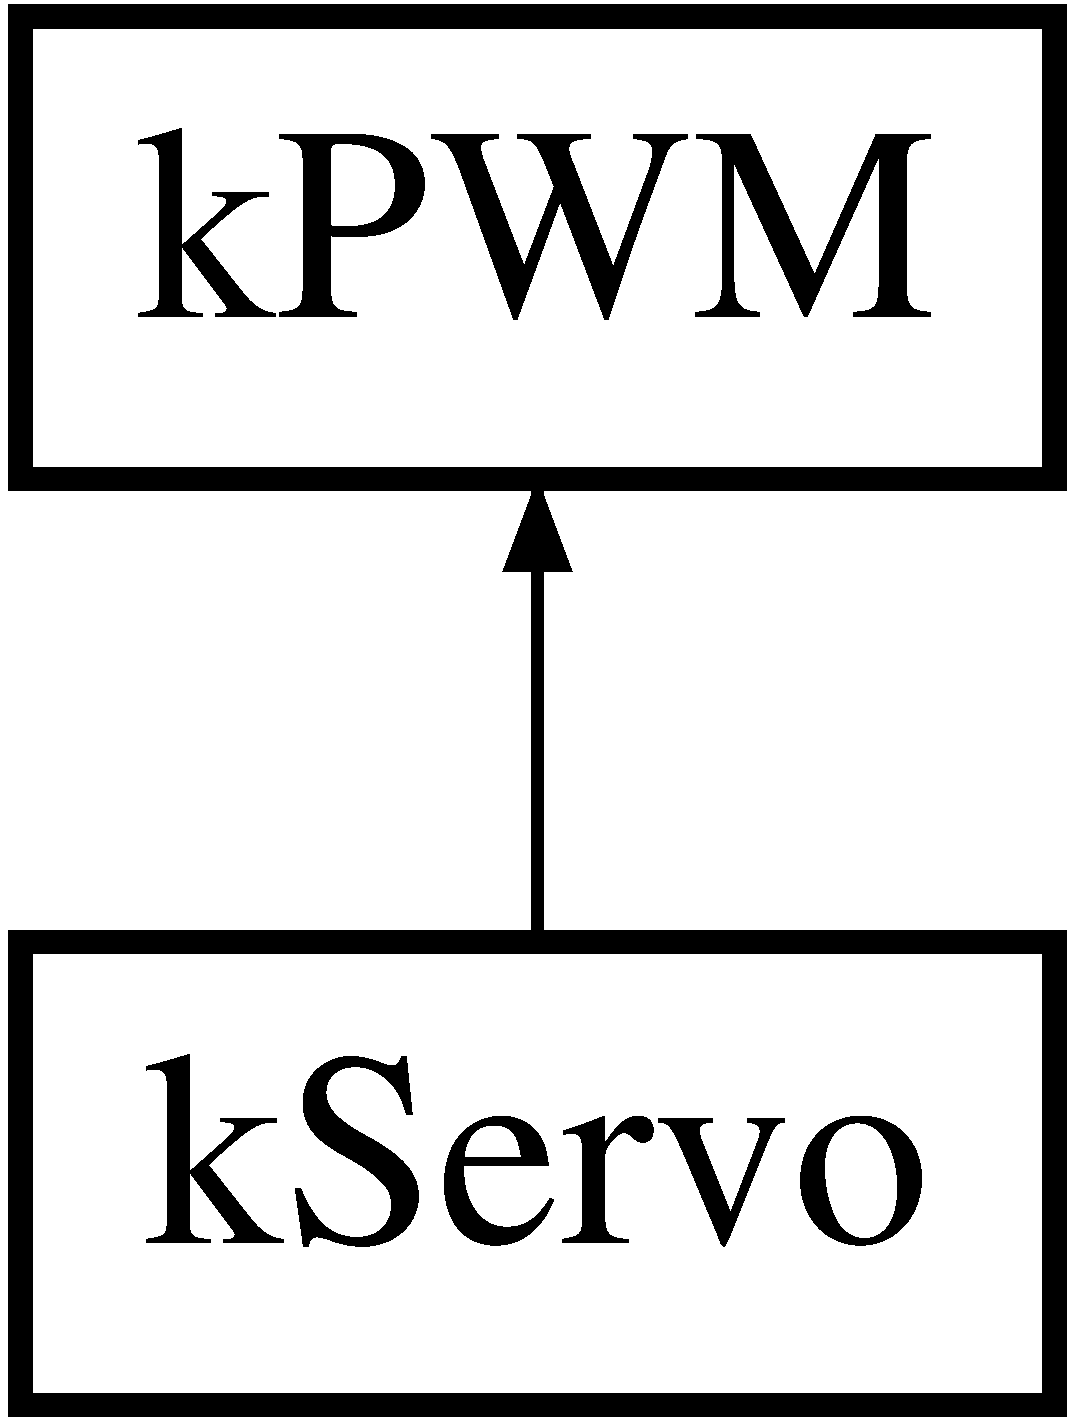
\includegraphics[height=2.000000cm]{classkServo}
\end{center}
\end{figure}
\subsection*{Public Member Functions}
\begin{DoxyCompactItemize}
\item 
void {\bfseries start} (float initial\+\_\+value=0.\+0)\hypertarget{classkServo_a57401b58c34287b31db5ed30889e9f47}{}\label{classkServo_a57401b58c34287b31db5ed30889e9f47}

\item 
void {\bfseries operator=} (float value)\hypertarget{classkServo_a9aa52b5e04059063f696618c53233676}{}\label{classkServo_a9aa52b5e04059063f696618c53233676}

\end{DoxyCompactItemize}
\subsection*{Additional Inherited Members}


The documentation for this class was generated from the following files\+:\begin{DoxyCompactItemize}
\item 
k\+Servo.\+h\item 
k\+Servo.\+cpp\end{DoxyCompactItemize}

\hypertarget{classkSPI}{}\section{k\+S\+PI Class Reference}
\label{classkSPI}\index{k\+S\+PI@{k\+S\+PI}}
\subsection*{Public Types}
\begin{DoxyCompactItemize}
\item 
enum {\bfseries k\+S\+P\+I\+Mode} \{ {\bfseries Master}, 
{\bfseries Slave}
 \}\hypertarget{classkSPI_a3f875283cf2422b8b7213590599d2a54}{}\label{classkSPI_a3f875283cf2422b8b7213590599d2a54}

\item 
enum {\bfseries k\+S\+P\+I\+\_\+\+N\+S\+S\+\_\+\+Control} \{ {\bfseries N\+S\+S\+\_\+\+Hard\+\_\+\+Control}, 
{\bfseries N\+S\+S\+\_\+\+Soft\+\_\+\+Control}
 \}\hypertarget{classkSPI_af2847321cd94eccce2634b8edb193471}{}\label{classkSPI_af2847321cd94eccce2634b8edb193471}

\item 
enum {\bfseries k\+S\+P\+I\+\_\+\+Transfer\+Bit\+First} \{ {\bfseries M\+S\+B\+\_\+\+First}, 
{\bfseries L\+S\+B\+\_\+\+First}
 \}\hypertarget{classkSPI_ae4b5e7a7b02c6db8906b7a1ad4f56ad8}{}\label{classkSPI_ae4b5e7a7b02c6db8906b7a1ad4f56ad8}

\item 
enum {\bfseries k\+S\+P\+I\+\_\+\+Baud} \{ \\*
{\bfseries Baud\+Div\+\_\+2}, 
{\bfseries Baud\+Div\+\_\+4}, 
{\bfseries Baud\+Div\+\_\+8}, 
{\bfseries Baud\+Div\+\_\+16}, 
\\*
{\bfseries Baud\+Div\+\_\+32}, 
{\bfseries Baud\+Div\+\_\+64}, 
{\bfseries Baud\+Div\+\_\+128}, 
{\bfseries Baud\+Div\+\_\+256}
 \}\hypertarget{classkSPI_a015f6611cec7b59fbf631625d1cac0b2}{}\label{classkSPI_a015f6611cec7b59fbf631625d1cac0b2}

\item 
enum {\bfseries k\+S\+P\+I\+\_\+\+C\+P\+OL} \{ {\bfseries S\+C\+K\+\_\+\+Idle\+Low}, 
{\bfseries S\+C\+K\+\_\+\+Idle\+High}
 \}\hypertarget{classkSPI_ac532bae095b82181c9485a464d8209e1}{}\label{classkSPI_ac532bae095b82181c9485a464d8209e1}

\item 
enum {\bfseries k\+S\+P\+I\+\_\+\+C\+P\+HA} \{ {\bfseries Data\+Capture\+\_\+1\+Edge}, 
{\bfseries Data\+Capture\+\_\+2\+Edge}
 \}\hypertarget{classkSPI_aafaa3b8faa71a2d707da7bde204999d3}{}\label{classkSPI_aafaa3b8faa71a2d707da7bde204999d3}

\item 
enum {\bfseries k\+S\+P\+I\+\_\+power} \{ {\bfseries off}, 
{\bfseries on}
 \}\hypertarget{classkSPI_a37fdc25c9c10f284479c8b47198068fe}{}\label{classkSPI_a37fdc25c9c10f284479c8b47198068fe}

\end{DoxyCompactItemize}
\subsection*{Static Public Attributes}
\begin{DoxyCompactItemize}
\item 
static const \hyperlink{structkSPI1}{k\+S\+P\+I1} $\ast$ {\bfseries S\+P\+I\+\_\+1} = (\hyperlink{structkSPI1}{k\+S\+P\+I1} $\ast$)S\+R\+A\+M1\+\_\+\+B\+A\+SE\hypertarget{classkSPI_a0aa7c24357362d2ba703068b4259cfd0}{}\label{classkSPI_a0aa7c24357362d2ba703068b4259cfd0}

\end{DoxyCompactItemize}


The documentation for this class was generated from the following files\+:\begin{DoxyCompactItemize}
\item 
k\+S\+P\+I\+Device.\+h\item 
k\+S\+P\+I\+Device.\+cpp\end{DoxyCompactItemize}

\hypertarget{structkSPI1}{}\section{k\+S\+P\+I1 Struct Reference}
\label{structkSPI1}\index{k\+S\+P\+I1@{k\+S\+P\+I1}}
\subsection*{Public Attributes}
\begin{DoxyCompactItemize}
\item 
\hyperlink{structkSPI1__MISO__Pin}{k\+S\+P\+I1\+\_\+\+M\+I\+S\+O\+\_\+\+Pin} {\bfseries M\+I\+SO}\hypertarget{structkSPI1_ac63e07e554c99cd319ed780a567ec77f}{}\label{structkSPI1_ac63e07e554c99cd319ed780a567ec77f}

\item 
\hyperlink{structkSPI1__MOSI__Pin}{k\+S\+P\+I1\+\_\+\+M\+O\+S\+I\+\_\+\+Pin} {\bfseries M\+O\+SI}\hypertarget{structkSPI1_a54cbe73c217faf27131a6d37fd159dae}{}\label{structkSPI1_a54cbe73c217faf27131a6d37fd159dae}

\item 
\hyperlink{structkSPI1__NSS__Pin}{k\+S\+P\+I1\+\_\+\+N\+S\+S\+\_\+\+Pin} {\bfseries N\+SS}\hypertarget{structkSPI1_a8fa4ced92a9ced00a041e7e5d25e728a}{}\label{structkSPI1_a8fa4ced92a9ced00a041e7e5d25e728a}

\item 
\hyperlink{structkSPI1__SCK__Pin}{k\+S\+P\+I1\+\_\+\+S\+C\+K\+\_\+\+Pin} {\bfseries S\+CK}\hypertarget{structkSPI1_a6602ea3bcd980860bdc9ba0d93dc216c}{}\label{structkSPI1_a6602ea3bcd980860bdc9ba0d93dc216c}

\end{DoxyCompactItemize}


The documentation for this struct was generated from the following file\+:\begin{DoxyCompactItemize}
\item 
k\+S\+P\+I\+Device.\+h\end{DoxyCompactItemize}

\hypertarget{structkSPI1__MISO__Pin}{}\section{k\+S\+P\+I1\+\_\+\+M\+I\+S\+O\+\_\+\+Pin Struct Reference}
\label{structkSPI1__MISO__Pin}\index{k\+S\+P\+I1\+\_\+\+M\+I\+S\+O\+\_\+\+Pin@{k\+S\+P\+I1\+\_\+\+M\+I\+S\+O\+\_\+\+Pin}}
\subsection*{Public Attributes}
\begin{DoxyCompactItemize}
\item 
\hyperlink{structkSPI1pin}{k\+S\+P\+I1pin} {\bfseries P\+O\+R\+T\+A6}\hypertarget{structkSPI1__MISO__Pin_a1a63604619ef35ba18b20008d1764161}{}\label{structkSPI1__MISO__Pin_a1a63604619ef35ba18b20008d1764161}

\item 
\hyperlink{structkSPI1pin}{k\+S\+P\+I1pin} {\bfseries P\+O\+R\+T\+B4}\hypertarget{structkSPI1__MISO__Pin_a686d8c72a421ccadb96418c3e616a013}{}\label{structkSPI1__MISO__Pin_a686d8c72a421ccadb96418c3e616a013}

\end{DoxyCompactItemize}


The documentation for this struct was generated from the following file\+:\begin{DoxyCompactItemize}
\item 
k\+S\+P\+I\+Device.\+h\end{DoxyCompactItemize}

\hypertarget{structkSPI1__MOSI__Pin}{}\section{k\+S\+P\+I1\+\_\+\+M\+O\+S\+I\+\_\+\+Pin Struct Reference}
\label{structkSPI1__MOSI__Pin}\index{k\+S\+P\+I1\+\_\+\+M\+O\+S\+I\+\_\+\+Pin@{k\+S\+P\+I1\+\_\+\+M\+O\+S\+I\+\_\+\+Pin}}
\subsection*{Public Attributes}
\begin{DoxyCompactItemize}
\item 
\hyperlink{structkSPI1pin}{k\+S\+P\+I1pin} {\bfseries P\+O\+R\+T\+A7}\hypertarget{structkSPI1__MOSI__Pin_a54502731f7d03db868899508b35797be}{}\label{structkSPI1__MOSI__Pin_a54502731f7d03db868899508b35797be}

\item 
\hyperlink{structkSPI1pin}{k\+S\+P\+I1pin} {\bfseries P\+O\+R\+T\+B5}\hypertarget{structkSPI1__MOSI__Pin_a4c4028cd0ad97461fd4cd356bd0011ba}{}\label{structkSPI1__MOSI__Pin_a4c4028cd0ad97461fd4cd356bd0011ba}

\end{DoxyCompactItemize}


The documentation for this struct was generated from the following file\+:\begin{DoxyCompactItemize}
\item 
k\+S\+P\+I\+Device.\+h\end{DoxyCompactItemize}

\hypertarget{structkSPI1__NSS__Pin}{}\section{k\+S\+P\+I1\+\_\+\+N\+S\+S\+\_\+\+Pin Struct Reference}
\label{structkSPI1__NSS__Pin}\index{k\+S\+P\+I1\+\_\+\+N\+S\+S\+\_\+\+Pin@{k\+S\+P\+I1\+\_\+\+N\+S\+S\+\_\+\+Pin}}
\subsection*{Public Attributes}
\begin{DoxyCompactItemize}
\item 
\hyperlink{structkSPI1pin}{k\+S\+P\+I1pin} {\bfseries P\+O\+R\+T\+A4}\hypertarget{structkSPI1__NSS__Pin_a270ede5256c319cba8bb927534ee0cab}{}\label{structkSPI1__NSS__Pin_a270ede5256c319cba8bb927534ee0cab}

\item 
\hyperlink{structkSPI1pin}{k\+S\+P\+I1pin} {\bfseries P\+O\+R\+T\+A15}\hypertarget{structkSPI1__NSS__Pin_ad69180293da9e411bd88eb9a270d191a}{}\label{structkSPI1__NSS__Pin_ad69180293da9e411bd88eb9a270d191a}

\end{DoxyCompactItemize}


The documentation for this struct was generated from the following file\+:\begin{DoxyCompactItemize}
\item 
k\+S\+P\+I\+Device.\+h\end{DoxyCompactItemize}

\hypertarget{structkSPI1__SCK__Pin}{}\section{k\+S\+P\+I1\+\_\+\+S\+C\+K\+\_\+\+Pin Struct Reference}
\label{structkSPI1__SCK__Pin}\index{k\+S\+P\+I1\+\_\+\+S\+C\+K\+\_\+\+Pin@{k\+S\+P\+I1\+\_\+\+S\+C\+K\+\_\+\+Pin}}
\subsection*{Public Attributes}
\begin{DoxyCompactItemize}
\item 
\hyperlink{structkSPI1pin}{k\+S\+P\+I1pin} {\bfseries P\+O\+R\+T\+A5}\hypertarget{structkSPI1__SCK__Pin_a04f1a5d6e5a2339851fc1259b4fcd90e}{}\label{structkSPI1__SCK__Pin_a04f1a5d6e5a2339851fc1259b4fcd90e}

\item 
\hyperlink{structkSPI1pin}{k\+S\+P\+I1pin} {\bfseries P\+O\+R\+T\+B3}\hypertarget{structkSPI1__SCK__Pin_a662a38a8964e8dad2ee4fc6d63034a7e}{}\label{structkSPI1__SCK__Pin_a662a38a8964e8dad2ee4fc6d63034a7e}

\end{DoxyCompactItemize}


The documentation for this struct was generated from the following file\+:\begin{DoxyCompactItemize}
\item 
k\+S\+P\+I\+Device.\+h\end{DoxyCompactItemize}

\hypertarget{structkSPI1pin}{}\section{k\+S\+P\+I1pin Struct Reference}
\label{structkSPI1pin}\index{k\+S\+P\+I1pin@{k\+S\+P\+I1pin}}
\subsection*{Public Attributes}
\begin{DoxyCompactItemize}
\item 
unsigned char {\bfseries k\+S\+P\+Ipin}\hypertarget{structkSPI1pin_ab931827287d8d6bac69c5557e9790ff3}{}\label{structkSPI1pin_ab931827287d8d6bac69c5557e9790ff3}

\end{DoxyCompactItemize}


The documentation for this struct was generated from the following file\+:\begin{DoxyCompactItemize}
\item 
k\+S\+P\+I\+Device.\+h\end{DoxyCompactItemize}

\hypertarget{classkSPIDevice}{}\section{k\+S\+P\+I\+Device Class Reference}
\label{classkSPIDevice}\index{k\+S\+P\+I\+Device@{k\+S\+P\+I\+Device}}
Inheritance diagram for k\+S\+P\+I\+Device\+:\begin{figure}[H]
\begin{center}
\leavevmode
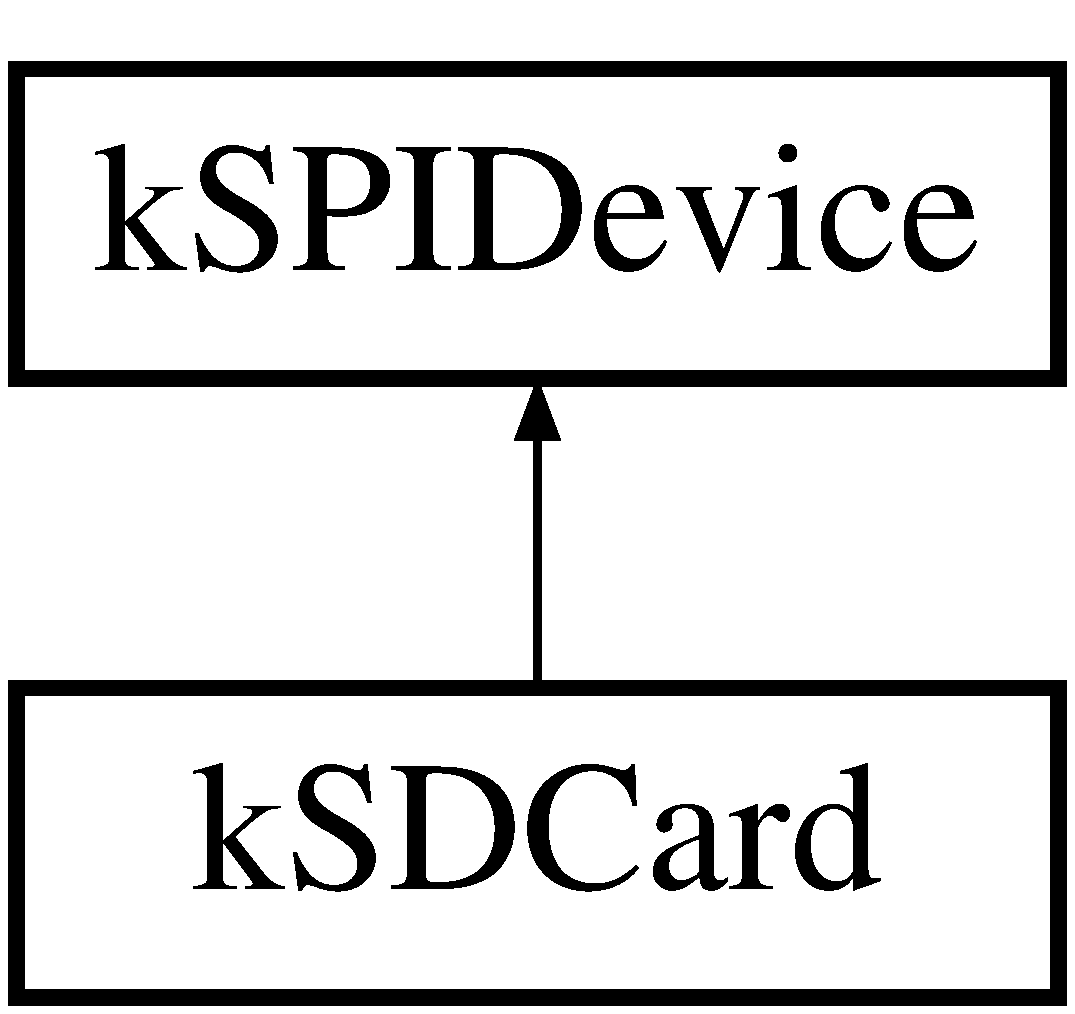
\includegraphics[height=2.000000cm]{classkSPIDevice}
\end{center}
\end{figure}
\subsection*{Public Member Functions}
\begin{DoxyCompactItemize}
\item 
void {\bfseries write} (unsigned short int Bytes\+To\+Write, unsigned char $\ast$Data\+Buffer)\hypertarget{classkSPIDevice_afed454ddc1a7563ac3e2b2c81e2f30cf}{}\label{classkSPIDevice_afed454ddc1a7563ac3e2b2c81e2f30cf}

\item 
void {\bfseries write} (unsigned char Byte)\hypertarget{classkSPIDevice_a5d91795858db810e3cb6240e7d3ab6c2}{}\label{classkSPIDevice_a5d91795858db810e3cb6240e7d3ab6c2}

\item 
void {\bfseries read} (unsigned short int Bytes\+To\+Read, unsigned char $\ast$Read\+Data\+Buffer)\hypertarget{classkSPIDevice_a6198701733aa49a62197e8e352b91612}{}\label{classkSPIDevice_a6198701733aa49a62197e8e352b91612}

\item 
unsigned char {\bfseries read} (void)\hypertarget{classkSPIDevice_adae1ee49e21ed5e671488855b9156357}{}\label{classkSPIDevice_adae1ee49e21ed5e671488855b9156357}

\item 
void {\bfseries select} (void)\hypertarget{classkSPIDevice_a5fd0c88a3ea09d019cb2f5f187b05a6d}{}\label{classkSPIDevice_a5fd0c88a3ea09d019cb2f5f187b05a6d}

\item 
void {\bfseries deselect} (void)\hypertarget{classkSPIDevice_a50490cb2c1563b5c7f2ec2c52d30b2fd}{}\label{classkSPIDevice_a50490cb2c1563b5c7f2ec2c52d30b2fd}

\end{DoxyCompactItemize}
\subsection*{Public Attributes}
\begin{DoxyCompactItemize}
\item 
\hyperlink{classkSPIDeviceHardware}{k\+S\+P\+I\+Device\+Hardware} {\bfseries hardware}\hypertarget{classkSPIDevice_a9713a103f247eef36a68e26318c93bef}{}\label{classkSPIDevice_a9713a103f247eef36a68e26318c93bef}

\end{DoxyCompactItemize}


The documentation for this class was generated from the following files\+:\begin{DoxyCompactItemize}
\item 
k\+S\+P\+I\+Device.\+h\item 
k\+S\+P\+I\+Device.\+cpp\end{DoxyCompactItemize}

\hypertarget{classkSPIDeviceHardware}{}\section{k\+S\+P\+I\+Device\+Hardware Class Reference}
\label{classkSPIDeviceHardware}\index{k\+S\+P\+I\+Device\+Hardware@{k\+S\+P\+I\+Device\+Hardware}}
\subsection*{Public Member Functions}
\begin{DoxyCompactItemize}
\item 
\hyperlink{classkSPIDeviceHardware}{k\+S\+P\+I\+Device\+Hardware} \& {\bfseries operator=} (const \hyperlink{structkSPI1pin}{k\+S\+P\+I1pin} \&spi\+Hard)\hypertarget{classkSPIDeviceHardware_a169e7e9d2a6d4ae7a220c9026959cc9c}{}\label{classkSPIDeviceHardware_a169e7e9d2a6d4ae7a220c9026959cc9c}

\item 
\hyperlink{classkSPIDeviceHardware}{k\+S\+P\+I\+Device\+Hardware} \& {\bfseries operator=} (const k\+S\+P\+I\+::k\+S\+P\+I\+Mode mode)\hypertarget{classkSPIDeviceHardware_a5ba117f50e6dae7f5d91f0d2624d588c}{}\label{classkSPIDeviceHardware_a5ba117f50e6dae7f5d91f0d2624d588c}

\item 
\hyperlink{classkSPIDeviceHardware}{k\+S\+P\+I\+Device\+Hardware} \& {\bfseries operator=} (const k\+S\+P\+I\+::k\+S\+P\+I\+\_\+\+Baud baud)\hypertarget{classkSPIDeviceHardware_a3167c104f7eb427144de555ffe700d90}{}\label{classkSPIDeviceHardware_a3167c104f7eb427144de555ffe700d90}

\item 
\hyperlink{classkSPIDeviceHardware}{k\+S\+P\+I\+Device\+Hardware} \& {\bfseries operator=} (const k\+S\+P\+I\+::k\+S\+P\+I\+\_\+\+C\+P\+HA cpha)\hypertarget{classkSPIDeviceHardware_a0c39789100f567dd509cba4fa7573363}{}\label{classkSPIDeviceHardware_a0c39789100f567dd509cba4fa7573363}

\item 
\hyperlink{classkSPIDeviceHardware}{k\+S\+P\+I\+Device\+Hardware} \& {\bfseries operator=} (const k\+S\+P\+I\+::k\+S\+P\+I\+\_\+\+C\+P\+OL cpol)\hypertarget{classkSPIDeviceHardware_a4cd32775d02a9677089744187cb00e63}{}\label{classkSPIDeviceHardware_a4cd32775d02a9677089744187cb00e63}

\item 
\hyperlink{classkSPIDeviceHardware}{k\+S\+P\+I\+Device\+Hardware} \& {\bfseries operator=} (const k\+S\+P\+I\+::k\+S\+P\+I\+\_\+\+N\+S\+S\+\_\+\+Control nss\+\_\+control)\hypertarget{classkSPIDeviceHardware_a252c8ca08d3472103ee9cd2d74b48894}{}\label{classkSPIDeviceHardware_a252c8ca08d3472103ee9cd2d74b48894}

\item 
\hyperlink{classkSPIDeviceHardware}{k\+S\+P\+I\+Device\+Hardware} \& {\bfseries operator=} (const k\+S\+P\+I\+::k\+S\+P\+I\+\_\+\+Transfer\+Bit\+First endian)\hypertarget{classkSPIDeviceHardware_a522099238f3bad48a79f93b020ac24c5}{}\label{classkSPIDeviceHardware_a522099238f3bad48a79f93b020ac24c5}

\item 
\hyperlink{classkSPIDeviceHardware}{k\+S\+P\+I\+Device\+Hardware} \& {\bfseries operator=} (const k\+S\+P\+I\+::k\+S\+P\+I\+\_\+power pow)\hypertarget{classkSPIDeviceHardware_ae426a4bfdebc93c6bc881389b877361d}{}\label{classkSPIDeviceHardware_ae426a4bfdebc93c6bc881389b877361d}

\item 
void {\bfseries setup\+M\+I\+S\+O\+Pin} (void)\hypertarget{classkSPIDeviceHardware_ad7d69f31bbdde466f70a36a430725bf5}{}\label{classkSPIDeviceHardware_ad7d69f31bbdde466f70a36a430725bf5}

\item 
void {\bfseries setup\+M\+O\+S\+I\+Pin} (void)\hypertarget{classkSPIDeviceHardware_a1ecbe2c47374eae569823e42aa935626}{}\label{classkSPIDeviceHardware_a1ecbe2c47374eae569823e42aa935626}

\item 
void {\bfseries setup\+N\+S\+S\+Pin} (void)\hypertarget{classkSPIDeviceHardware_a3a4ba8b61620a400cfc0264eb102d26f}{}\label{classkSPIDeviceHardware_a3a4ba8b61620a400cfc0264eb102d26f}

\item 
void {\bfseries setup\+S\+C\+K\+Pin} (void)\hypertarget{classkSPIDeviceHardware_a37830215a2358c18770d3900db3db1c9}{}\label{classkSPIDeviceHardware_a37830215a2358c18770d3900db3db1c9}

\end{DoxyCompactItemize}
\subsection*{Public Attributes}
\begin{DoxyCompactItemize}
\item 
unsigned char {\bfseries N\+S\+S\+\_\+idle\+State}\hypertarget{classkSPIDeviceHardware_a184c85b6972b61c1ebf1d687b8f7bd82}{}\label{classkSPIDeviceHardware_a184c85b6972b61c1ebf1d687b8f7bd82}

\item 
S\+P\+I\+\_\+\+Type\+Def $\ast$ {\bfseries spi}\hypertarget{classkSPIDeviceHardware_a60947ab698497000006280ef5ecb092a}{}\label{classkSPIDeviceHardware_a60947ab698497000006280ef5ecb092a}

\item 
G\+P\+I\+O\+\_\+\+Type\+Def $\ast$ {\bfseries miso\+G\+P\+IO}\hypertarget{classkSPIDeviceHardware_a25b81d06ecaafaf6fae5b68936a32377}{}\label{classkSPIDeviceHardware_a25b81d06ecaafaf6fae5b68936a32377}

\item 
G\+P\+I\+O\+\_\+\+Type\+Def $\ast$ {\bfseries mosi\+G\+P\+IO}\hypertarget{classkSPIDeviceHardware_af03dcd681ecac4e925bf538f9d7327d2}{}\label{classkSPIDeviceHardware_af03dcd681ecac4e925bf538f9d7327d2}

\item 
G\+P\+I\+O\+\_\+\+Type\+Def $\ast$ {\bfseries nss\+G\+P\+IO}\hypertarget{classkSPIDeviceHardware_a1a3747b1876322b63cfa1d8ec95b1a99}{}\label{classkSPIDeviceHardware_a1a3747b1876322b63cfa1d8ec95b1a99}

\item 
G\+P\+I\+O\+\_\+\+Type\+Def $\ast$ {\bfseries sck\+G\+P\+IO}\hypertarget{classkSPIDeviceHardware_a53942221b7462728e5c1581d9fcd4f3b}{}\label{classkSPIDeviceHardware_a53942221b7462728e5c1581d9fcd4f3b}

\item 
unsigned char {\bfseries miso\+Pin}\hypertarget{classkSPIDeviceHardware_a9a0da5c69aa11f1305b01478ae60160f}{}\label{classkSPIDeviceHardware_a9a0da5c69aa11f1305b01478ae60160f}

\item 
unsigned char {\bfseries mosi\+Pin}\hypertarget{classkSPIDeviceHardware_ac57e11d1574088108499a4d76474f58f}{}\label{classkSPIDeviceHardware_ac57e11d1574088108499a4d76474f58f}

\item 
unsigned char {\bfseries nss\+Pin}\hypertarget{classkSPIDeviceHardware_a3793deec821e7b106cb4a6ff58dcfabf}{}\label{classkSPIDeviceHardware_a3793deec821e7b106cb4a6ff58dcfabf}

\item 
unsigned char {\bfseries sck\+Pin}\hypertarget{classkSPIDeviceHardware_a7b2df59124faa6debdaf473748ee0b92}{}\label{classkSPIDeviceHardware_a7b2df59124faa6debdaf473748ee0b92}

\end{DoxyCompactItemize}
\subsection*{Friends}
\begin{DoxyCompactItemize}
\item 
\hyperlink{classkSPIDeviceHardware}{k\+S\+P\+I\+Device\+Hardware} \& {\bfseries operator,} (\hyperlink{classkSPIDeviceHardware}{k\+S\+P\+I\+Device\+Hardware} \&spi\+Dev, const \hyperlink{structkSPI1pin}{k\+S\+P\+I1pin} \&spi\+Hard)\hypertarget{classkSPIDeviceHardware_a233dc15697785ac12db215087a19977b}{}\label{classkSPIDeviceHardware_a233dc15697785ac12db215087a19977b}

\item 
\hyperlink{classkSPIDeviceHardware}{k\+S\+P\+I\+Device\+Hardware} \& {\bfseries operator,} (\hyperlink{classkSPIDeviceHardware}{k\+S\+P\+I\+Device\+Hardware} \&spi\+Dev, const k\+S\+P\+I\+::k\+S\+P\+I\+Mode mode)\hypertarget{classkSPIDeviceHardware_a38f361c44f1d601d4070393dc713220f}{}\label{classkSPIDeviceHardware_a38f361c44f1d601d4070393dc713220f}

\item 
\hyperlink{classkSPIDeviceHardware}{k\+S\+P\+I\+Device\+Hardware} \& {\bfseries operator,} (\hyperlink{classkSPIDeviceHardware}{k\+S\+P\+I\+Device\+Hardware} \&spi\+Dev, const k\+S\+P\+I\+::k\+S\+P\+I\+\_\+\+Baud baud)\hypertarget{classkSPIDeviceHardware_ac79b4c18515b69dffa81066e69b23791}{}\label{classkSPIDeviceHardware_ac79b4c18515b69dffa81066e69b23791}

\item 
\hyperlink{classkSPIDeviceHardware}{k\+S\+P\+I\+Device\+Hardware} \& {\bfseries operator,} (\hyperlink{classkSPIDeviceHardware}{k\+S\+P\+I\+Device\+Hardware} \&spi\+Dev, const k\+S\+P\+I\+::k\+S\+P\+I\+\_\+\+C\+P\+HA cpha)\hypertarget{classkSPIDeviceHardware_acf00881fad01697aa7ff8c058618969f}{}\label{classkSPIDeviceHardware_acf00881fad01697aa7ff8c058618969f}

\item 
\hyperlink{classkSPIDeviceHardware}{k\+S\+P\+I\+Device\+Hardware} \& {\bfseries operator,} (\hyperlink{classkSPIDeviceHardware}{k\+S\+P\+I\+Device\+Hardware} \&spi\+Dev, const k\+S\+P\+I\+::k\+S\+P\+I\+\_\+\+C\+P\+OL cpol)\hypertarget{classkSPIDeviceHardware_acf990179b76570518d59ce6baa7be6cf}{}\label{classkSPIDeviceHardware_acf990179b76570518d59ce6baa7be6cf}

\item 
\hyperlink{classkSPIDeviceHardware}{k\+S\+P\+I\+Device\+Hardware} \& {\bfseries operator,} (\hyperlink{classkSPIDeviceHardware}{k\+S\+P\+I\+Device\+Hardware} \&spi\+Dev, const k\+S\+P\+I\+::k\+S\+P\+I\+\_\+\+N\+S\+S\+\_\+\+Control nss\+\_\+control)\hypertarget{classkSPIDeviceHardware_aecea7355baf6a0481936de37539431f0}{}\label{classkSPIDeviceHardware_aecea7355baf6a0481936de37539431f0}

\item 
\hyperlink{classkSPIDeviceHardware}{k\+S\+P\+I\+Device\+Hardware} \& {\bfseries operator,} (\hyperlink{classkSPIDeviceHardware}{k\+S\+P\+I\+Device\+Hardware} \&spi\+Dev, const k\+S\+P\+I\+::k\+S\+P\+I\+\_\+\+Transfer\+Bit\+First endian)\hypertarget{classkSPIDeviceHardware_addfb62b4b46014f54cfb049134c36117}{}\label{classkSPIDeviceHardware_addfb62b4b46014f54cfb049134c36117}

\item 
\hyperlink{classkSPIDeviceHardware}{k\+S\+P\+I\+Device\+Hardware} \& {\bfseries operator,} (\hyperlink{classkSPIDeviceHardware}{k\+S\+P\+I\+Device\+Hardware} \&spi\+Dev, const k\+S\+P\+I\+::k\+S\+P\+I\+\_\+power pow)\hypertarget{classkSPIDeviceHardware_a5962811e308e7fc7dca2fcb1e5da8c5c}{}\label{classkSPIDeviceHardware_a5962811e308e7fc7dca2fcb1e5da8c5c}

\end{DoxyCompactItemize}


The documentation for this class was generated from the following files\+:\begin{DoxyCompactItemize}
\item 
k\+S\+P\+I\+Device.\+h\item 
k\+S\+P\+I\+Device.\+cpp\end{DoxyCompactItemize}

\hypertarget{classkString}{}\section{k\+String Class Reference}
\label{classkString}\index{k\+String@{k\+String}}
\subsection*{Public Member Functions}
\begin{DoxyCompactItemize}
\item 
{\bfseries k\+String} (const \hyperlink{classkString}{k\+String} \&other)\hypertarget{classkString_a723ed0f36a930c34e1f377422dc6cb87}{}\label{classkString_a723ed0f36a930c34e1f377422dc6cb87}

\item 
{\bfseries k\+String} (const char $\ast$str)\hypertarget{classkString_a34ba9c86d2cbcdd64af7f85e02881514}{}\label{classkString_a34ba9c86d2cbcdd64af7f85e02881514}

\item 
unsigned short {\bfseries length} (void) const \hypertarget{classkString_afcf0a1db915e2de54622e203d45ef31c}{}\label{classkString_afcf0a1db915e2de54622e203d45ef31c}

\item 
bool {\bfseries is\+Empty} (void)\hypertarget{classkString_ac17f389b5b95b86e014d75e4e1f17d60}{}\label{classkString_ac17f389b5b95b86e014d75e4e1f17d60}

\item 
unsigned char $\ast$ {\bfseries c\+\_\+str} (void) const \hypertarget{classkString_ad2b0506e7c45c88a6f48713b7fd9dbe2}{}\label{classkString_ad2b0506e7c45c88a6f48713b7fd9dbe2}

\item 
\hyperlink{classkString}{k\+String} {\bfseries get\+Substring} (char delimiter, unsigned char returned\+\_\+part)\hypertarget{classkString_a57cd7485bb48d98f4bdc774473d3eeab}{}\label{classkString_a57cd7485bb48d98f4bdc774473d3eeab}

\item 
void {\bfseries operator=} (const char $\ast$str)\hypertarget{classkString_a01694244979403aa17c4d3e4bd43393d}{}\label{classkString_a01694244979403aa17c4d3e4bd43393d}

\item 
void {\bfseries operator=} (const \hyperlink{classkString}{k\+String} \&str)\hypertarget{classkString_a7e4e68f3b38f121fe5fc4a0b8bdb2649}{}\label{classkString_a7e4e68f3b38f121fe5fc4a0b8bdb2649}

\item 
void {\bfseries operator+=} (const char $\ast$str)\hypertarget{classkString_a28831f6691370791b951e79607e3cac4}{}\label{classkString_a28831f6691370791b951e79607e3cac4}

\item 
void {\bfseries operator+=} (const \hyperlink{classkString}{k\+String} \&str)\hypertarget{classkString_a4cbf038b684ad999859193bf817c9ced}{}\label{classkString_a4cbf038b684ad999859193bf817c9ced}

\item 
const \hyperlink{classkString}{k\+String} {\bfseries operator+} (const \hyperlink{classkString}{k\+String} \&str)\hypertarget{classkString_a0e1b752818605ce0341c1147c3715cad}{}\label{classkString_a0e1b752818605ce0341c1147c3715cad}

\item 
const \hyperlink{classkString}{k\+String} {\bfseries operator+} (const char $\ast$str)\hypertarget{classkString_aebf22a94f69ca121c3421fc7a1bcb8ce}{}\label{classkString_aebf22a94f69ca121c3421fc7a1bcb8ce}

\item 
int {\bfseries to\+Int} (void)\hypertarget{classkString_a449a427129336d7a8c512e455c612080}{}\label{classkString_a449a427129336d7a8c512e455c612080}

\item 
float {\bfseries to\+Float} (void)\hypertarget{classkString_affa35f1556633e044cd19d8745ff8a82}{}\label{classkString_affa35f1556633e044cd19d8745ff8a82}

\end{DoxyCompactItemize}
\subsection*{Static Public Member Functions}
\begin{DoxyCompactItemize}
\item 
static \hyperlink{classkString}{k\+String} {\bfseries number} (int number)\hypertarget{classkString_ab4e1378470483b703ef29b700032860d}{}\label{classkString_ab4e1378470483b703ef29b700032860d}

\item 
static const \hyperlink{classkString}{k\+String} {\bfseries number} (float number, unsigned char precision=2)\hypertarget{classkString_a34bef8ee73be49f5d2151b3e0a51eab4}{}\label{classkString_a34bef8ee73be49f5d2151b3e0a51eab4}

\end{DoxyCompactItemize}
\subsection*{Friends}
\begin{DoxyCompactItemize}
\item 
const \hyperlink{classkString}{k\+String} {\bfseries operator+} (const char $\ast$str1, \hyperlink{classkString}{k\+String} \&str2)\hypertarget{classkString_a8f69277eb781488af04069997190b36f}{}\label{classkString_a8f69277eb781488af04069997190b36f}

\end{DoxyCompactItemize}


The documentation for this class was generated from the following files\+:\begin{DoxyCompactItemize}
\item 
k\+String.\+h\item 
k\+String.\+cpp\end{DoxyCompactItemize}

\chapter{File Documentation}
\hypertarget{kPort_8h}{}\section{k\+Port.\+h File Reference}
\label{kPort_8h}\index{k\+Port.\+h@{k\+Port.\+h}}


This file contains all the classes and functions prototypes for using General Purpose Input Output.  


{\ttfamily \#include \char`\"{}stm32f4xx.\+h\char`\"{}}\\*
{\ttfamily \#include \char`\"{}stm32f4xx\+\_\+gpio.\+h\char`\"{}}\\*
\subsection*{Classes}
\begin{DoxyCompactItemize}
\item 
class \hyperlink{classkPin}{k\+Pin}
\begin{DoxyCompactList}\small\item\em \hyperlink{classkPin}{k\+Pin} class is used as abstract layer to handle input/output pin functionality \end{DoxyCompactList}\item 
class \hyperlink{classkPort}{k\+Port}
\begin{DoxyCompactList}\small\item\em G\+P\+IO abstract layer. \end{DoxyCompactList}\end{DoxyCompactItemize}
\subsection*{Variables}
\begin{DoxyCompactItemize}
\item 
\hyperlink{classkPort}{k\+Port} {\bfseries P\+O\+R\+TA}\hypertarget{kPort_8h_af51b6a20797a84db03d3726f701a2834}{}\label{kPort_8h_af51b6a20797a84db03d3726f701a2834}

\item 
\hyperlink{classkPort}{k\+Port} {\bfseries P\+O\+R\+TB}\hypertarget{kPort_8h_a407e693b703f2db49dfd9b31520332b9}{}\label{kPort_8h_a407e693b703f2db49dfd9b31520332b9}

\item 
\hyperlink{classkPort}{k\+Port} {\bfseries P\+O\+R\+TC}\hypertarget{kPort_8h_ae2d160d553181b8b14f98a1908bb9b9f}{}\label{kPort_8h_ae2d160d553181b8b14f98a1908bb9b9f}

\item 
\hyperlink{classkPort}{k\+Port} {\bfseries P\+O\+R\+TD}\hypertarget{kPort_8h_add01d2c4b1abe2e6e1b66c9ba1b32e3c}{}\label{kPort_8h_add01d2c4b1abe2e6e1b66c9ba1b32e3c}

\item 
\hyperlink{classkPort}{k\+Port} {\bfseries P\+O\+R\+TE}\hypertarget{kPort_8h_a34f46f0f3434f14925ccedcf36e76ff1}{}\label{kPort_8h_a34f46f0f3434f14925ccedcf36e76ff1}

\item 
\hyperlink{classkPort}{k\+Port} {\bfseries P\+O\+R\+TF}\hypertarget{kPort_8h_a4c6a74db4691c2bce2386d9f827f4136}{}\label{kPort_8h_a4c6a74db4691c2bce2386d9f827f4136}

\item 
\hyperlink{classkPort}{k\+Port} {\bfseries P\+O\+R\+TG}\hypertarget{kPort_8h_a0e5b3a7e1b0c7a8fe9e166b3e59ec31b}{}\label{kPort_8h_a0e5b3a7e1b0c7a8fe9e166b3e59ec31b}

\item 
\hyperlink{classkPort}{k\+Port} {\bfseries P\+O\+R\+TH}\hypertarget{kPort_8h_a171271c0d8ed25f87b9c884fd497fed0}{}\label{kPort_8h_a171271c0d8ed25f87b9c884fd497fed0}

\item 
\hyperlink{classkPort}{k\+Port} {\bfseries P\+O\+R\+TI}\hypertarget{kPort_8h_a0cd0225e6d985660a95d894e1a7eb2b7}{}\label{kPort_8h_a0cd0225e6d985660a95d894e1a7eb2b7}

\end{DoxyCompactItemize}


\subsection{Detailed Description}
This file contains all the classes and functions prototypes for using General Purpose Input Output. 

\begin{DoxyAuthor}{Author}
Paweł Zalewski 
\end{DoxyAuthor}
\begin{DoxyVersion}{Version}
V1.\+0.\+0 
\end{DoxyVersion}
\begin{DoxyDate}{Date}
29-\/\+October-\/2015 
\end{DoxyDate}

\chapter{Example Documentation}
\hypertarget{kPort_example_LED_8cpp-example}{}\section{k\+Port\+\_\+example\+\_\+\+L\+E\+D.\+cpp}
This example shows how to use \hyperlink{classkPin}{k\+Pin} class to control L\+ED diode


\begin{DoxyCodeInclude}
\textcolor{preprocessor}{#include "kSystem.h"}
\textcolor{preprocessor}{#include "\hyperlink{kPort_8h}{kPort.h}"}

\textcolor{keywordtype}{void} main(\textcolor{keywordtype}{void})
\{
    PORTA = kPort::on;      \textcolor{comment}{//Power on PORTA (by default is off)}
    \hyperlink{classkPin}{kPin} LED = PORTA[2];    \textcolor{comment}{//kPin declaration named LED attached to PORTA2}
    LED = \hyperlink{classkPin_a311ea70432d9c48754eacc8d8ce8a949acafa1712464c40b469cd18209d298967}{kPin::out};       \textcolor{comment}{//set LED pin as output (by default input mode selected)}

    \textcolor{keywordflow}{while}(1)
    \{
        \textcolor{comment}{// program main loop}
        
        kSystem.waitms(500);    \textcolor{comment}{// wait half a second}
        LED.\hyperlink{classkPin_af4c6220ae2ed038236d729f867940938}{toggle}();         \textcolor{comment}{// toggle LED state (blink LED)}
    \}


\}
\end{DoxyCodeInclude}
 
%--- End generated contents ---

% Index
\backmatter
\newpage
\phantomsection
\clearemptydoublepage
\addcontentsline{toc}{chapter}{Index}
\printindex

\end{document}
